\documentclass[
  babelLanguage=portuguese,
  final,
  %showtrims,
  %showwirebinding,
  webversion,
]{chantingbook}

\usepackage{local}

\title{Livro de Cânticos}
\subtitle{}

\begin{document}

\frontmatter

\webcover{%
% TODO: cover image in PT
%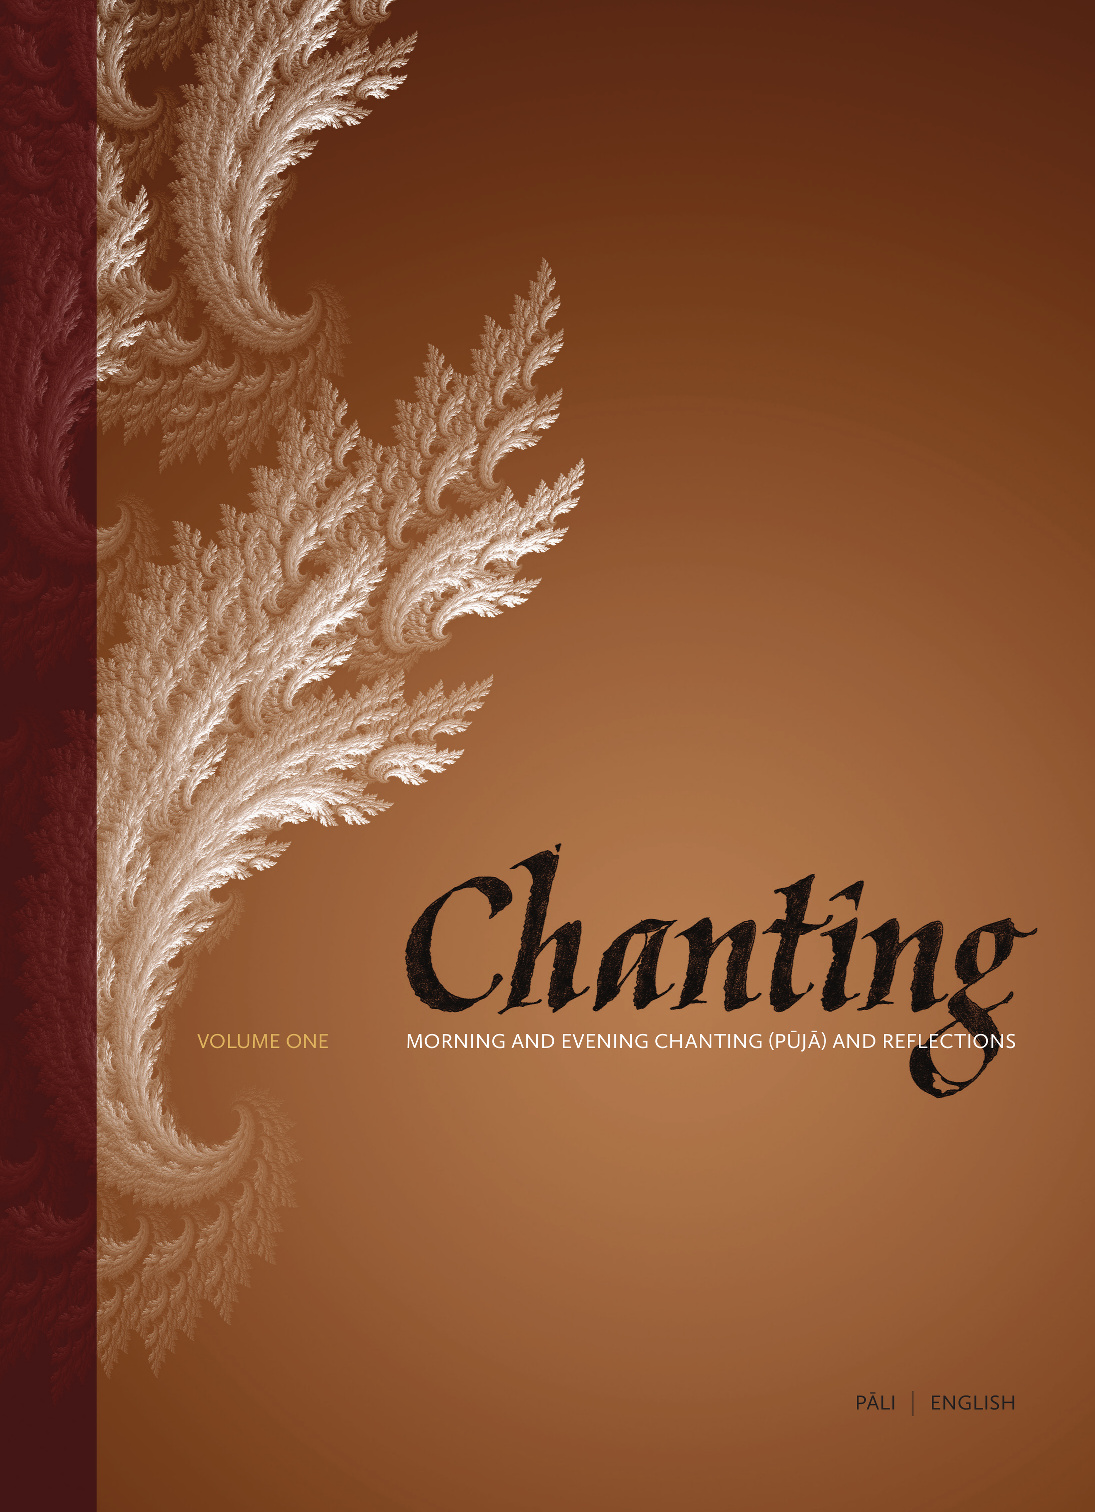
\includegraphics[height=\paperheight]{vol1-webcover.jpg}%

{\centering
\mbox{}
\vfill

\parttitlefont\color{chaptertitle}
%\addfontfeature{LetterSpace=2.0}

Livro de Cânticos

\vspace*{4\baselineskip}

\vfill

\mbox{}
}

}

% TODO: Copyright in PT

%\cleartoverso
%
\thispagestyle{empty}

\enlargethispage{\baselineskip}

{\centering\small
\setlength{\parskip}{15pt}

{\normalsize
\thetitle\\
\thesubtitle\\
Pāli and English}

Amaravati Publications\\
Amaravati Buddhist Monastery\\
St Margarets Lane\\
Great Gaddesden\\
Hemel Hempstead\\
Hertfordshire HP1 3BZ\\
UK\\
www.amaravati.org\\
(+44) (0)1442 842455

This book is offered for free distribution, please do not sell this book.\\
Also available for free download from:\\
www.forestsanghapublications.org

If you are interested in translating this text into another language,\\
please contact us at publications@amaravati.org

ISBN \theISBN

2015 \copyright\ Amaravati Buddhist Monastery

Project manager: Nicholas Halliday\\
Editor: Ajahn Amaro\\
Typesetting: Venerable Gambhīro\\
Cover lettering and design: Nicholas Halliday

\vfill

This work is licensed under a Creative Commons\\
Attribution-NonCommercial-NoDerivs 3.0 Unported Licence.\\
\href{http://creativecommons.org/licenses/by-nc-nd/3.0/}{http://creativecommons.org/licenses/by-nc-nd/3.0/}

See page \pageref{copyright-details} for more details on your rights and restrictions under this licence.

Produced with the \LaTeX\ typesetting system. Typeset in Gentium Incantation,\\
Alegreya Sans and Ubuntu fonts.

\theEditionInfo

\resizebox{15mm}{!}{\SanghaIcons\color{black!70} A}

}

% End of copyright.tex

%
%\cleartorecto
%\tableofcontents*
%
%\clearpage
%\chapterstyle{tocchapternoskip}
%\listfirstlines*

\mainmatter


% ===
\morningPartSettings

% TODO: morning chanting PT
\part{Cânticos Dias}

\morningChapterSettings

\chapter{Dedicação de Oferendas}

[Yo so] bha꜕gavā a꜕rahaṃ sammāsambuddho

\begin{english}
Ao Excelso, o Mestre, que totalmente alcançou a iluminação perfeita, 
\end{english}

Svākkhā꜓to yena bha꜕gava꜓tā dhammo

\begin{english}
Ao ensinamento, que Ele tão bem explicou,
\end{english}

Supaṭi꜕panno yassa bha꜕gava꜕to sāvaka꜕saṅgho

\begin{english}
E aos discípulos do Excelso, que tão bem praticaram,
\end{english}

Tam-ma꜓yaṃ bha꜕gavantaṃ sa꜕dhammaṃ sa꜕saṅghaṃ

\begin{english}
A estes – ao Buddha, ao Dhamma e ao Sangha ---
\end{english}

Imehi꜓ sakkārehi꜕ yathārahaṃ āropi꜕tehi a꜕bhi꜓pūja꜕yāma

\begin{english}
Apresentamos a devida homenagem com oferendas.
\end{english}

Sādhu꜓ no bhante bha꜕gavā su꜕cira-parinibbu꜕topi

\begin{english}
Para nós, é bom que tendo o Excelso se libertado,
\end{english}

Pacchi꜓mā-ja꜕na꜓tānu꜓kampa꜕-mānasā

\begin{english}
Ainda teve compaixão pelas gerações futuras.
\end{english}

Ime sakkāre dugga꜕ta꜕-paṇṇākāra꜓-bhūte pa꜕ṭiggaṇhātu

\begin{english}
Que estas simples oferendas sejam aceites
\end{english}

Amhā꜓kaṃ dīgha꜕rattaṃ hi꜕tāya su꜕khāya

\begin{english}
Pelo nosso duradouro benefício e pela felicidade que nos dá.
\end{english}

\clearpage

Arahaṃ sammāsambuddho bha꜕gavā

\begin{english}
Ao Mestre, O perfeitamente Iluminado e Excelso ---
\end{english}

Buddhaṃ bha꜕gavantaṃ a꜕bhi꜓vādemi

\begin{english}
  Ao Buddha, o Excelso, eu presto homenagem.
  \instr{Vénia}
\end{english}

[Svākkhā꜓to] bha꜕gava꜓tā dhammo

\begin{english}
 Ao ensinamento, tão plenamente explicado por Ele ---
\end{english}

Dhammaṃ namassāmi

\begin{english}
  Ao Dhamma, eu presto homenagem.
  \instr{Vénia}
\end{english}

[Supaṭi꜕panno] bha꜕gava꜕to sāvaka꜕saṅgho

\begin{english}
Aos discípulos do Excelso que tão bem praticaram ---
\end{english}

Sa꜓ṅghaṃ na꜕māmi

\begin{english}
  Ao Sangha, eu presto homenagem.
  \instr{Vénia}
\end{english}

\chapter{Homenagem Preliminar}

\begin{leader}
  [Ha꜓nda mayaṃ buddhassa꜕ bha꜕gavato pubbabhāga-namakā꜕raṃ karomase]
\end{leader}

\begin{english}
  [Prestemos agora homenagem preliminar ao Buddha.]
\end{english}

\vspace{\baselineskip}

Namo tassa bha꜕gava꜕to araha꜕to sa꜓mmāsa꜓mbuddha꜕ssa

\instr{Três vezes}

\begin{english}
  Homenagem ao Excelso, Nobre e Perfeitamente Iluminado.

  \instr{Três vezes}
\end{english}

\clearpage

\chapter{Homenagem ao Buddha}

\begin{leader}
  [Ha꜓nda mayaṃ buddhābhi꜕tthu꜕tiṃ karomase]
\end{leader}

\begin{english}
  [Cantemos agora em elogio ao Buddha.]
\end{english}

Yo so tathā꜓ga꜕to a꜕rahaṃ sammāsambuddho

\begin{english}
  O Tathāgata é puro e perfeitamente iluminado.
\end{english}

Vijjāca꜕raṇa꜓-sampanno

\begin{english}
  Impecável em conduta e compreensão,
\end{english}

Su꜕ga꜕to

\begin{english}
  Realizado,
\end{english}

Loka꜕vi꜓dū

\begin{english}
  Conhecedor dos mundos.
\end{english}

Anu꜓tta꜕ro purisa꜕damma-sārathi

\begin{english}
  Ele treina perfeitamente aqueles que desejam treinar-se.
\end{english}

Satthā deva-ma꜕nussānaṃ

\begin{english}
  Ele é Professor de deuses e humanos.
\end{english}

Buddho bha꜕gavā

\begin{english}
  Ele é desperto e sagrado.
\end{english}

Yo imaṃ lokaṃ sa꜕devakaṃ sa꜕mārakaṃ sa꜕brahma꜕kaṃ

\begin{english}
  Neste mundo com seus deuses, demónios e espíritos gentis,
\end{english}

Sassa꜓maṇa-brāhmaṇiṃ pa꜕jaṃ sa꜕deva-ma꜕nussa꜓ṃ sa꜕yaṃ a꜕bhiññā sacchika꜕tv꜓ā pa꜕vedesi

\begin{english}
  Seus buscadores e sábios, seres celestiais e humanos,\\Ele revelou a verdade por compreensão profunda.
\end{english}

Yo dhammaṃ dese꜓si ā꜕di꜓-kalyāṇaṃ majjhe꜓-ka꜕lyāṇaṃ \\pa꜕riyosāna-k꜕alyāṇaṃ

\begin{english}
  Ele indicou o Dhamma: Sublime no início, \\Sublime no meio, Sublime no final.
\end{english}

Sāttha꜓ṃ sa꜕byañjanaṃ kevala-pa꜕ripuṇṇaṃ pa꜕risuddhaṃ \\brahma-ca꜕ri꜓yaṃ pa꜕kāsesi

\begin{english}
  Ele explicou a vida espiritual de completa pureza,\\Na sua essência e convenções.
\end{english}

Tam-aha꜓ṃ bha꜕gavantaṃ a꜕bhi꜓pūja꜕yāmi tam-aha꜓ṃ bha꜕gavantaṃ \\si꜕rasā꜓ na꜕māmi

\begin{english}
  Eu canto o meu elogio ao Excelso, Eu saúdo respeitosamente \\o Excelso.
  \instr{Vénia}
\end{english}

\clearpage

\chapter{Homenagem ao Dhamma}

\begin{leader}
  [Ha꜓nda mayaṃ dhammābhi꜕tthu꜕tiṃ karomase]
\end{leader}

\begin{english}
  [Cantemos agora em elogio ao Dhamma.]
\end{english}

Yo so svākkhā꜓to bha꜕gava꜓tā dhammo

\begin{english}
  O Dhamma é bem explicado pelo Excelso,
\end{english}

Sa꜓ndiṭṭhi꜕ko

\begin{english}
  Imanente aqui e agora,
\end{english}

A꜕kāli꜕ko

\begin{english}
  Intemporal,
\end{english}

Ehi꜕passi꜕ko

\begin{english}
  Encorajando investigação,
\end{english}

Opanayi꜕ko

\begin{english}
  Conduzindo ao interior,
\end{english}

Pa꜕cca꜕ttaṃ vedi꜓ta꜕bbo viññūhi

\begin{english}
  Para ser experimentado individualmente pelos sábios.
\end{english}

Tam-aha꜓ṃ dhammaṃ a꜕bhi꜓pūja꜕yāmi tam-aha꜓ṃ dhammaṃ \\si꜕rasā꜓ na꜕māmi

\begin{english}
  Eu canto o meu elogio a este ensinamento, eu reverencio\\ esta verdade.
  \instr{Vénia}
\end{english}

\clearpage

\chapter{Homenagem ao Saṅgha}

\begin{leader}
  [Ha꜓nda mayaṃ saṅghābhi꜕tthu꜕tiṃ karomase]
\end{leader}

\begin{english}
  [Cantemos agora em elogio ao Sangha.]
\end{english}

Yo so supaṭi꜕panno bha꜕gava꜕to sāvaka꜕saṅgho

\begin{english}
  São os discípulos do Excelso que praticaram correctamente,
\end{english}

Ujupaṭi꜕panno bha꜕gava꜕to sāvaka꜕saṅgho

\begin{english}
  Que praticaram directamente,
\end{english}

Ñāyapaṭi꜕panno bha꜕gava꜕to sāvaka꜕saṅgho

\begin{english}
  Que praticaram reflectidamente,
\end{english}

Sā꜓mīci꜕pa꜕ṭi꜕panno bha꜕gava꜕to sāvaka꜕saṅgho

\begin{english}
  Aqueles que praticaram com integridade ---
\end{english}

Yadidaṃ cattāri purisa꜕yugāni aṭṭha꜓ purisa꜕pugga꜕lā

\begin{english}
  Isto é, os quatro pares, os oito tipos de Seres Nobres ---
\end{english}

Esa bha꜕gava꜕to sāvaka꜕saṅgho

\begin{english}
 Estes são os discípulos do Excelso.
\end{english}

Āhu꜕neyyo

\begin{english}
  Tais discípulos são merecedores de presentes,
\end{english}

Pāhu꜕neyyo

\begin{english}
  Merecedores de hospitalidade,
\end{english}

\clearpage

Dakkhi꜕ṇeyyo

\begin{english}
  Merecedores de oferendas,
\end{english}

Añja꜕li-ka꜕ra꜓ṇīyo

\begin{english}
  Merecedores de respeito;
\end{english}

Anu꜓tta꜕raṃ puññakkhe꜕ttaṃ lokassa

\begin{english}
  Eles promovem o surgimento do bem incomparável \\no mundo.
\end{english}

Tam-aha꜓ṃ saṅghaṃ a꜕bhi꜓pūja꜕yāmi tam-aha꜓ṃ saṅghaṃ \\si꜕rasā꜓ na꜕māmi

\begin{english}
  Eu canto o meu elogio a este Sangha\\ Eu reverencio este Sangha.
  \instr{Vénia}
\end{english}

\clearpage

\chapter{Saudação à Jóia Tríplice}

\begin{leader}
  [Ha꜓nda mayaṃ ratanattaya-paṇāma-gāthā꜓yo c'eva\\
  sa꜓ṃvega-parikittana-pāṭhañca꜕ bhaṇāmase]
\end{leader}

\begin{english}
  [Cantemos agora a nossa saudação à Jóia Tríplice e à passagem \\que estimula o sentido de urgência.]
\end{english}

Buddho su꜕suddho ka꜕ruṇā-maha꜓ṇṇavo

\begin{english}
  O Buddha absolutamente puro, com compaixão como a um Oceano,
\end{english}

Yo'ccanta꜕-suddhabba꜕ra-ñāṇa꜕-loca꜕no

\begin{english}
 Possuindo a visão clara da Sabedoria,
\end{english}

Lokassa꜕ pāpūpa꜕ki꜓lesa꜕-ghāta꜕ko

\begin{english}
  Destruidor da corrupção egoísta mundana ---
\end{english}

Vandāmi꜓ buddhaṃ a꜕ha꜓m-āda꜕rena꜕ taṃ

\begin{english}
  Em plena devoção, esse Buddha eu reverencio.
\end{english}

Dhammo pa꜕dīpo vi꜕ya tassa꜕ satthu꜕no

\begin{english}
  O ensinamento do Mestre, como uma lâmpada,
\end{english}

Yo magga꜓-pākāma꜕ta꜕-bheda꜕-bhinna꜕ko

\begin{english}
  Iluminando o caminho e o seu fruto: a Realidade Imortal,
\end{english}

Lokuttaro yo ca꜕ ta꜕d-attha꜕-dīpa꜕no

\begin{english}
  Aquilo que está para além do mundo condicionado ---
\end{english}

Vandāmi꜓ dhammaṃ a꜕ha꜓m-āda꜕rena꜕ taṃ

\begin{english}
  Em plena devoção, esse Dhamma eu reverencio.
\end{english}

Sa꜓ṅgho su꜕khettābhyati-khe꜕tta-sa꜓ññito

\begin{english}
  O Sangha, o melhor terreno para cultivo,
\end{english}

Yo diṭṭha꜓-santo su꜕ga꜕tānu꜕bodha꜕ko

\begin{english}
  Aqueles que realizaram a paz, Despertaram a seguir ao \\Realizado,
\end{english}

Lolappa꜕hīno a꜕ri꜓yo su꜕medha꜕so

\begin{english}
  Nobres e Sábios, tendo abandonado todo o anseio, ---
\end{english}

Vandāmi꜓ saṅghaṃ a꜕ha꜓m-āda꜕rena꜕ taṃ

\begin{english}
 Em plena devoção, esse Sangha eu reverencio.
\end{english}

Iccevam-ekanta꜕bhi꜓pūja꜕-neyya꜕kaṃ vatthuttayaṃ \\vanda꜕ya꜕tābhi꜕saṅkha꜕taṃ

\begin{english}
 Esta saudação devia de ser feita àquilo que é valoroso.
\end{english}

Puññaṃ ma꜕yā yaṃ ma꜕ma꜕ sabbu꜕padda꜕vā mā ho꜓ntu꜕ ve tassa꜕ pa꜕bhāva꜕-siddhi꜕yā

\begin{english}
  Que através do poder desta boa acção, possam todos os obstáculos serem vencidos.
\end{english}

Idha tathā꜓ga꜕to loke u꜕ppanno a꜕rahaṃ sammāsambuddho

\begin{english}
  Aquele que conhece as coisas como são, veio a este mundo e é um Arahant, um ser perfeitamente desperto.
\end{english}

Dhammo ca꜕ desi꜕to niyyāni꜕ko u꜕pa꜕sa꜕miko pa꜕rinibbāni꜕ko sa꜓mbodha꜕gāmī su꜕ga꜕tappa꜕vedi꜕to

\begin{english}
  Purificando o caminho, conduzindo para fora da ilusão, Tranquilizando e dirigindo-se para a paz perfeita, e conduzindo à Iluminação  --- Este Caminho Ele deu a conhecer.
\end{english}

Ma꜓yan-taṃ dhammaṃ su꜕tvā evaṃ jānāma

\begin{english}
  Tendo ouvido o Ensinamento sabemos o seguinte:
\end{english}

Jātipi꜕ dukkhā

\begin{english}
  O nascimento é dukkha,
\end{english}

Jarāpi꜕ dukkhā

\begin{english}
  O envelhecimento é dukkha,
\end{english}

Ma꜕raṇampi꜕ dukkhaṃ

\begin{english}
  E a morte é dukkha;
\end{english}

So꜓ka-pa꜕rideva-dukkha꜕-domanass'u꜕pāyāsā꜓pi꜕ dukkhā

\begin{english}
  Tristeza, lamento, dor, mágoa e desespero são dukkha;
\end{english}

Appiyehi꜕ sa꜓mpa꜕yogo dukkho

\begin{english}
  Associação com o que não se gosta é dukkha;
\end{english}

Piyehi꜕ vi꜓ppa꜕yogo dukkho

\begin{english}
  Separação do que se gosta é dukkha;
\end{english}

Yamp'iccha꜓ṃ na꜕ labhati tampi꜕ dukkhaṃ

\begin{english}
  Não alcançar aquilo que se quer é dukkha.
\end{english}

Sa꜓ṅkhittena pañcu꜕pādānakkha꜓ndhā dukkhā

\begin{english}
  Resumindo, as cinco ópticas da identidade são dukkha.
\end{english}

Seyya꜕thīdaṃ

\begin{english}
  Estas são como se segue:
\end{english}

Rūpūpādāna꜕kkha꜓ndho

\begin{english}
  Apego à forma,
\end{english}

Vedanūpādāna꜕kkha꜓ndho

\begin{english}
  Apego à sensação,
\end{english}

Sa꜓ññūpādāna꜕kkha꜓ndho

\begin{english}
  Apego à percepção,
\end{english}

Sa꜓ṅkhā꜓rūpādāna꜕kkha꜓ndho

\begin{english}
  Apego às formações mentais,
\end{english}

Viññāṇūpādāna꜕kkha꜓ndho

\begin{english}
  Apego à consciência sensorial.
\end{english}

Yesaṃ pa꜕riññāya

\begin{english}
  Para se compreender isto completamente,
\end{english}

Dha꜕ramāno so꜓ bha꜕gavā evaṃ ba꜕hulaṃ sā꜓va꜕ke vi꜕neti

\begin{english}
  O Excelso, durante a sua vida frequentemente instruiu os seus discípulos \\simplesmente desta forma.
\end{english}

Evaṃ bhāgā ca꜕ panassa bha꜕gava꜕to sā꜓va꜕kesu a꜕nusā꜓sa꜕nī ba꜕hulā pa꜕vatta꜕ti

\begin{english}
  Para além disso, Ele ainda instruiu:
\end{english}


Rūpaṃ a꜕niccaṃ

\begin{english}
  A forma é impermanente,
\end{english}

Vedanā a꜕niccā

\begin{english}
  A sensação é impermanente,
\end{english}

Sa꜓ññā a꜕niccā

\begin{english}
  A percepção é impermanente,
\end{english}

Sa꜓ṅkhā꜓rā a꜕niccā

\begin{english}
  As formações mentais são impermanentes,
\end{english}

Viññāṇaṃ a꜕niccaṃ

\begin{english}
  A consciência sensorial é impermanente;
\end{english}

Rūpaṃ a꜕nattā

\begin{english}
  A forma é não-eu,
\end{english}

Vedanā a꜕nattā

\begin{english}
  A sensação é não-eu,
\end{english}

Sa꜓ññā a꜕nattā

\begin{english}
  A percepção é não-eu,
\end{english}

Sa꜓ṅkhā꜓rā a꜕nattā

\begin{english}
  As formações mentais são não-eu,
\end{english}

Viññāṇaṃ a꜕nattā

\begin{english}
  A consciência sensorial é não-eu;
\end{english}

Sa꜕bbe sa꜓ṅkhā꜓rā a꜕niccā

\begin{english}
  Todas as condições são transitórias,
\end{english}

Sa꜕bbe dhammā a꜕nattā'ti

\begin{english}
  Não existe eu no criado ou no incriado.
\end{english}

Te ma꜓yaṃ otiṇṇāmha jāti꜕yā ja꜕rā-maraṇena

\begin{english}
  Todos nós estamos presos pelo nascimento, envelhecimento e a morte,
\end{english}

So꜓kehi꜕ pa꜕ridevehi꜕ dukkhe꜓hi꜕ domanassehi꜕ u꜕pāyāsehi

\begin{english}
  Pela tristeza, lamentação, dor, mágoa e desespero,
\end{english}

Dukkho꜓tiṇṇā dukkha꜕-pa꜕retā

\begin{english}
  Presos por dukkha e obstruídos por dukkha.
\end{english}

Appeva nāmi꜓massa꜕ kevalassa꜕ dukkha-kkha꜓ndhassa꜕ anta꜕kiri꜓yā \\paññāyethā'ti

\begin{english}
  Aspiremos todos à total libertação do sofrimento.
\end{english}

\begin{instruction}
  A parte que se segue é cantada somente pelos monges e monjas.
\end{instruction}

Ci꜓ra꜓-pari꜕nibbutampi꜓ taṃ bha꜕gava꜓ntaṃ uddissa a꜕raha꜓ntaṃ sammāsambuddhaṃ

\begin{english}
  Relembrando o Excelso, o Nobre Mestre, O Perfeitamente Iluminado, que há muito atingiu o Paranibbana,
\end{english}

Saddhā a꜕gārasmā anagāri꜓yaṃ pabba꜕ji꜕tā

\begin{english}
  Partimos com fé do lar para a vida sem lar monástica,
\end{english}

Tasmi꜓ṃ bha꜕gavati brahma-ca꜕ri꜓yaṃ ca꜕rāma

\begin{english}
  E tal como o Iluminado, praticamos a Vida Sagrada, 
\end{english}

Bhikkhū꜓naṃ/Sīladharā꜓naṃ si꜓kkhāsā꜕jīva꜕-samāpannā

\begin{english}
  Completamente equipados com o sistema de treino dos Bhikkhus /monjas.
\end{english}

Taṃ no brahma-ca꜕ri꜓yaṃ imassa꜕ kevalassa꜕ dukkha-kkha꜓ndhassa꜕ anta꜕kiri꜓yāya sa꜓ṃva꜓tta꜕tu

\begin{english}
  Possa esta Vida Sagrada conduzir-nos ao término de toda esta massa\\  de sofrimento.
\end{english}

\clearpage

\begin{instruction}
  Uma versão alternativa da secção anterior, que pode também ser cantada por leigos.
\end{instruction}

Ci꜓ra꜓-pari꜕nibbutampi꜓ taṃ bha꜕gava꜓ntaṃ saraṇaṃ ga꜕tā

\begin{english}
  O Excelso, que há muito atingiu o Paranibbana, é o nosso refúgio.
\end{english}

Dha꜓mmañca sa꜓ṅghañca

\begin{english}
  Assim também são o Dhamma e o Saṅgha.
\end{english}

Tassa bha꜕gavato sā꜓sanaṃ yathā꜓-sati yathā꜓-balaṃ manasika꜕roma a꜕nupaṭipa꜓jjāma

\begin{english}
  Atentamente seguimos o caminho daquele Excelso, com \prul{toda} a \\nossa plena consciência e força.
\end{english}

Sā꜓ sā꜓ no pa꜕ṭi꜓patti

\begin{english}
  Que então o cultivo desta prática
\end{english}

Imassa꜕ kevalassa꜕ dukkha-kkha꜓ndhassa꜕ anta꜕kiri꜓yāya sa꜓ṃva꜓tta꜕tu

\begin{english}
  Nos conduza ao término de todo o tipo de sofrimento.
\end{english}

\clearpage

\chapter{Homenagem de encerramento}

[Arahaṃ] sammāsambuddho bha꜕gavā

\begin{english}
  Ao Mestre, O perfeitamente Iluminado e Excelso ---
\end{english}

Buddhaṃ bha꜕gavantaṃ a꜕bhi꜓vādemi

\begin{english}
  Ao Buddha, o Excelso, eu presto homenagem.
  \instr{Vénia}
\end{english}

[Svākkhā꜓to] bha꜕gava꜓tā dhammo

\begin{english}
  Ao ensinamento, tão plenamente explicado por Ele ---
\end{english}

Dhammaṃ namassāmi

\begin{english}
  Ao Dhamma, eu presto homenagem.
  \instr{Vénia}
\end{english}


[Supaṭi꜕panno] bha꜕gava꜕to sāvaka꜕saṅgho

\begin{english}
  Aos discípulos do Excelso que tão bem praticaram ---
\end{english}

Sa꜓ṅghaṃ na꜕māmi

\begin{english}
  Ao Sangha, eu presto homenagem.
  \instr{Vénia}
\end{english}


\morningSettingsRestore

% ===
\eveningPartSettings

\part{Cânticos Vespertinos}

\eveningChapterSettings

% vim: foldmethod=marker foldlevel=0 foldtext=FoldText()

\chapter*{Dedication of Offerings}%{{{1

\delegateSetUseNext

%\suttaref{Trad.}%
[Yo so] bha꜕gavā a꜕rahaṃ sammāsambuddho\\
Svākkhā꜓to yena bha꜕gava꜓tā dhammo\\
Supaṭi꜕panno yassa bha꜕gava꜕to sāvaka꜕saṅgho\\
Tam-ma꜓yaṃ bha꜕gavantaṃ sa꜕dhammaṃ sa꜕saṅghaṃ\\
Imehi꜓ sakkārehi꜕ yathārahaṃ āropi꜕tehi a꜕bhi꜓pūja꜕yāma\\
Sādhu꜓ no bhante bha꜕gavā su꜕cira-parinibbu꜕topi\\
Pacchi꜓mā-ja꜕na꜓tānu꜓kampa꜕-mānasā\\
Ime sakkāre dugga꜕ta꜕-paṇṇākāra꜓-bhūte pa꜕ṭiggaṇhātu\\
Amhā꜓kaṃ dīgha꜕rattaṃ hi꜕tāya su꜕khāya\\
Arahaṃ sammāsambuddho bha꜕gavā\\
Buddhaṃ bha꜕gavantaṃ a꜕bhi꜓vādemi \instr{Bow}

[Svākkhā꜓to] bha꜕gava꜓tā dhammo\\
Dhammaṃ namassāmi \instr{Bow}

[Supaṭi꜕panno] bha꜕gava꜕to sāvaka꜕saṅgho\\
Sa꜓ṅghaṃ na꜕māmi \instr{Bow}

%}}}1
\clearpage

\chapter{Dedication of Offerings}%{{{1

[To the Ble꜕ssed One,] the꜕ Lord, who fu꜓lly a꜕ttained\\
\vin perfect enli꜕ghtenment,\\
To the꜕ Teaching, which he expo꜕unde꜕d so well,\\
And to the꜕ Blessed One's disci꜓ples who have pra꜕ctised well,\\
To these --- the꜕ Buddha, the꜕ Dhamma, a꜕nd the Sa꜓ṅgha ---\\
We render wi꜕th offerings our ri꜓ghtful ho꜖mage.\\
It is we꜓ll for us that the Ble꜕ssed One, having attained li꜕bera꜓tion,\\
Still had co꜕mpassion for later ge꜓nera꜖tions.\\
May the꜕se simple o꜓fferings be acce꜕pted\\
For o꜕ur long-lasting benefit and fo꜕r the ha꜓ppiness it giv꜖es us.\\
The꜕ Lord, the꜕ Perfectly Enli꜓ghtened and Ble꜕ssed One ---\\
I꜕ render homage to꜕ the Bu꜓ddha, the Ble꜕ssed One. \instr{Bow}

[The꜕ Teaching,] so co꜕mpletely expla꜓ined by him ---\\
I bo꜖w to꜕ the꜕ Dha꜕mma. \instr{Bow}

[The꜕ Blessed One's disci꜓ples,] who have pra꜕ctised well ---\\
I bo꜖w to꜕ the꜕ Sa꜕ṅgha. \instr{Bow}

%}}}1
\clearpage

\chapter*{Preliminary Homage}%{{{1

\begin{leader}
  [Ha꜓nda mayaṃ buddhassa꜕ bhagavato pubbabhāga-namakā꜕raṃ karomase]
\end{leader}

%\suttaref{DN 21}%
Namo tassa bha꜕gava꜕to araha꜕to sa꜓mmāsa꜓mbuddha꜕ssa

\instr{Three times}

\chapter*{Recollection of the Buddha}%{{{1

\delegateSetUseNext

\begin{leader}
  [Ha꜓nda mayaṃ buddhānu꜕ssa꜕ti꜕nayaṃ karomase]
\end{leader}

%\suttaref{DN 2}%
Taṃ kho꜓ pana bha꜕gavantaṃ evaṃ kaly꜓āṇo kitti꜕saddo abbhugga꜕to\\
Itipi so bha꜕gavā a꜕rahaṃ sammāsambuddho\\
Vijjāca꜕raṇa꜓-sampanno su꜕ga꜕to loka꜕vi꜓dū\\
Anu꜓tta꜕ro purisa꜕damma-sārathi satthā deva-ma꜕nussānaṃ\\
\vin buddho bha꜕gavā'ti

%}}}1
\clearpage

\chapter{Preliminary Homage}%{{{1

\begin{leader}
  [No꜓w let us pay preliminary homage to the Bu꜕ddha.]
\end{leader}

Ho꜓ma꜓ge to the꜕ Ble꜕ssed, No꜓ble, a꜕nd Pe꜕rfectly Enli꜓ghtened One.

\instr{Three times}

\nextChapterUseDelegatedPageNumber

\chapter{Recollection of the Buddha}%{{{1

\begin{leader}
  [No꜓w let us chant the recollection of the Bu꜕ddha.]
\end{leader}

A꜕ good word of the꜕ Blessed One's re꜕puta꜓tion has spread as fo꜕llows:\\
He, the꜕ Ble꜕ssed One, is indeed the Pu꜓re One,\\
\vin the꜕ Perfectly Enli꜓ghtened One;\\
He is i꜕mpeccable i꜕n conduct and u꜕ndersta꜓nding,\\
\vin the A꜕cco꜓mplished One, the꜕ Knower o꜓f the꜕ Worlds;\\
He trains perfectly tho꜕se who wi꜓sh to꜓ be꜕ trained;\\
\vin he is Teacher of go꜓ds and hu꜕mans; he is Awake and Ho꜕ly.

%}}}1
\clearpage

\chapter*{Supreme Praise of the Buddha}%{{{1

\delegateSetUseNext

\begin{leader}
  [Ha꜓nda mayaṃ buddhābhi꜕gī꜕tiṃ karomase]
\end{leader}

%\suttaref{Trad.}%
Buddh'vāra꜕ha꜓nta-varatādi꜕gu꜓ṇābhi꜕yutto\\
Suddhābhi꜕ñāṇa-ka꜕ru꜓ṇāhi sa꜓māga꜕tatto\\
Bodhesi꜕ yo su꜕ja꜕na꜓taṃ ka꜕ma꜓laṃ va꜕ sūro\\
Vandām'aha꜓ṃ ta꜕m-ara꜕ṇaṃ si꜕rasā꜓ ji꜕nendaṃ\\
Buddho yo sabba꜕-pāṇīnaṃ sa꜕raṇaṃ khema꜕m-utta꜕maṃ\\
Pa꜕ṭhamānussa꜕tiṭṭhānaṃ vandāmi꜕ taṃ si꜓ren'a꜕haṃ\\
Buddhassā꜓h'a꜕smi dāso/dāsī va buddho me sā꜕mi-ki꜓ssaro\\
Buddho dukkhassa꜕ ghātā ca꜕ vidhātā ca꜕ hi꜓tassa꜕ me\\
Buddhass'āha꜓ṃ niyyādemi sa꜕rīrañ-jīvi꜕tañ-ci꜕daṃ\\
Vandanto'ha꜓ṃ/Vandantī'ha꜓ṃ ca꜕rissāmi buddhass'eva꜕ su꜓bodhi꜕taṃ\\
Natthi me sa꜕ra꜓ṇaṃ aññaṃ buddho me sa꜕ra꜓ṇaṃ va꜕raṃ\\
Etena sacca꜕-vajjena vaḍḍheyyaṃ sa꜕tthu-sā꜓sane\\
Buddhaṃ me vanda꜕mānena/vanda꜕mānāya\\
\vin yaṃ puññaṃ pa꜕su꜓taṃ i꜕dha\\
Sa꜕bbepi anta꜕rāyā me māhe꜓su꜓ṃ ta꜕ssa꜓ teja꜕sā

\begin{instruction}
  Bowing
\end{instruction}

Kāyena vācāya va ceta꜕sā꜓ vā\\
Bu꜓ddhe ku꜕kammaṃ pa꜕kataṃ ma꜕yā yaṃ\\
Bu꜓ddho pa꜕ṭiggaṇhā꜕tu acca꜕yantaṃ\\
Kālantare sa꜓ṃvarituṃ va꜕ bu꜓ddhe

%}}}1
\clearpage

\chapter{Supreme Praise of the Buddha}%{{{1

\begin{leader}
  [No꜓w let us chant the supreme praise of the Bud꜕dha.]
\end{leader}

The꜕ Buddha, the꜕ truly wo꜓rthy one, e꜕ndowed with\\
\vin such e꜓xcellent qua꜕lities,\\
Whose being is composed of pu꜕rity, transcendental wi꜓sdom,\\
\vin and compa꜕ssion,\\
Who has e꜕nlightened the wise like the꜕ sun awa꜓kening the lo꜕tus ---\\
I bow m꜕y head to tha꜕t peaceful chi꜓ef of co꜕nquerors.\\
The꜕ Buddha, who is the꜕ safe, se꜕cure re꜓fuge of al꜖l beings ---\\
As the꜕ First Object of Re꜕colle꜓ction, I꜕ venerate him with bo꜓wed head.\\
I am indeed the Buddha's se꜕rvant, the꜕ Buddha is my Lo꜓rd a꜕nd Guide.\\
The꜕ Buddha is sorrow's destro꜕yer, who bestows ble꜓ssi꜓ngs o꜕n me.\\
To the꜕ Buddha I de꜓dicate this bo꜕d꜕y and life,\\
And in de꜕votion I wi꜕ll \prul{walk} the Buddha's Pa꜓th of A꜕wa꜕kening.\\
For me there is no other re꜕fuge, the꜕ Buddha is my e꜓xcelle꜕nt re꜕fuge.\\
By the꜕ utterance of thi꜕s \prul{Truth}, may I grow in the Ma꜓ste꜕r's Way.\\
By my de꜕votion to the Bu꜕ddha, and the꜕ blessing of this pra꜓ctice ---\\
By i꜕ts power, may a꜕ll obstacles be o꜓ve꜕rcome.

\begin{instruction}
  Bowing
\end{instruction}

By body, speech, o꜕r mind,\\
For whatever wro꜕ng action I have co꜕mmitted towards the Bu꜕ddha,\\
May my a꜕cknowledgement of fault be acce꜓pted,\\
That i꜕n future there may be re꜕straint regarding the Bu꜕ddha.

%}}}1
\clearpage

\chapter*{Recollection of the Dhamma}%{{{1

\delegateSetUseNext

\begin{leader}
  [Ha꜓nda mayaṃ dhammānu꜕ssa꜕ti꜕nayaṃ karomase]
\end{leader}

%\suttaref{DN 16}%
Svākkhā꜓to bha꜕gava꜓tā dhammo\\
Sa꜓ndiṭṭhi꜕ko a꜕kāli꜕ko ehi꜕passi꜕ko\\
Opanayi꜕ko pa꜕cca꜕ttaṃ vedi꜓ta꜕bbo viññūhī'ti

\chapter*{Supreme Praise of the Dhamma}%{{{1

\begin{leader}
  [Ha꜓nda mayaṃ dhammābhi꜕gī꜕tiṃ karomase]
\end{leader}

%\suttaref{Trad.}%
Svākkhā꜓ta꜕t'ādi꜕guṇa-yoga꜕-va꜓sena꜕ seyyo\\
Yo magga꜕-pāka-pa꜕riyatti꜕-vi꜓mokkha꜕-bhedo\\
Dhammo ku꜕loka-pa꜕ta꜓nā ta꜕da꜓-dhāri꜕-dhārī\\
Vandām'aha꜓ṃ ta꜕ma-ha꜕raṃ va꜕ra-dha꜓mma꜕m-etaṃ\\
Dhammo yo sabba꜕-pāṇīnaṃ sa꜕raṇaṃ khema꜕m-utta꜕maṃ\\
Du꜕tiyānussa꜕tiṭṭhānaṃ vandāmi꜕ taṃ si꜓ren'a꜕haṃ\\
Dhammassā꜓h'a꜕smi dāso/dāsī va dhammo me sā꜕mi-ki꜓ssaro\\
Dhammo dukkhassa꜕ ghātā ca꜕ vidhātā ca꜕ hi꜓tassa꜕ me\\
Dhammass'āha꜓ṃ niyyādemi sa꜕rīrañ-jīvi꜕tañ-ci꜕daṃ\\
Vandantoha꜓ṃ/Vandantīha꜓ṃ ca꜕rissāmi dhammass'eva꜕ su꜓dhamma꜕taṃ\\
Natthi me sa꜕ra꜓ṇaṃ aññaṃ dhammo me sa꜕ra꜓ṇaṃ va꜕raṃ\\
Etena sacca꜕-vajjena vaḍḍheyyaṃ sa꜕tthu-sā꜓sane\\
Dhammaṃ me vanda꜕mānena/vanda꜕mānāya\\
\vin yaṃ puññaṃ pa꜕su꜓taṃ i꜕dha\\
Sa꜕bbepi anta꜕rāyā me māhe꜓su꜓ṃ ta꜕ssa꜓ teja꜕sā

%}}}1
\clearpage

\chapter{Recollection of the Dhamma}%{{{1

\begin{leader}
  [No꜓w let us chant the recollection of the Dha꜕mma.]
\end{leader}

The꜕ Dhamma is we꜕ll expo꜓unded by the Ble꜕ssed One,\\
Apparent here a꜕nd now, timeless, e꜕ncouraging inve꜕stiga꜓tion,\\
Leading i꜕nwards, to be e꜕xperienced indi꜕vidually by꜓ the꜕ wise.

\nextChapterUseDelegatedPageNumber

\chapter{Supreme Praise of the Dhamma}%{{{1

\begin{leader}
  [No꜓w let us chant the supreme praise of the Dha꜕mma.]
\end{leader}

It i꜕s excellent be꜕cause it is `we꜕ll expo꜓unded,'\\
And it can be di꜕vided into꜕ Path and Fruit, Learning and Li꜕bera꜓tion.\\
The꜕ Dhamma holds those who u꜕phold it from fa꜕lli꜕ng i꜕nto꜕ delu꜓sion.\\
I revere the꜕ excellent Te꜓aching, that which removes da꜕rkness ---\\
The꜕ Dhamma, which is the su꜕preme, se꜕cure re꜓fuge of al꜖l beings ---\\
As the꜕ Second Object of Re꜕colle꜓ction, I꜕ venerate it with bo꜓wed head.\\
I am indeed the Dhamma's se꜕rvant, the꜕ Dhamma is my Lo꜓rd a꜕nd Guide.\\
The꜕ Dhamma is sorrow's destro꜕yer, and it bestows ble꜓ssi꜓ngs o꜕n me.\\
To the꜕ Dhamma I de꜓dicate this bo꜕d꜕y and life,\\
And in de꜕votion I wi꜕ll \prul{walk} this excellent wa꜓y o꜕f Truth.\\
For me there is no other re꜕fuge, the꜕ Dhamma is my e꜓xcelle꜕nt re꜕fuge.\\
By the꜕ utterance of thi꜕s \prul{Truth}, may I grow in the Ma꜓ste꜕r's Way.\\
By my de꜕votion to the Dha꜕mma, and the꜕ blessing of this pra꜓ctice ---\\
By i꜕ts power, may a꜕ll obstacles be o꜓ve꜕rcome.

%}}}1
\clearpage

\begin{instruction}%{{{1
  Bowing
\end{instruction}

Kāyena vācāya va ceta꜕sā꜓ vā\\
Dha꜓mme ku꜕kammaṃ pa꜕kataṃ ma꜕yā yaṃ\\
Dha꜓mmo pa꜕ṭiggaṇhā꜕tu acca꜕yantaṃ\\
Kālantare sa꜓ṃvarituṃ va꜕ dha꜓mme

\chapter*{Recollection of the Saṅgha}%{{{1

\delegateSetUseNext

\begin{leader}
  [Ha꜓nda mayaṃ saṅghānu꜕ssa꜕ti꜕nayaṃ karomase]
\end{leader}

%\suttaref{DN 16}%
Supaṭi꜕panno bha꜕gava꜕to sāvaka꜕saṅgho\\
Ujupaṭi꜕panno bha꜕gava꜕to sāvaka꜕saṅgho\\
Ñāyapaṭi꜕panno bha꜕gava꜕to sāvaka꜕saṅgho\\
Sā꜓mīci꜕pa꜕ṭi꜕panno bha꜕gava꜕to sāvaka꜕saṅgho\\
Yadidaṃ cattāri purisa꜕yugāni aṭṭha꜓ purisa꜕pugga꜕lā\\
Esa bha꜕gava꜕to sāvaka꜕saṅgho\\
Āhu꜕neyyo pāhu꜕neyyo dakkhi꜕ṇeyyo añja꜕li-ka꜕ra꜓ṇīyo\\
Anu꜓tta꜕raṃ puññakkhe꜕ttaṃ lokassā'ti

\chapter*{Supreme Praise of the Saṅgha}%{{{1

\begin{leader}
  [Ha꜓nda mayaṃ saṅghābhi꜕gī꜕tiṃ karomase]
\end{leader}

%\suttaref{Trad.}%
Sa꜕ddhammajo supaṭipatti꜕-gu꜓ṇādi꜕yutto\\
Yo'ṭṭhabbi꜕dho ari꜓yapugga꜕la꜓-saṅgha꜕-seṭṭho\\
Sī꜓lādi꜕dhamma-pa꜕varāsa꜕ya꜓-kāya꜕-citto\\
Vandām'aha꜓ṃ ta꜕m-ari꜕yāna꜕-gaṇa꜓ṃ su꜕suddhaṃ\\
Sa꜓ṅgho yo sabba꜕-pāṇīnaṃ sa꜕raṇaṃ khema꜕m-utta꜕maṃ\\
Ta꜕tiyānussa꜕tiṭṭhānaṃ vandāmi꜕ taṃ si꜓ren'a꜕haṃ

%}}}1
\clearpage

\begin{instruction}%{{{1
  Bowing
\end{instruction}

By body, speech, o꜕r mind,\\
For whatever wro꜕ng action I have co꜕mmitted towards the Dha꜕mma,\\
May my a꜕cknowledgement of fault be acce꜓pted,\\
That i꜕n future there may be re꜕straint regarding the Dha꜕mma.

\chapter{Recollection of the Saṅgha}%{{{1

\begin{leader}
  [No꜓w let us chant the recollection of the Sa꜕ṅgha.]
\end{leader}

They are the꜕ Blessed One's disci꜓ples, who have pra꜕ctised well,\\
Who have practised dire꜕ctly,\\
Who have practised insi꜓ghtfully,\\
\prul{Those} who pra꜓ctise with inte꜕grity ---\\
That is the fo꜕ur pairs, the꜕ eight kinds of no꜓ble꜕ beings ---\\
\prul{These} are the꜕ Blessed One's disci꜓ples.\\
Such ones a꜕re worthy of gifts, worthy of ho꜕spita꜓lity,\\
\vin worthy of o꜕fferings, worthy o꜓f re꜕spect;\\
They give o꜕ccasion for i꜕nco꜕mparable go꜓odness to ari꜕se i꜕n the world.

\nextChapterUseDelegatedPageNumber

\chapter{Supreme Praise of the Saṅgha}%{{{1

\begin{leader}
  [No꜓w let us chant the supreme praise of the Sa꜕ṅgha.]
\end{leader}

\prul{Born} o꜕f the Dha꜓mma, tha꜕t Saṅgha which has pra꜓cti꜕sed well,\\
The field of the꜕ Saṅgha formed o꜕f \prul{eight} kinds of no꜓ble꜕ beings,\\
Guided in body a꜕nd \prul{mind} b꜕y excellent mora꜓lity and vi꜕rtue.\\
I revere that a꜕ssembly of no꜓ble beings pe꜕rfected in pu꜕rity.\\
The꜕ Saṅgha, which is the su꜕preme, se꜕cure re꜓fuge of al꜖l beings ---\\
As the꜕ Third Object of Re꜕colle꜓ction, I꜕ venerate it with bo꜓wed head.

%}}}1
\enlargethispage{\baselineskip}
\clearpage

Saṅghass'ā꜓ha꜕smi dāso/dāsī va saṅgho me sā꜕mi-ki꜓ssaro\\%{{{
Sa꜓ṅgho dukkhassa꜕ ghātā ca꜕ vi꜓dhātā ca꜕ hi꜓tassa꜕ me\\
Saṅghass'āha꜓ṃ niyyādemi sa꜕rīrañ-jīvi꜕tañ-ci꜕daṃ\\
Vandanto'ha꜓ṃ/Vandantī'ha꜓ṃ ca꜕rissāmi saṅghassopa꜕ṭi꜓panna꜕taṃ\\
Natthi me sa꜕ra꜓ṇaṃ aññaṃ saṅgho me sa꜕ra꜓ṇaṃ va꜕raṃ\\
Etena sacca꜕-vajjena vaḍḍheyyaṃ sa꜕tthu-sā꜓sane\\
Sa꜓ṅghaṃ me vanda꜕mānena/vanda꜕mānāya\\
\vin yaṃ puññaṃ pa꜕su꜓taṃ i꜕dha\\
Sa꜕bbepi anta꜕rāyā me māhe꜓su꜓ṃ ta꜕ssa꜓ teja꜕sā

\begin{instruction}
  Bowing
\end{instruction}

Kāyena vācāya va ceta꜕sā꜓ vā\\
Sa꜓ṅghe ku꜕kammaṃ pa꜕kataṃ ma꜕yā yaṃ\\
Sa꜓ṅgho pa꜕ṭiggaṇhā꜕tu acca꜕yantaṃ\\
Kālantare sa꜓ṃvarituṃ va꜕ sa꜓ṅghe

\vfill

\begin{instruction}
  At this time meditation is practised in silence, sometimes followed by a Dhamma talk, and ending with the following:
\end{instruction}

\chapter*{Closing Homage}%{{{1

\delegateSetUseNext

%\suttaref{Trad.}%
[Arahaṃ] sammāsambuddho bha꜕gavā\\
Buddhaṃ bha꜕gavantaṃ a꜕bhi꜓vādemi \instr{Bow}

[Svākkhā꜓to] bha꜕gava꜓tā dhammo\\
Dhammaṃ namassāmi \instr{Bow}

[Supaṭi꜕panno] bha꜕gava꜕to sāvaka꜕saṅgho\\
Sa꜓ṅghaṃ na꜕māmi \instr{Bow}

%}}}1
\clearpage

I am indeed the Saṅgha's se꜕rvant, the꜕ Saṅgha is my Lo꜓rd a꜕nd Guide.\\%{{{
The꜕ Saṅgha is sorrow's destro꜕yer and it bestows ble꜓ssi꜓ngs o꜕n me.\\
To the꜕ Saṅgha I de꜓dicate this bo꜕dy꜕ and life,\\
And in de꜕votion I wi꜕ll \prul{walk} the well-practised wa꜓y of the꜕ Sa꜕ṅgha.\\
For me there is no other re꜕fuge, the꜕ Saṅgha is my e꜓xcelle꜕nt re꜕fuge.\\
By the꜕ utterance of thi꜕s \prul{Truth}, may I grow in the Ma꜓ste꜕r's Way.\\
By my de꜕votion to the Sa꜕ṅgha, and the꜕ blessing o꜕f this pra꜓ctice ---\\
By i꜕ts power, may a꜕ll obstacles be o꜓ve꜕rcome.

\begin{instruction}
  Bowing
\end{instruction}

By body, speech, o꜕r mind,\\
For whatever wro꜕ng action I have co꜕mmitted towards the Sa꜕ṅgha,\\
May my a꜕cknowledgement of fault be acce꜓pted,\\
That i꜕n future there may be re꜕straint regarding the Sa꜕ṅgha.

\vfill

\begin{instruction}
  At this time meditation is practised in silence, sometimes followed by a Dhamma talk, and ending with the following:
\end{instruction}

\chapter{Closing Homage}%{{{1

[The꜕ Lord,] the꜕ Perfectly Enli꜓ghtened and Ble꜕ssed One ---\\
I꜕ render homage to꜕ the Bu꜓ddha, the Ble꜕ssed One. \instr{Bow}

[The꜕ Teaching,] so co꜕mpletely expla꜓ined by him ---\\
I bo꜖w to꜕ the꜕ Dha꜕mma. \instr{Bow}

[The꜕ Blessed One's disci꜓ples,] who have pra꜕ctised well ---\\
I bo꜖w to꜕ the꜕ Sa꜕ṅgha. \instr{Bow}

%}}}1

% End of evening-chanting.tex


\eveningSettingsRestore

%% ===
%\reflectionsPartSettings
%
%\part{Reflections \& Recollections}
%
%\reflectionsChapterSettings
%
%% vim: foldmethod=marker foldlevel=0 foldtext=FoldText()

\chapter*[Sharing and Aspiration]{Verses of Sharing and Aspiration}% {{{1

\delegateSetUseNext

\begin{leader}
  [Ha꜓nda mayaṃ uddissanādhiṭṭhāna-gāthā꜓yo b꜕haṇāmase]
\end{leader}

\firstline{Iminā puññakammena upajjhāyā guṇuttarā}

% ? ref by Thai King
%\suttaref{Trad.}%
[Iminā puñña꜕kammena] u꜕pajjhāyā gu꜕ṇutta꜕rā\\
Ācariyūpa꜕kārā ca꜕ mātāpitā ca꜕ ñāta꜕kā\\
Suriyo candimā rājā gu꜕ṇavantā na꜕rāpi꜕ ca꜕\\
Brahma-mārā ca꜕ indā ca꜕ loka꜕pālā ca꜕ deva꜕tā\\
Yamo mittā ma꜕nussā ca majjhattā veri꜕kāpi꜕ ca꜕\\
Sa꜕bbe sattā sukhī hontu puññāni pa꜕ka꜕tāni꜕ me\\
Sukhañca tividhaṃ dentu꜕ khippaṃ pāpetha꜕ voma꜕taṃ\\
Iminā puññakammena iminā uddi꜕ssena꜕ ca꜕\\
Khipp'āhaṃ su꜕la꜕bhe ceva taṇhūpādāna꜕-cheda꜕naṃ\\
Ye santāne hīnā dhammā yāva꜕ nibbāna꜕to ma꜕maṃ\\
Nassantu sabba꜕dā yeva yattha꜕ jāto bha꜕ve bha꜕ve\\
Ujucittaṃ sa꜕ti꜕paññā sallekho vi꜕ri꜕yamhinā\\
Mārā labhantu nokāsaṃ kātuñca vi꜕ri꜕yes꜕u me\\
Buddhādhipa꜕va꜕ro nātho dhammo nātho va꜕rutta꜕mo\\
Nātho pacceka꜕buddho ca꜕ saṅgho nāthotta꜕ro ma꜕maṃ\\
Tesottamānubhāvena mārokāsaṃ la꜕bhantu꜕ mā.

\chapter[Sharing and Aspiration]{Verses of Sharing and Aspiration}% {{{1

\begin{leader}
[No꜓w let us chant the verses of sharing and aspira꜕tion.]
\end{leader}

Through the꜕ goodness that ari꜓ses from my pra꜕ctice,\\
May m꜕y spiritual te꜓achers and \prul{guides} of great vi꜕rtue,\\
M꜕y mother, my fa꜓ther, and my re꜕latives,\\
The Sun a꜕nd the꜓ Moon, and a꜕ll \prul{virtuous} le꜓aders of the꜕ world,\\
May the꜕ highest gods and evil fo꜕rces,\\
Cele꜕stia꜓l beings, \prul{guardian} spi꜓rits of the꜕ Earth, and the Lo꜕rd o꜓f Death,\\
May \prul{those} who꜕ are frie꜓ndly, indifferent, or ho꜕stile,\\
May a꜕ll beings receive the ble꜓ssi꜓ngs of m꜕y life,\\
May the꜕y soon attain the thre꜓efo꜕ld bliss and realise the De꜕athless.\\
Through the꜕ goodness that ari꜓ses from my pra꜕ctice,\\
And through this act of sha꜕ring,\\
May all de꜕sires and atta꜓chments quickl꜖y cease\\
And a꜕ll harmful sta꜕tes o꜓f mind.\\
Until I realize Nibbā꜕na,\\
In every kind o꜕f birth, may I ha꜕ve an u꜓pri꜕ght mind,\\
Wi꜕th mindfulness and wi꜕sdom, auste꜓rity and vi꜕gour.\\
May the꜕ forces of delu꜓sion not ta꜕ke hold nor weaken m꜖y re꜓solve.\\
The꜕ Buddha is my e꜓xcellent re꜕fuge,\\
Unsu꜕rpassed is the prote꜓ction of the Dhamma꜕,\\
The꜕ Solitary Bu꜓ddha is my no꜕ble guide,\\
The꜕ Sangha is my supre꜓me su꜕pport.\\
Through the꜕ supreme po꜓we꜓r of a꜕ll these,\\
Ma꜕y darkness and delu꜓sion be di꜕spelled.

\chapter[Sharing of Merit]{Verses on the Sharing of Merit}% {{{1

\firstline{Puññass'idāni katassa yān'aññāni katāni me}

\begin{leader}
  [Ha꜓nda mayaṃ sa꜕bba-patti-dāna-gāthā꜓yo bha꜕ṇāmase]
\end{leader}

%\suttaref{Trad.}%
Puññass'i꜕dāni꜓ ka꜕ta꜕ssa yān'aññāni꜓ ka꜕tāni꜓ me\\
Tesa꜓ñca꜕ bhāgi꜕no ho꜓ntu꜕ sa꜕ttānantā꜕ppa꜕māṇa꜓kā

\begin{english}
  May whate꜕ve꜕r li꜕vi꜕ng be꜕ings,\\
  Without measure, wi꜓tho꜕ut end,\\
  Parta꜕ke o꜕f al꜕l th꜕e me꜕rit,\\
  From the good deeds I꜓ ha꜕ve done:
\end{english}

Ye pi꜕yā gu꜓ṇavantā ca꜕ mayhaṃ mātā-pi꜕tāda꜓yo\\
Diṭṭhā me cāpy꜕adiṭṭhā vā aññe majjh꜓att꜕a-veri꜓no

\begin{english}
  Those loved an꜓d full of go꜕odness,\\
  My mother and my fa꜓th꜕er dear,\\
  Beings seen by me and tho꜕se u꜕nseen,\\
  Those neutral an꜓d a꜕verse,
\end{english}

Sa꜕ttā tiṭṭha꜓nti꜕ lokasmiṃ te-bhummā ca꜕tu꜕-yoni꜓kā\\
Pañc'eka꜕-ca꜕tu꜕-vokārā sa꜓ṃsa꜕rantā bh꜕avābha꜕ve

\begin{english}
  Beings esta꜕bli꜕shed i꜕n th꜕e world,\\
  From the three planes and four gro꜓unds o꜕f birth,\\
  With five a꜕ggr꜕ega꜕tes o꜕r on꜕e o꜕r fo꜕ur,\\
  Wand'ring on from re꜓alm to꜕ realm,
\end{english}

Ñātaṃ ye pa꜕tti꜓-dānam-me a꜕nu꜓modantu꜕ te sa꜕yaṃ\\
Ye c'imaṃ nappa꜕jānanti devā tesa꜓ṃ ni꜕veda꜕yuṃ

\begin{english}
  Those who kno꜕w m꜕y ac꜕t of꜕ de꜕di꜕ca꜕tion,\\
  May they all rejo꜓ice in꜕ it,\\
  And as for those yet u꜕na꜕ware,\\
  May the devas le꜓t th꜕em know.
\end{english}

Ma꜓yā dinnāna-puññānaṃ a꜕nu꜓moda꜕na-he꜓tu꜕nā\\
Sa꜕bbe sa꜕ttā sa꜕dā ho꜓ntu꜕ a꜕verā su꜕kh꜕a-jīvi꜓no\\
Kh꜓ema꜓ppa꜕dañca꜕ pa꜕ppontu꜕ tesā꜓sā꜓ si꜕jjha꜕taṃ su꜕bhā

\begin{english}
  By rejo꜕ici꜕ng in꜕ my꜕ sha꜕ring,\\
  May all beings liv꜓e a꜕t ease,\\
  In fre꜕edo꜕m fro꜕m ho꜕st꜕il꜕ity,\\
  May their good wishes b꜓e fu꜕lfilled,\\
  And may they a꜕ll re꜕ach sa꜕fety.
\end{english}

\chapter*[Loving-Kindness]{The Buddha's Words on Loving-Kindness}% {{{1

\delegateSetUseNext

\firstline{Karaṇīyam-attha-kusalena}

\begin{leader}
  [No꜓w let us chant the Buddha's words on loving-ki꜕ndness.]
\end{leader}

%\suttaref{Sn 1.8}%
[Karaṇīyam-attha-kusalena]\\
Yan-taṃ santaṃ padaṃ abhisamecca\\
Sakko ujū ca suhujū ca\\
Suvaco c'assa mudu anatimānī

Santussako ca subharo ca\\
Appakicco ca sallahuka-vutti\\
Sant'indriyo ca nipako ca\\
Appagabbho kulesu ananugiddho

Na ca khuddaṃ samācare kiñci\\
Yena viññū pare upavadeyyuṃ\\
Sukhino vā khemino hontu\\
Sabbe sattā bhavantu sukhit'attā

Ye keci pāṇa-bhūt'atthi\\
Tasā vā thāvarā vā anavasesā\\
Dīghā vā ye mahantā vā\\
Majjhimā rassakā aṇuka-thūlā

Diṭṭhā vā ye ca adiṭṭhā\\
Ye ca dūre vasanti avidūre\\
Bhūtā vā sambhavesī vā\\
Sabbe sattā bhavantu sukhit'attā

\chapter[Loving-Kindness]{The Buddha's Words on Loving-Kindness}% {{{1

\firstline{This is what should be done}

\begin{leader}
  [No꜓w let us chant the Buddha's words on loving-ki꜕ndness.]
\end{leader}

[This is what should be꜕ done]\\
By one who꜕ is ski꜓lled in go꜕odness\\
And who knows the pa꜕th of peace:\\
Let them be꜕ able and u꜓pright,\\
Stra꜕ightforward and gentle꜓ i꜕n speech,

Humble and not conce꜕ited,\\
Co꜕ntented and e꜓asily sa꜕tisfied,\\
Unburdened with du꜕ties and frugal i꜓n the꜕ir ways.\\
Peaceful and calm, a꜕nd wise and ski꜓lful,\\
No꜕t proud and dema꜓nding in na꜕ture.

Let them not do꜕ the sli꜓ghte꜕st thing\\
That the꜕ wise would late꜓r re꜕prove,\\
Wishing: In gladness a꜕nd in sa꜓fety,\\
May a꜕ll beings be꜓ a꜕t ease.

Whatever livi꜕ng beings there ma꜕y be,\\
Whether the꜕y are we꜓ak o꜕r strong, omi꜕tting none,\\
The great or the mi꜕ghty, medium, sho꜓rt, o꜕r small,

The seen and the u꜕nseen,\\
Those living near and fa꜓r a꜕way,\\
Those born and to꜕ be꜓ born,\\
May a꜕ll beings be꜓ a꜕t ease.

\clearpage

Na paro paraṃ nikubbetha\\% {{{1
Nātimaññetha katthaci naṃ kiñci\\
Byārosanā paṭighasaññā\\
Nāññam-aññassa dukkham-iccheyya

Mātā yathā niyaṃ puttaṃ\\
Āyusā eka-puttam-anurakkhe\\
Evam'pi sabba-bhūtesu\\
Mānasam-bhāvaye aparimāṇaṃ

Mettañca sabba-lokasmiṃ\\
Mānasam-bhāvaye aparimāṇaṃ\\
Uddhaṃ adho ca tiriyañca\\
Asambādhaṃ averaṃ asapattaṃ

Tiṭṭhañ-caraṃ nisinno vā\\
Sayāno vā yāvat'assa vigata-middho\\
Etaṃ satiṃ adhiṭṭheyya\\
Brahmam-etaṃ vihāraṃ idham-āhu

Diṭṭhiñca anupagamma\\
Sīlavā dassanena sampanno\\
Kāmesu vineyya gedhaṃ\\
Na hi jātu gabbha-seyyaṃ punaretī'ti

\clearpage

Let none dece꜖ive a꜕no꜕ther\\% {{{1
Or de꜕spise any꜕ being in a꜓ny꜕ state.\\
Let none through anger or i꜕ll-will\\
Wish ha꜓rm upon ano꜕ther.

Even as a꜕ mother protects with he꜕r life\\
Her child, her o꜕nly꜓ child,\\
So with a bo꜓undless heart\\
Should o꜕ne cherish all li꜓vi꜕ng beings,\\
Radiating ki꜓ndness over the꜕ enti꜓re꜕ world:

Spreading upwards to the ski꜓es\\
And do꜕wnwa꜕rds to꜕ the꜓ depths,\\
Outwards and unbo꜕unded,\\
Fre꜕ed from ha꜓tre꜓d and i꜕ll-will.

Whether standing or wa꜕lking, seated, \\
Or ly꜓i꜕ng down --- free from dro꜕wsiness ---\\
One should su꜕stain this re꜕colle꜓ction.\\
This is said to꜕ be the꜕ subli꜓me abi꜕ding.

By not holding to fi꜕xed views,\\
The꜕ pure-he꜓arte꜕d one, having clarity of vi꜕sion,\\
Being freed fro꜕m all se꜓nse-desires,\\
Is not bo꜓rn a꜓gain into꜕ this world.

\chapter*[Universal Well-Being]{Reflection on Universal Well-Being}% {{{1

\delegateSetUseNext

\firstline{Ahaṃ sukhito homi}

\begin{leader}
[Ha꜓nda mayam mettāpharaṇaṃ ka꜕romase]
\end{leader}

%\suttaref{Trad.}%
[Aha꜓ṃ sukhito ho꜓mi]\\
Niddukkho ho꜓mi\\
A꜕vero ho꜓mi\\
A꜕byāpajjho ho꜓mi\\
A꜕nīgho ho꜓mi\\
Sukhī꜓ attānaṃ pa꜕riha꜓rāmi

Sa꜕bbe sa꜕ttā sukhitā ho꜓ntu\\
Sa꜕bbe sa꜕ttā averā ho꜓ntu\\
Sa꜕bbe sa꜕ttā abyāpajjhā ho꜓ntu\\
Sa꜕bbe sa꜕ttā anīghā ho꜓ntu\\
Sa꜕bbe sa꜕ttā sukhī꜓ a꜕ttānaṃ pa꜕riha꜓rantu

Sa꜕bbe sa꜕ttā sabbadukkhā pamucca꜓ntu

Sa꜕bbe sa꜕ttā laddha-sa꜓mpa꜕tti꜓to mā vigaccha꜓ntu

%\suttaref{AN 5.57}%
Sa꜕bbe sa꜕ttā kammassa꜕kā kamma꜓dāyādā kamma꜓yonī\\
\vin kamma꜓bandhū kammapa꜕ṭisa꜓ra꜕ṇā\\
Yaṃ kammaṃ ka꜕rissa꜓nti\\
Kalyāṇaṃ vā pāpa꜕kaṃ vā\\
Tassa꜕ dāyādā bha꜕vissa꜓nti

\chapter[Universal Well-Being]{Reflection on Universal Well-Being}% {{{1

\firstline{May I abide in well-being}

\begin{leader}
[Now let us chant the reflections on universal we꜕ll-being.]
\end{leader}

[May I abi꜕de in we꜓ll-being,]\\
In fre꜕edom fro꜓m a꜕ffliction,\\
In fre꜕edom fro꜓m ho꜕sti꜓lity,\\
In fre꜕edom fro꜓m i꜕ll-will,\\
In fre꜕edom fro꜓m a꜕nxi꜓ety,\\
And may I \prul{mainta꜖in} we꜖ll-be꜓ing in m꜕yself.

May everyone abi꜕de in we꜓ll-being,\\
In fre꜕edom fro꜓m ho꜕sti꜓lity,\\
In fre꜕edom fro꜓m i꜕ll-will,\\
In fre꜕edom fro꜓m a꜕nxi꜓ety, and may they\\
\prul{Mainta꜖in} we꜖ll-be꜓ing in the꜕mselves.

May \prul{all} beings be rele꜖ased fro꜕m a꜕ll su꜓ffering.

And may they not be pa꜓rted from the꜕ \prul{good fo꜓rtune} they have a꜕ttained.

When they act upon inte꜕ntion,\\
\prul{All} beings a꜕re the o꜓wners of their a꜕ction and inhe꜓rit its re꜕sults.\\
Their futu꜓re is born from such a꜕ction, compa꜓nion to such a꜕ction,\\
And its \prul{results} will be꜖ the꜓ir home.

\prul{All} a꜓ctions with inte꜕ntion,\\
Be the꜓y \prul{skilful} or ha꜓rmful ---\\
Of su꜕ch \prul{acts} they will be꜕ the꜓ heirs.

\chapter*[Divine Abidings]{Suffusion With the Divine Abidings}% {{{1

\delegateSetUseNext

\firstline{Mettā-sahagatena}

\begin{leader}
  [Ha꜓nda mayaṃ caturappamaññā-obhāsanaṃ karomase]
\end{leader}

%\suttaref{DN 13}%
[Mettā-sa꜕ha꜕ga꜕tena] cetasā ekaṃ disaṃ pha꜕ri꜕tv꜕ā viha꜕ra꜕ti\\
Ta꜕thā dutiyaṃ ta꜕thā tatiyaṃ ta꜕thā ca꜕tutthaṃ\\
Iti uddhamadho tiriyaṃ sabba꜕dhi꜕ sabbatta꜕tāya\\
Sabbāvantaṃ lokaṃ mettā-sa꜕ha꜕ga꜕tena cetasā\\
Vipulena mahagga꜕tena appa꜕māṇena a꜕verena a꜕byāpajjhena\\
\vin pha꜕ri꜕tv꜕ā viha꜕ra꜕ti

Karuṇā-sa꜕ha꜕ga꜕tena cetasā ekaṃ disaṃ pha꜕ri꜕tv꜕ā viha꜕ra꜕ti\\
Ta꜕thā dutiyaṃ ta꜕thā tatiyaṃ ta꜕thā ca꜕tutthaṃ\\
Iti uddhamadho tiriyaṃ sabba꜕dhi꜕ sabbatta꜕tāya\\
Sabbāvantaṃ lokaṃ ka꜕ru꜕ṇā-sa꜕ha꜕ga꜕tena cetasā\\
Vipulena mahagga꜕tena appa꜕māṇena a꜕verena a꜕byāpajjhena\\
\vin pha꜕ri꜕tv꜕ā viha꜕ra꜕ti

Muditā-sa꜕ha꜕ga꜕tena cetasā ekaṃ disaṃ pha꜕ri꜕tv꜕ā viha꜕ra꜕ti\\
Ta꜕thā dutiyaṃ ta꜕thā tatiyaṃ ta꜕thā ca꜕tutthaṃ\\
Iti uddhamadho tiriyaṃ sabba꜕dhi꜕ sabbatta꜕tāya\\
Sabbāvantaṃ lokaṃ mu꜕di꜕tā-sa꜕ha꜕ga꜕tena cetasā\\
Vipulena mahagga꜕tena appa꜕māṇena a꜕verena a꜕byāpajjhena\\
\vin pha꜕ri꜕tv꜕ā viha꜕ra꜕ti

\chapter[Divine Abidings]{Suffusion With the Divine Abidings}% {{{1

\firstline{I will abide}

\begin{leader}
  [No꜖w let us make the Four Boundless Qualities shi꜖ne forth.]
\end{leader}

[I wi꜓ll abide] pervading on꜕e quarter with a heart imbued\\
\vin with loving-ki꜓ndness;\\
Likewi꜓se the second, likewi꜓se the third, likewise th꜕e fourth;\\
So above and be꜕low, around and ev꜓ery꜕where; and to a꜓ll a꜓s to m꜕yself.\\
I wi꜓ll abide pervading the all-encompa꜓ssing world with a heart \\
\vin imbued with loving-ki꜕ndness; abu꜓ndant, exa꜓lted,\\
\vin imme꜕asurable, without ho꜕stility, and without i꜕ll-will.

I wi꜓ll abide pervading on꜕e quarter with a heart imbued\\
\vin with compa꜓ssion;\\
Likewi꜓se the second, likewi꜓se the third, likewise th꜕e fourth;\\
So above and be꜕low, around and ev꜓ery꜕where; and to a꜓ll a꜓s to m꜕yself.\\
I wi꜓ll abide pervading the all-encompa꜓ssing world with a heart \\
\vin imbued with compa꜕ssion; abu꜓ndant, exa꜓lted,\\
\vin imme꜕asurable, without ho꜕stility, and without i꜕ll-will.

I wi꜓ll abide pervading on꜕e quarter with a heart imbued\\
\vin with gla꜓dness;\\
Likewi꜓se the second, likewi꜓se the third, likewise th꜕e fourth;\\
So above and be꜕low, around and ev꜓ery꜕where; and to a꜓ll a꜓s to m꜕yself.\\
I wi꜓ll abide pervading the all-encompa꜓ssing world with a heart \\
\vin imbued with gla꜕dness; abu꜓ndant, exa꜓lted,\\
\vin imme꜕asurable, without ho꜕stility, and without i꜕ll-will.

\clearpage

Upekkhā-saha꜕ga꜕te꜕na cetasā ekaṃ disaṃ pha꜕ri꜕tv꜕ā viha꜕ra꜕ti\\% {{{1
Ta꜕thā dutiyaṃ ta꜕thā tatiyaṃ ta꜕thā ca꜕tutthaṃ\\
Iti uddhamadho tiriyaṃ sabba꜕dhi꜕ sabbatta꜕tāya\\
Sabbāvantaṃ lokaṃ u꜕pe꜕kkhā-sa꜕ha꜕ga꜕tena cetasā\\
Vipulena mahagga꜕tena appa꜕māṇena a꜕verena a꜕byāpajjhena\\
\vin pha꜕ri꜕tv꜕ā viha꜕ra꜕tī'ti

\clearpage

I wi꜓ll abide pervading on꜕e quarter with a heart imbued\\% {{{1
\vin with equanimi꜓ty;\\
Likewi꜓se the second, likewi꜓se the third, likewise th꜕e fourth;\\
So above and be꜕low, around and ev꜓ery꜕where; and to a꜓ll a꜓s to m꜕yself.\\
I wi꜓ll abide pervading the all-encompa꜓ssing world with a heart \\
\vin imbued with equani꜕mity; abu꜓ndant, exa꜓lted,\\
\vin imme꜕asurable, without ho꜕stility, and withou꜕t ill-will.

\chapter{The Highest Blessings}% {{{1

\firstline{Thus have I heard that the Blessed One}

\begin{leader}
  [Now let us chant the verses on the Highest Bl꜕essings]
\end{leader}

%\suttaref{Sn 2.4}%
[Thus have I heard that the Ble꜕ssed One]\\
Was staying at Sā꜓va꜕tthī,\\
Residing at the Jeta's Grove\\
In Anāthapi꜓ṇḍika꜕'s Park.

Then in the dark of the night, a ra꜓dia꜕nt de꜕va\\
Illuminated all Je꜓ta꜕'s Grove.\\
She bowed down low before the Ble꜕ssed One\\
Then standing to one si꜓de she꜕ said:

`Devas are concerned for ha꜓ppiness\\
And ever lo꜓ng fo꜕r peace.\\
The same is true for hu꜓mankind.\\
What then are the hi꜓ghest ble꜕ssings?'

`A꜕vo꜕iding those of foo꜕lish ways,\\
A꜕sso꜕ciating wi꜓th the꜕ wise,\\
And ho꜕nouring those wo꜓rthy of ho꜕nour.\\
These are the hi꜓ghest ble꜕ssings.

`Li꜕ving in places of suitable kinds,\\
With the frui꜕ts of past goo꜕d deeds\\
A꜕nd gui꜕ded by the ri꜓ghtfu꜕l way.\\
These are the hi꜓ghest ble꜕ssings.

\clearpage

`Acco꜕mplished in le꜕arni꜕ng a꜕nd cra꜕ftsman's skills,\\% {{{1
With di꜕scipline, highl꜕y trained,\\
And speech that is true and ple꜓asant to꜕ hear.\\
These are the hi꜓ghest ble꜕ssings.

`Provi꜕ding for mother and father's support\\
And che꜓rishing family,\\
And ways of work that ha꜓rm no꜕ being,\\
These are the hi꜓ghest ble꜕ssings.

`Generosity and a r꜕ighteous life,\\
Offering help to re꜓lati꜕ves and kin,\\
And acting in ways that le꜓ave no꜕ blame.\\
These are the hi꜓ghest ble꜕ssings.

`Steadfast in re꜕straint, and shunning e꜓vil ways,\\
Avo꜕iding into꜓xicants that du꜕ll the mind,\\
And heedfu꜕lness in all things tha꜓t arise.\\
These are the hi꜓ghest ble꜕ssings.

`Respe꜕ctfulness and being of humble ways,\\
Contentment and gra꜓titude,\\
And hearing the Dha꜕mma fre꜓quentl꜕y taught.\\
These are the hi꜓ghest ble꜕ssings.

`Patience and will꜕ingness to accept one's faults,\\
Seeing venerated se꜓ekers of the꜕ truth,\\
And sharing o꜕ften the wo꜓rds of Dha꜕mma.\\
These are the hi꜓ghest ble꜕ssings.

\clearpage

`Ardent, co꜕mmitted to the Ho꜕ly Life,\\% {{{1
Seeing for onese꜓lf the Noble꜕ Truths\\
And the realization of Nibbā꜕na.\\
These are the hi꜓ghest ble꜕ssings.

`Although in co꜕nta꜕ct wi꜕th th꜕e world,\\
Unsha꜕ken the mi꜓nd r꜕emains\\
Beyond all so꜕rrow, spo꜓tless, se꜕cure.\\
These are the hi꜓ghest ble꜕ssings.

`The꜕y who live by fo꜕llowing this path\\
Know vi꜕ctory whe꜓rever the꜕y go,\\
And every place for them i꜕s safe.\\
These are the hi꜓ghest ble꜕ssings.'

\chapter[The Unconditioned]{Reflection on the Unconditioned}% {{{1

\firstline{Atthi bhikkhave ajātaṃ abhūtaṃ akataṃ}

\begin{leader}
  [Ha꜓nda mayaṃ nibbāna-sutta-pāṭhaṃ bha꜕ṇāmase]
\end{leader}

%\suttaref{Ud 8.3}%
Atthi bhi꜓kkha꜕ve a꜕jātaṃ a꜓bhūtaṃ a꜕kataṃ a꜕sa꜓ṅkh꜕ataṃ

\begin{english}
  There is an U꜕nborn, Un꜕ori꜓ginated, Un꜕create꜓d an꜕d Unformed.
\end{english}

N꜕o cetaṃ bhi꜓kkha꜕ve a꜕bhavissa a꜕jātaṃ a꜓bhūtaṃ a꜕kataṃ a꜕sa꜓nkh꜕ataṃ

\begin{english}
  If there was not this U꜕nborn, this Un꜕ori꜓ginated, this Un꜕creat꜓ed, thi꜕s~Unformed,
\end{english}

Na꜕ yidaṃ jātassa꜕ bhūtassa ka꜕tassa sa꜓ṅkh꜕atassa nissaraṇaṃ paññāye꜓tha

\begin{english}
  Fr꜓eedom from the world of th꜕e born, th꜕e ori꜓ginated, th꜕e create꜓d, th꜕e formed would no꜕t be po꜓ssible.
\end{english}

Ya꜕smā ca kho bhi꜓kkh꜕ave atthi a꜕jātaṃ a꜓bhūtaṃ a꜕kataṃ a꜕sa꜓ṅkha꜕taṃ

\begin{english}
  But since there is an U꜕nborn, U꜕nori꜓ginated, U꜕ncreate꜓d an꜕d Unformed,
\end{english}

Ta꜕smā jātass꜕a bhūtassa ka꜕tassa sa꜓ṅkha꜕tassa nissaraṇaṃ paññāyati

\begin{english}
  Therefore is fre꜓edom po꜕ssible from the world of th꜕e born, th꜕e ori꜓ginated, th꜕e create꜓d an꜕d the formed.
\end{english}

\chapter{Just as Rivers}% {{{1

\firstline{Yathā vāri-vahā pūrā paripūrenti sāgaraṃ}

%\suttaref{Khp 7.8}%
Yathā vāri-vahā꜓ pūrā pa꜕ripūrenti sāgaraṃ

\begin{english}
  Just as ri꜕ve꜕rs fu꜕ll o꜕f wa꜕ter entirely fill u꜓p th꜕e sea
\end{english}

Evam-eva i꜓to dinnaṃ pe꜕tānaṃ u꜕pakappa꜕ti

\begin{english}
  So will what's he꜕re be꜕en gi꜕ven bring blessi꜓ngs to dep꜕art꜕ed sp꜕irits.
\end{english}

%\suttaref{Dhp A I.198}%
Icchitaṃ pa꜕tthitaṃ tu꜓mhaṃ

\begin{english}
  May all your ho꜕pes a꜕nd a꜕ll yo꜕ur lo꜕ngings
\end{english}

Khippam-eva sami꜓jjhatu

\begin{english}
  Come true in n꜓o lo꜕ng time.
\end{english}

Sa꜕bbe pūrentu sa꜓ṅkappā

\begin{english}
  May all your w꜕ish꜕es b꜕e fu꜕lfilled
\end{english}

Cando paṇṇaraso꜓ yathā

\begin{english}
  Like on the fi꜕fte꜕enth da꜕y th꜕e moon
\end{english}

Maṇi jot꜕iraso꜓ yathā

\begin{english}
  or like a bright and sh꜓ini꜕ng gem.
\end{english}

%\suttaref{Trad.}%
Sabb'ītiyo vivajja꜓ntu

\begin{english}
  May all misfo꜕rtu꜕nes b꜕e a꜕vo꜕ided,
\end{english}

S꜕abba-rogo vinassa꜕tu

\begin{english}
  May all il꜕lne꜕ss b꜕e di꜕spelled,
\end{english}

Mā te bha꜕vatv-antarā꜓yo

\begin{english}
  May you n꜓ever me꜕et wi꜕th da꜕ngers,
\end{english}

Sukhī꜓ dīgh'āyu꜕ko bha꜕va

\begin{english}
  May you be ha꜕pp꜕y an꜕d li꜕ve long.
\end{english}

%\suttaref{Dhp 109}%
A꜕bhivādana-sī꜓lissa꜕ niccaṃ vu꜕ḍḍhāpa꜕cāyi꜕no\\

\begin{english}
  For those who ar꜕e r꜕esp꜕ectful, who always ho꜓nour the e꜕lders,
\end{english}

C꜕attāro dhammā vaḍḍha꜓nti\\
Āyu꜓ vaṇṇo su꜕khaṃ balaṃ

\begin{english}
  Four are th꜓e qu꜕al꜕iti꜕es wh꜕ich wi꜕ll in꜕crease:\\
  Life, be꜓auty, ha꜕ppi꜕ne꜕ss an꜕d strength.
\end{english}

%\suttaref{Trad.}%
Bhavatu sa꜕bba꜕-maṅg꜓alaṃ

\begin{english}
  May every ble꜕ssi꜕ng co꜕me t꜕o be
\end{english}

Rakkha꜓ntu sa꜕bba꜕-deva꜓tā

\begin{english}
  And all good spirits gu꜓ard yo꜕u well.
\end{english}

Sa꜕bba-bu꜓ddhānu꜓bhāvena

\begin{english}
  Through the po꜕we꜕r o꜕f a꜕ll Bu꜕ddhas
\end{english}

Sa꜕dā so꜕tthī꜓ bhavantu꜕ te

\begin{english}
  May you a꜕lwa꜕ys b꜕e a꜕t ease.
\end{english}

Bhavatu sa꜕bba꜕-maṅg꜓alaṃ

\begin{english}
  May every ble꜕ssi꜕ng co꜕me t꜕o be
\end{english}

Rakkha꜓ntu sa꜕bba꜕-deva꜓tā

\begin{english}
  And all good spirits gu꜓ard yo꜕u well.
\end{english}

Sa꜕bba-dha꜓mmānu꜓bhāvena

\begin{english}
  Through the po꜕we꜕r o꜕f a꜕ll Dha꜕mmas
\end{english}

Sa꜕dā so꜕tthī꜓ bhavantu꜕ te

\begin{english}
  May you a꜕lwa꜕ys b꜕e a꜕t ease.
\end{english}

Bhavatu sa꜕bba꜕-maṅg꜓alaṃ

\begin{english}
  May every ble꜕ssi꜕ng co꜕me t꜕o be
\end{english}

Rakkha꜓ntu sa꜕bba꜕-deva꜓tā

\begin{english}
  And all good spirits gu꜓ard yo꜕u well.
\end{english}

Sa꜕bba-sa꜓ṅghānu꜓bhāvena

\begin{english}
  Through the po꜕we꜕r o꜕f a꜕ll Sa꜕nghas
\end{english}

Sa꜕dā so꜕tthī꜓ bhavantu꜕ te

\begin{english}
  May you a꜕lwa꜕ys b꜕e a꜕t ease.
\end{english}

\chapter[Four Requisites]{Reflection on the Four Requisites}% {{{1

\firstline{Paṭisaṅkhā yoniso}

\begin{leader}
  [Ha꜓nda mayaṃ taṅkhaṇika-paccave꜕kkhaṇa-pāṭhaṃ bhaṇāmase]
\end{leader}

%\suttaref{MN 2}%
[Paṭisaṅkhā] yoniso cīva꜕raṃ pa꜕ṭise꜓vāmi, yāvadeva sī꜓tassa꜕\\
pa꜕ṭighātāya, uṇhassa pa꜕ṭighātāya, ḍaṃsa-maka꜕sa꜕-vātāta꜕pa꜕-siriṃsapa-\\
-samphassānaṃ pa꜕ṭighātāya, yāvadeva hiri꜓kopina-pa꜕ṭicchāda꜕natthaṃ

\begin{english}
  Wisely reflecting, I use the꜕ robe: only to ward o꜕ff cold, to ward o꜕ff heat, to ward off the touch o꜕f flies, mo꜕squitoes, wind, bu꜕rni꜕ng and cre꜓eping things, only for the sa꜓ke of mo꜕desty.
\end{english}

[Paṭisaṅkhā] yoniso piṇḍa꜕pātaṃ pa꜕ṭise꜓vāmi, neva da꜕vāya, na ma꜕dāya, na maṇḍa꜕nāya, na꜕ vi꜓bhūsa꜕nāya, yāvadeva i꜓massa꜕ kāyassa꜕ ṭhi꜕tiyā, yāpa꜕nāya, vihiṃsū꜕para꜓ti꜕yā, brahmaca꜕ri꜓yānugga꜕hāya, iti purāṇañca꜕ veda꜓naṃ pa꜕ṭiha꜓ṅkhāmi, navañca꜕ veda꜓naṃ na uppādessāmi, yātrā ca꜕ me bhavissati a꜕navajjatā ca꜕ phāsuvihāro cā'ti

\begin{english}
  Wisely reflecting, I use a꜕lmsfood: not fo꜕r fun, not for ple꜕asure, not for fa꜕ttening, not for beautifica꜓tion, only for the꜕ maintenance and no꜓urishment of this bo꜕dy, for keeping it he꜕althy, for helping with the Ho꜓ly Life; thinki꜕ng thus, `I will allay hu꜓nger without overe꜕ating, so that I may co꜕ntinue to live bla꜓melessly and a꜕t ease.'
\end{english}

[Paṭisaṅkhā] yoniso senāsa꜕naṃ pa꜕ṭise꜓vāmi, yāvadeva sī꜓tassa꜕\\
pa꜕ṭighātāya, uṇhassa pa꜕ṭighātāya, ḍaṃsa-maka꜕sa꜕-vātāta꜕pa꜕-siriṃsapa-\\
-samphassānaṃ pa꜕ṭighātāya, yāvadeva utupa꜕rissaya vi꜕nodanaṃ pa꜕ṭisa꜓llānārāmatthaṃ

\begin{english}
  Wisely reflecting, I use the lo꜕dging: only to ward o꜕ff cold, to ward o꜕ff heat, to ward off the touch o꜕f flies, mo꜕squitoes, wind, bu꜕rni꜕ng and cre꜓eping things, only to remove the꜕ danger from we꜕ather, and fo꜕r living in seclu꜓sion.
\end{english}

[Paṭisaṅkhā] yoniso gi꜕lāna-pacca꜕ya꜕-bhesajja-pa꜕rikkhāraṃ pa꜕ṭise꜓vāmi, yāvadeva uppa꜓nnānaṃ veyyābādhi꜕kānaṃ veda꜕nānaṃ pa꜕ṭighātāya, a꜕byāpajjha-pa꜕ramatāyā'ti

\begin{english}
  Wisely reflecting, I use su꜕pports for the sick and me꜕dicinal re꜓quisites: only to ward off pa꜕inful fe꜓elings that have ari꜕sen, for the꜕ maximum freedom from di꜕sease.
\end{english}

\chapter[Five Subjects]{Five Subjects for Frequent Recollection}% {{{1

\firstline{Jarā-dhammomhi jaraṃ anatīto}

\begin{leader}
  %\suttaref{Cf. AN 5.57}%
  [Ha꜓nda mayaṃ abhiṇha-paccave꜕kkhaṇa-pāṭhaṃ bhaṇāmase]
\end{leader}

\sidepar{Men Chant}%
[Jarā-dhammomhi꜕] jaraṃ a꜕na꜕tīto

\sidepar{Women Chant}%
[Jarā-dhammāmhi꜕] jaraṃ a꜕na꜕tītā

\begin{english}
  I am of the nature to꜕ age, I have not go꜓ne beyond a꜕geing.
\end{english}

\sidepar{m.}%
Byādhi꜓-dhammomhi꜕ byādhiṃ a꜕na꜕tīto

\sidepar{w.}%
Byādhi꜓-dhammāmhi꜕ byādhiṃ a꜕na꜕tītā

\begin{english}
  I am of the nature to si꜕cken, I have not go꜓ne beyond si꜕ckness.
\end{english}

\sidepar{m.}%
Ma꜕raṇa-dhammomhi꜕ ma꜕raṇaṃ a꜕na꜕tīto

\sidepar{w.}%
Ma꜕raṇa-dhammāmhi꜕ ma꜕raṇaṃ a꜕na꜕tītā

\begin{english}
  I am of the nature to꜕ die, I have not go꜓ne beyond d꜕ying.
\end{english}

Sa꜕bbehi me pi꜕yehi ma꜕nāpehi꜕ nānābhāvo vi꜕nābhāvo

\begin{english}
  All that i꜕s mine, be꜕loved and ple꜓asing,\\
  will become o꜕therwise, will become se꜓parated fro꜕m me.
\end{english}

\sidepar{m.}%
Kammassa꜕komhi kamma꜓dāyādo kamma꜕yoni kamma꜕bandhu kammapa꜕ṭisa꜓ra꜕ṇo\\
Yaṃ kammaṃ ka꜕rissāmi, kalyāṇaṃ vā pāpa꜕kaṃ vā, tassa꜕ dāyādo bha꜕vissāmi

\clearpage

\sidepar{w.}%
Kammassa꜕kāmhi kamma꜓dāyādā kamma꜕yoni kamma꜕bandhu kammapa꜕ṭisa꜓ra꜕ṇā\\
Yaṃ kammaṃ ka꜕rissāmi, kalyāṇaṃ vā pāpa꜕kaṃ vā, tassa꜕ dāyādā bha꜕vissāmi

\begin{english}
  I am the꜕ owner of my ka꜕mma, heir to my ka꜕mma, born of my ka꜕mma,\\
  related to my ka꜕mma, abide suppo꜓rted by my ka꜕mma.\\
  Whatever kamma I sha꜕ll do, for good or fo꜕r ill, of that I will be꜕ the꜓ heir.
\end{english}

Evaṃ amhehi꜕ a꜕bhiṇhaṃ pacca꜕vekkhi꜓tabbaṃ

\begin{english}
  Thus we sho꜕uld frequently re꜓co꜕llect.
\end{english}

\chapter[Ten Subjects]{Ten Subjects for Frequent Recollection by One Who Has Gone Forth}% {{{1

\firstline{Dasa ime bhikkhave}

\enlargethispage{\baselineskip}

\begin{leader}
  [Ha꜓nda mayaṃ pabbajita\hyp{}abhiṇha\hyp{}paccave꜕kkhaṇa\hyp{}pāṭhaṃ bhaṇāmase]
\end{leader}

%\suttaref{AN 10.48}%
[Dasa i꜕me bhikkhave] dhammā pabba꜕jitena a꜕bhiṇhaṃ pacca꜕vekkhi꜓tabbā, ka꜕ta꜕me dasa

\begin{english}
  Bhikkhus, there are te꜕n dhammas which should be re꜕flected upon again and a꜕gain by one who ha꜕s go꜓ne forth. What a꜕re these ten?
\end{english}

Vevaṇṇi꜕yamhi ajjhūpa꜕ga꜕to'ti pabba꜕jitena a꜕bhiṇhaṃ pacca꜕vekkhi꜓tabbaṃ

\begin{english}
  `I am no꜕ longer li꜓ving according to꜕ worldly aims and va꜕lues.'\\
  This should be re꜕flected upon again and a꜕gain\\
  by one who ha꜕s go꜓ne forth.
\end{english}

Parapaṭi꜕baddhā me jīvi꜓kā'ti pabba꜕jitena a꜕bhiṇhaṃ pacca꜕vekkhi꜓tabbaṃ

\begin{english}
  `My very꜕ life is susta꜓ined through the gifts of o꜕thers.'\\
  This should be re꜕flected upon again and a꜕gain\\
  by one who ha꜕s go꜓ne forth.
\end{english}

Añño me ākappo ka꜕ra꜕ṇīyo'ti pabba꜕jitena a꜕bhiṇhaṃ pacca꜕vekkhi꜓tabbaṃ

\begin{english}
  `I shou꜕ld strive to aba꜓ndon my former ha꜕bits.'\\
  This should be re꜕flected upon again and a꜕gain\\
  by one who ha꜕s go꜓ne forth.
\end{english}

\clearpage

Kacci nu꜕ kho me attā sīla꜕to na u꜕pavadatī'ti pabba꜕jitena a꜕bhiṇhaṃ pacca꜕vekkhi꜓tabbaṃ

\begin{english}
  `Does re꜕gret over my co꜓nduct arise in m꜕y mind?'\\
  This should be re꜕flected upon again and a꜕gain\\
  by one who ha꜕s go꜓ne forth.
\end{english}

Kacci nu꜕ kho maṃ a꜕nuvicca viññū sabrahma꜓cārī sīla꜕to na u꜕pavadantī'ti pabba꜕jitena a꜕bhiṇhaṃ pacca꜕vekkhi꜓tabbaṃ

\begin{english}
  `Could m꜕y spiritual compa꜓nions find fault with my co꜕nduct?'\\
  This should be re꜕flected upon again and a꜕gain\\
  by one who ha꜕s go꜓ne forth.
\end{english}

Sa꜕bbehi me pi꜕yehi ma꜕nāpehi꜕ nānābhāvo vi꜕nābhāvo'ti pabba꜕jitena abhiṇhaṃ pacca꜕vekkhi꜓tabbaṃ

\begin{english}
  `All that i꜕s mine, be꜕loved and ple꜓asing, will become o꜕therwise, will become se꜓parated from me.'\\
  This should be re꜕flected upon again and a꜕gain\\
  by one who ha꜕s go꜓ne forth.
\end{english}

Kammassa꜕komhi kamma꜓dāyādo kamma꜕yoni kamma꜕bandhu kammapa꜕ṭisa꜓raṇo, yaṃ kammaṃ ka꜕rissāmi, kalyāṇaṃ vā pāpa꜕kaṃ vā, tassa꜕ dāyādo bha꜕vissāmī'ti pabba꜕jitena a꜕bhiṇhaṃ pacca꜕vekkhi꜓tabbaṃ

\begin{english}
  `I am the꜕ owner of my ka꜕mma, heir to my ka꜕mma, born of my ka꜕mma,\\
  re꜕lated to my ka꜕mma, abide suppo꜓rted by my ka꜕mma; whatever kamma I sha꜕ll do, for good or fo꜕r ill, of that I will be꜕ the꜓ heir.'\\
  This should be re꜕flected upon again and a꜕gain\\
  by one who ha꜕s go꜓ne forth.
\end{english}

\clearpage

`Kathambhūtassa꜕ me rattindi꜕vā vīti꜕pa꜓tantī'ti pabba꜕jitena a꜕bhiṇhaṃ pacca꜕vekkhi꜓tabbaṃ

\begin{english}
  `The꜕ days and nights are re꜕lentlessly pa꜓ssing; ho꜕w well am I spe꜓ndi꜓ng\\ m꜕y time?'\\
  This should be re꜕flected upon again and a꜕gain\\
  by one who ha꜕s go꜓ne forth.
\end{english}

Kacci nu꜕ kho'haṃ suññā꜓gāre abhira꜕māmī'ti pabba꜕jitena a꜕bhiṇhaṃ pacca꜕vekkhi꜓tabbaṃ

\begin{english}
  `Do I delight in so꜓litude or not?'\\
  This should be re꜕flected upon again and a꜕gain\\
  by one who ha꜕s go꜓ne forth.
\end{english}

Atthi nu꜕ kho me uttari-ma꜕nussa-dhammā alamariya꜕-ñāṇa-dassana-viseso adhiga꜕to, so'haṃ pacchi꜓me kāle sa꜕brahmacārīhi꜕ puṭṭho na maṅku bha꜕vissāmī'ti pabba꜕jitena a꜕bhiṇhaṃ pacca꜕vekkhi꜓tabbaṃ

\begin{english}
  `Has m꜕y practice borne fruit with freedom or i꜓nsight so that at the e꜕nd of my life I need not feel a꜕shamed when questioned b꜕y my spi꜓ri꜓tual compa꜕nions?'\\
  This should be re꜕flected upon again and a꜕gain\\
  by one who ha꜕s go꜓ne forth.
\end{english}

Ime kho bhikkha꜓ve da꜕sa꜕ dhammā pabba꜕jitena a꜕bhiṇhaṃ pacca꜕vekkhitabbā'ti

\begin{english}
  Bhikkhus, these are the te꜕n dhammas to be re꜕flected upon again and a꜕gain by one who ha꜕s go꜓ne forth.
\end{english}

\chapter[Thirty-Two Parts]{Reflection on the Thirty-Two Parts}% {{{1

\firstline{Ayaṃ kho me kāyo}

\begin{leader}
  [Ha꜓nda mayaṃ dvattiṃsākāra-pāṭhaṃ bhaṇāmase]
\end{leader}

%\suttaref{DN 22}%
[Ayaṃ kho] me kāyo uddhaṃ pāda꜕ta꜕lā adho kesamatthakā\\
ta꜕ca꜕pa꜕ri꜕yanto pūro nānappa꜕kārassa꜕ a꜕su꜕ci꜕no

\begin{english}
  This, which is my body, from the soles of the feet up, and down from the crown of the head, is a sealed bag of skin filled with unattractive things.
\end{english}

Atthi imasmiṃ kāye

\begin{english}
  In this body there are:
\end{english}

{\centering
\setArrayStrech{1}

\begin{tabular}{ r l }
kesā            & \tr{hair of the head} \\
lomā            & \tr{hair of the body} \\
nakhā           & \tr{nails} \\
dantā           & \tr{teeth} \\
taco            & \tr{skin} \\
maṃsaṃ          & \tr{flesh} \\
nahārū          & \tr{sinews} \\
aṭṭhī           & \tr{bones} \\
aṭṭhimiñjaṃ     & \tr{bone marrow} \\
vakkaṃ          & \tr{kidneys} \\
hadayaṃ         & \tr{heart} \\
yakanaṃ         & \tr{liver} \\
kilomakaṃ       & \tr{membranes} \\
pihakaṃ         & \tr{spleen} \\
papphāsaṃ       & \tr{lungs} \\
\end{tabular}

\clearpage

\begin{tabular}{ r l }
antaṃ           & \tr{bowels} \\
antaguṇaṃ       & \tr{entrails} \\
udariyaṃ        & \tr{undigested food} \\
karīsaṃ         & \tr{excrement} \\
pittaṃ          & \tr{bile} \\
semhaṃ          & \tr{phlegm} \\
pubbo           & \tr{pus} \\
lohitaṃ         & \tr{blood} \\
sedo            & \tr{sweat} \\
medo            & \tr{fat} \\
assu            & \tr{tears} \\
vasā            & \tr{grease} \\
kheḷo           & \tr{spittle} \\
siṅghāṇikā      & \tr{mucus} \\
lasikā          & \tr{oil of the joints} \\
muttaṃ          & \tr{urine} \\
matthaluṅgan'ti & \tr{brain} \\
\end{tabular}

\restoreArrayStretch
}

Evam-ayaṃ me kāyo uddhaṃ pāda꜕ta꜕lā adho kesamatthakā\\
ta꜕ca꜕pa꜕ri꜕yanto pūro nānappa꜕kārassa꜕ a꜕su꜕ci꜕no

\begin{english}
  This, then, which is my body, from the soles of the feet up, and down from the crown of the head, is a sealed bag of skin filled with unattractive things.
\end{english}

% }}}1

% End of reflections-and-recollections-p1.tex

%% vim: foldmethod=marker foldlevel=0 foldtext=FoldText()

\chapter[Off-Putting Qualities of the Requisites]{Reflection on the Off-Putting Qualities of the Requisites}% {{{1

% TODO: Aj Ahimsako: missing Pali punctuation

\begin{leader}
  [Ha꜓nda mayaṃ dhātu-paṭikūla-paccavekkhaṇa-pāṭhaṃ bhaṇāmase]
\end{leader}

%\suttaref{Trad.}%
[Yathā꜓ pa꜕ccayaṃ] pava꜓tt꜕amānaṃ dhātu꜕-ma꜓tta꜕m-ev'etaṃ

\trline{Composed of only e꜓lements acco꜕rdin꜕g to꜕ ca꜕use꜕s an꜕d co꜕ndi꜕tions}

Yad i꜓daṃ cī꜓varaṃ ta꜕d upa꜕bhuñja꜓ko c꜕a pu꜕gga꜕lo

\trline{Are these ro꜕bes an꜕d so꜕ is꜕ th꜕e pe꜕rso꜕n we꜕aring them;}

Dhātu-ma꜓tta꜕ko

\trline{Merely e꜕lements,}

Ni꜓ssa꜕tto

\trline{Not a be꜕ing,}

Ni꜓jjīvo

\trline{Without a꜕ soul}

Su꜓ñño

\trline{And e꜕mpty꜕ o꜕f self.}

S꜕abbāni pa꜕na imāni cī꜓varāni a꜕jigu꜓ccha꜕nīyāni

\trline{None of th꜓ese robes ar꜕e inna꜕tel꜕y re꜕pu꜕lsive}

Imaṃ pūti꜓-kāyaṃ pa꜕tvā

\trline{But touching this u꜓nclean bo꜕dy}

A꜕tiviya jigu꜓ccha꜕nīyāni jāyanti

\trline{They beco꜕me di꜕sgu꜕sti꜕ng in꜕deed.}

Yathā꜓ pa꜕ccayaṃ pava꜓tt꜕amānaṃ dhātu꜕-ma꜓tta꜕m-ev'etaṃ

\trline{Composed of only e꜓lements acco꜕rdin꜕g to꜕ ca꜕use꜕s an꜕d co꜕ndi꜕tions}

Yad i꜓daṃ piṇḍa꜓pāto ta꜕d upa꜕bhuñja꜓ko c꜕a pu꜕gga꜕lo

\trline{Is this a꜕lmsfo꜕od an꜕d s꜕o i꜕s th꜕e pe꜕rso꜕n ea꜕ting it;}

Dhātu-ma꜓tta꜕ko

\trline{Merely e꜕lements,}

Ni꜓ssa꜕tto

\trline{Not a be꜕ing,}

Ni꜓jjīvo

\trline{Without a꜕ soul}

Su꜓ñño

\trline{And e꜕mpty꜕ o꜕f self.}

S꜕abbo pa꜕nāyaṃ piṇḍa꜓-pāto a꜕jigu꜓ccha꜕nīyo

\trline{None of th꜓is almsfood is inna꜕tel꜕y re꜕pu꜕lsive}

Imaṃ pūti꜓-kāyaṃ pa꜕tvā

\trline{But touching this u꜓nclean bo꜕dy}

A꜕tiviya jigu꜓ccha꜕nīyo jāyati

\trline{It beco꜕mes di꜕sgu꜕sti꜕ng in꜕deed.}

Yathā꜓ pa꜕ccayaṃ pava꜓tt꜕amānaṃ dhātu꜕-ma꜓tta꜕m-ev'etaṃ

\trline{Composed of only e꜓lements acco꜕rdin꜕g to꜕ ca꜕use꜕s an꜕d co꜕ndi꜕tions}

Yad i꜓daṃ senā꜓sanaṃ ta꜕d upa꜕bhuñja꜓ko c꜕a pu꜕gga꜕lo

\trline{Is this dwe꜕lli꜕ng an꜕d s꜕o i꜕s th꜕e pe꜕rso꜕n u꜕sing it;}

Dhātu-ma꜓tta꜕ko

\trline{Merely e꜕lements,}

Ni꜓ssa꜕tto

\trline{Not a be꜕ing,}

Ni꜓jjīvo

\trline{Without a꜕ soul}

Su꜓ñño

\trline{And e꜕mpty꜕ o꜕f self.}

S꜕abbāni pa꜕na imāni senā꜓sanāni a꜕jigu꜓ccha꜕nīyāni

\trline{None of the꜓se dwellings are inna꜕tel꜕y re꜕pu꜕lsive}

Imaṃ pūti꜓-kāyaṃ pa꜕tvā

\trline{But touching this u꜓nclean bo꜕dy}

A꜕tiviya jigu꜓ccha꜕nīyāni jāyanti

\trline{They beco꜕me di꜕sgu꜕sti꜕ng in꜕deed.}

Yathā꜓ pa꜕ccayaṃ pava꜓tt꜕amānaṃ dhātu꜕-ma꜓tta꜕m-ev'etaṃ

\trline{Composed of only e꜓lements acco꜕rdin꜕g to꜕ ca꜕use꜕s an꜕d co꜕ndi꜕tions}

Yad i꜓daṃ gi꜕lāna-pacca꜕ya꜕-bhesajja-pa꜕rikkhāro ta꜕d upa꜕bhuñja꜓ko c꜕a pu꜕gga꜕lo

\trline{Is this m꜕e꜕di꜕ci꜕na꜕l requ꜕is꜕ite an꜕d s꜕o i꜕s th꜕e pe꜕rso꜕n tha꜕t ta꜕kes it;}

Dhātu-ma꜓tta꜕ko

\trline{Merely e꜕lements,}

Ni꜓ssa꜕tto

\trline{Not a be꜕ing,}

Ni꜓jjīvo

\trline{Without a꜕ soul}

Su꜓ñño

\trline{And e꜕mpty꜕ o꜕f self.}

S꜕abbo pa꜕nāyaṃ gi꜕lāna-pacca꜕ya꜕-bhesajja-pa꜕rikkhāro a꜕jigu꜓ccha꜕nīyo

\trline{None of th꜓is medicinal re꜕qui꜕si꜕te is inna꜕tel꜕y re꜕pu꜕lsive}

Imaṃ pūti꜓-kāyaṃ pa꜕tvā

\trline{But touching this u꜓nclean bo꜕dy}

A꜕tiviya jigu꜓ccha꜕nīyo jāyati

\trline{It beco꜕mes di꜕sgu꜕sti꜕ng in꜕deed.}

\artopttrue

\chapter{Reflection on Impermanence}% {{{1

% TODO: Aj Ahimsako: missing Pali punctuation

\begin{leader}
  [Handa mayaṃ aniccānussati-pāṭhaṃ bhaṇāmase]
\end{leader}

[Sa꜕bbe sa꜓ṅkhā꜓rā a꜕ni꜓ccā]

\trline{All conditioned things are impe꜕rmanent;}

Sa꜕bbe sa꜓ṅkhā꜓rā du꜕kkhā

\trline{All conditioned things are du꜕kkha;}

Sa꜕bbe dhammā a꜕na꜓ttā

\trline{Everything is vo꜕id o꜕f self.}

A꜕ddhuvaṃ jīvi꜓taṃ

\trline{Life is no꜕t fo꜕r sure;}

Dhuvaṃ ma꜓ra꜕ṇaṃ

\trline{Dea꜕th i꜕s fo꜕r sure;}

A꜕vassaṃ mayā mari꜓ta꜕bbaṃ

\trline{It is i꜓nevitable tha꜕t I꜕'ll die;}

Ma꜕raṇa-pa꜕riyosā꜓naṃ me jīvi꜓taṃ

\trline{Death is th꜓e culmina꜕ti꜕on o꜕f my꜕ life;}

Jīvitaṃ me ani꜓ya꜕taṃ

\trline{My life is unce꜕rtain;}

Maraṇaṃ me ni꜓ya꜕taṃ

\trline{My dea꜕th is꜕ ce꜕rtain.}

Vata

\trline{I꜕ndeed,}

A꜕yaṃ kāyo

\trline{This bo꜕dy}

A꜕ciraṃ

\trline{Wi꜕ll soon}

A꜕peta꜕-viññāṇo

\trline{Be void of co꜓nsci꜕ousness}

Chu꜕ḍḍho

\trline{And ca꜕st a꜕way.}

A꜕dhise꜓ssa꜕ti

\trline{I꜕t wi꜕ll lie}

Pa꜕ṭha꜕viṃ

\trline{On꜕ th꜕e ground}

Ka꜕liṅga꜓raṃ i꜕va

\trline{Just like a ro꜓tten꜕ log,}

Ni꜕ratthaṃ

\trline{Comple꜕tel꜕y vo꜕id o꜕f use.}

Aniccā vata sa꜓ṅkhā꜓rā

\trline{Truly co꜓nditioned thin꜕gs ca꜕nno꜕t last,}

U꜕ppāda-vaya-dha꜓mmi꜕no

\trline{Their nature is to ri꜕se an꜕d fall,}

U꜕ppajjitvā nirujjh꜓anti

\trline{Having a꜓risen thi꜕ngs mu꜕st cease,}

Tesa꜓ṃ vūpa꜕sa꜕mo sukho

\trline{Their st꜕illin꜕g i꜕s tr꜕ue ha꜕ppiness.}

\artoptfalse

\chapter{True and False Refuges}% {{{1

% TODO: Aj Ahimsako: missing Pali punctuation

\begin{leader}
  [Ha꜓nda mayaṃ khemākhema-sa꜕raṇa-gamana-\\
  -pa꜕ridīpikā-gāthā꜓yo bha꜕ṇāmase]
\end{leader}

\begin{twochants}
  Bahuṃ ve sa꜕ra꜓ṇaṃ yanti꜕ & pa꜕bba꜕tāni va꜕nāni꜓ ca \\
  Ārāma-rukkha꜕-cetyāni & manussā꜓ bha꜕ya꜕-tajji꜕tā \\
\end{twochants}

\begin{english}
  To many re꜕fu꜕ge꜕s th꜕ey go ---\\
  To mountain slopes and fo꜓re꜕st glades,\\
  To pa꜕rkla꜕nd shri꜕nes an꜕d sa꜕cre꜕d sites ---\\
  People overco꜓me by꜕ fear.
\end{english}

% TODO: sa꜕raṇam-āgamma, ṃ?

\begin{twochants}
  N'etaṃ kho sa꜕ra꜓ṇaṃ khemaṃ & n'etaṃ sa꜕raṇam-u꜓tt꜕amaṃ \\
  N'etaṃ sa꜕raṇam-āgamma & sa꜕bba-dukkhā꜓ pa꜕mucca꜕ti \\
\end{twochants}

\begin{english}
  Such a refuge is no꜕t se꜕cure,\\
  Such a refuge is no꜓t su꜕preme,\\
  Such a꜓ refuge do꜕es no꜕t bring\\
  Complete release from suf꜕fe꜕ring.
\end{english}

\begin{twochants}
  Yo ca꜕ Buddhañ-ca꜕ Dhammañ-ca꜕ & sa꜓ṅghañ-ca꜕ sa꜓ra꜕ṇaṃ ga꜕to \\
  Ca꜕ttāri a꜕riya-saccāni & sa꜕mmappaññāya꜓ pa꜕ss꜕ati \\
\end{twochants}

\begin{english}
  Whoe꜕ve꜕r go꜕es t꜕o r꜕efuge\\
  In the Tr꜓iple꜕ Gem\\
  Sees with ri꜓ght disce꜕rnment\\
  The Fo꜕ur No꜕bl꜕e Truths:
\end{english}

\begin{twochants}
  Dukkhaṃ dukkha-sa꜕muppādaṃ & dukkhassa ca꜕ a꜕ti꜕kka꜕maṃ \\
  A꜕riyañ-c'a꜕ṭṭh'a꜓ṅgi꜕kaṃ maggaṃ & dukkhūpasa꜕ma꜕-gāmi꜓naṃ \\
\end{twochants}

\begin{english}
  Suffering an꜕d it꜕'s o꜕rigin\\
  And that which li꜓es be꜕yond ---\\
  The Nob꜕le E꜕ightfo꜕ld Path\\
  That leads th꜓e way to su꜕ff'r꜕ing's end.
\end{english}

\begin{twochants}
  Etaṃ kho sa꜕ra꜓ṇaṃ khemaṃ & etaṃ sa꜕raṇam-u꜓tta꜕maṃ \\
  Etaṃ sa꜕raṇam-āgamma & sa꜕bba-dukkhā꜓ pa꜕mucca꜕ti \\
\end{twochants}

\begin{english}
  Such a꜓ refuge i꜕s se꜕cure,\\
  Such a refuge i꜓s su꜕preme,\\
  Such a refuge tr꜕uly꜕ brings\\
  Complete r꜓elease from all su꜕ffe꜕ring.
\end{english}

\chapter{Verses on the Riches of a Noble One}% {{{1

% TODO: Aj Ahimsako: missing Pali punctuation

\begin{leader}
  [Ha꜓nda mayaṃ a꜕riya-dhana-gāthā꜓yo bha꜕ṇāmase]
\end{leader}

\begin{twochants}
  Yassa꜕ sa꜕ddhā Tathā꜓ga꜕te & a꜕ca꜕lā su꜕pa꜕tiṭṭhi꜓tā \\
  Sī꜓lañ-ca꜕ yassa꜕ kalyāṇaṃ & a꜕riya-kantaṃ pasa꜓ṃsi꜕taṃ \\
\end{twochants}

\begin{english}
  One whose faith in the Tathā꜕gata\\
  Is unshaken and esta꜓bli꜕shed well,\\
  Whose virtue is be꜕autiful,\\
  The Noble Ones enjo꜓y an꜕d praise;
\end{english}

\begin{twochants}
  Sa꜓ṅghe pa꜕sā꜕do yass'atthi & uju-bhūtañ-ca da꜓ss꜕anaṃ \\
  A꜕daliddo-t꜕i taṃ āhu꜕ & a꜕moghaṃ ta꜕ssa꜕ jīvi꜓taṃ \\
\end{twochants}

\begin{english}
  Whose trust is in꜕ th꜕e Sa꜕ngha,\\
  Who sees things rightly a꜓s th꜕ey are,\\
  It is sa꜕id th꜕at no꜕t i꜕n vain\\
  And undeluded i꜓s th꜕eir life.
\end{english}

\begin{twochants}
  Tasmā sa꜕ddhañ-ca꜕ sī꜓lañ-ca꜕ & pasādaṃ dhamma-da꜓ssa꜕naṃ \\
  A꜕nuyuñjetha medhāvī & sa꜕raṃ buddhāna sā꜓sa꜕naṃ \\
\end{twochants}

\begin{english}
  To virtu꜓e and to꜕ faith,\\
  To trust to se꜓ein꜕g truth,\\
  To these the wise devo꜕te th꜕emselves,\\
  The Buddha꜓'s teaching in꜕ th꜕eir mind.
\end{english}

\chapter{Verses on the Three Characteristics}% {{{1

\begin{leader}
  [Ha꜓nda mayaṃ ti-lakkhaṇ'ādi-gāthā꜓yo bha꜕ṇāmase]
\end{leader}

\begin{twochants}
  Sa꜕bbe sa꜓ṅkhā꜓rā a꜕ni꜓ccā-t꜕i & yadā paññāya꜓ pa꜕ssa꜕ti \\
  Atha nibbinda꜕ti dukkhe & esa꜕ maggo vi꜓su꜕ddh꜓iyā \\
\end{twochants}

\begin{english}
  `Impermanent are all condi꜕tio꜕ned things' ---\\
  When with wisdom th꜓is i꜕s seen\\
  One feels we꜕ary꜕ o꜕f a꜕ll du꜕kkha;\\
  This is the path to pu꜓r꜕ity.
\end{english}

\begin{twochants}
  Sa꜕bbe sa꜓ṅkhā꜓rā du꜕kkhā-t꜕i & yadā paññāya꜓ pa꜕ssa꜕ti \\
  Atha nibbinda꜕ti dukkhe & esa꜕ maggo vi꜓su꜕ddh꜓iyā \\
\end{twochants}

\begin{english}
  `Dukkha are all condi꜕tio꜕ned things' ---\\
  When with wisdom th꜓is i꜕s seen\\
  One feels we꜕ary꜕ o꜕f a꜕ll du꜕kkha;\\
  This is the path to pu꜓r꜕ity.
\end{english}

\begin{twochants}
  Sa꜕bbe dhammā ana꜓ttā-ti꜕ & yadā paññāya꜓ pa꜕ssa꜕ti \\
  Atha nibbinda꜕ti dukkhe & esa꜕ maggo vi꜓su꜕ddh꜓iyā \\
\end{twochants}

\begin{english}
  `There is no self in a꜕nything' ---\\
  When with wisdom th꜓is i꜕s seen\\
  One feels we꜕ary꜕ o꜕f a꜕ll du꜕kkha;\\
  This is the path to pu꜓ri꜕ty.
\end{english}

\begin{twochants}
  A꜕ppa꜕kā te manusse꜓su꜕ & ye janā pāra-gāmi꜓no \\
  A꜕thāyaṃ i꜕ta꜕rā pajā & tīram-evānudhā꜓va꜕ti \\
\end{twochants}

\begin{english}
  Few amongst huma꜕nkind\\
  Are those who g꜓o b꜕eyond,\\
  Yet there are the ma꜕ny folks\\
  Ever wand'ring o꜕n th꜕is shore.
\end{english}

\begin{twochants}
  Ye ca꜕ kho sammad-akkhāte & dhamme dhammānuva꜓tt꜕ino \\
  Te ja꜕nā pā꜕ram-essanti & ma꜕ccu-dheyyaṃ sud'u꜓tta꜕raṃ \\
\end{twochants}

\begin{english}
  Wherever Dha꜕mm꜕a i꜕s we꜕ll-taught,\\
  Those who train in li꜓ne wi꜕th it\\
  Are the ones who wi꜕ll cr꜕oss o꜕ver\\
  The realm o꜓f death so ha꜕rd t꜕o flee.
\end{english}

\begin{twochants}
  Kaṇhaṃ dhammaṃ vi꜕ppahā꜓ya & su꜕kkaṃ bhāvetha꜕ paṇḍi꜓to \\
  Okā a꜕noka꜕m-āgamma & viveke ya꜕tth꜕a dūramaṃ \\
  Ta꜕trābh꜕irat꜕im-iccheyya & hi꜕tvā kāme a꜕kiñc꜓ano \\
\end{twochants}

\begin{english}
  Abandoning the da꜕rke꜕r states,\\
  The wise pursu꜓e th꜕e bright;\\
  From the floo꜕ds dr꜕y la꜕nd th꜕ey reach\\
  Living wi꜓thdrawn so ha꜕rd t꜕o do.\\
  Such rare de꜓light on꜕e sho꜕uld de꜕si꜕re,\\
  Sense pleasu꜓res cast awa꜕y,\\
  No꜕t ha꜕vin꜕g a꜕nything.
\end{english}

\chapter{Verses on the Burden}% {{{1

% TODO: Aj Ahimsako: missing Pali punctuation

\begin{leader}
  [Ha꜓nda mayaṃ bhāra-su꜕tta-gāthā꜓yo bha꜕ṇāmase]
\end{leader}

\begin{twochants}
Bhārā ha꜕ve pañcakkha꜓ndhā & bhāra-hāro ca pu꜓gga꜕lo \\
Bhā꜕r'ādānaṃ du꜕kkhaṃ loke꜓ & bhāra-nikkhe꜓pa꜕naṃ su꜕khaṃ \\
\end{twochants}

\begin{english}
  The five aggregates inde꜕ed ar꜕e bu꜕rdens,\\
  The beast of burden tho꜓ugh i꜕s man.\\
  In this world to ta꜕ke u꜕p bu꜕rde꜕ns i꜕s du꜕kkha.\\
  Putting the꜓m down brings ha꜓ppi꜕ness.
\end{english}

\begin{twochants}
Nikkhipi꜕tvā ga꜕ruṃ bhā꜓raṃ & aññaṃ bhāraṃ anā꜓di꜕ya \\
Sa꜕mūlaṃ taṇhaṃ a꜕bbuyha & nicchāto pa꜕ri꜕nibbu꜕to \\
\end{twochants}

\begin{english}
  A heavy burden ca꜕st a꜕way,\\
  Not taking on ano꜓th꜕er load,\\
  With cravi꜓ng pulled out fro꜕m th꜕e root,\\
  Desire꜓s stilled, on꜕e i꜕s re꜕leased.
\end{english}

\chapter{Verses on a Shining Night of Prosperity}% {{{1

% TODO: Aj Ahimsako: missing Pali punctuation

\begin{leader}
  [Ha꜓nda mayaṃ bhadd'eka-ratta꜕-gāthā꜓yo bha꜕ṇāmase]
\end{leader}

\begin{twochants}
  A꜕tītaṃ nānvāga꜕meyya & nappa꜕ṭikaṅkhe꜓ a꜕nāga꜓taṃ \\
  Ya꜕d a꜕tītam-pa꜕hīnan-taṃ & a꜕ppattañ-c꜕a a꜕nāga꜕taṃ \\
\end{twochants}

\begin{english}
  One should not revi꜕ve th꜕e past\\
  Nor speculate on wha꜓t's t꜕o come;\\
  The past is l꜕eft be꜕hind,\\
  The futu꜓re is un-r꜓ea꜕lized.
\end{english}

\begin{twochants}
  Paccu꜕ppannañ-ca꜕ yo dhammaṃ & tattha tattha vi꜓pa꜕ss꜕ati \\
  Asa꜓ṃhi꜕raṃ asa꜓ṅku꜕ppaṃ & taṃ viddhām-a꜕nu꜕brūhaye \\
\end{twochants}

\begin{english}
  In every presently ari꜕se꜕n state\\
  There, just there, one cle꜓arly꜕ sees;\\
  Unmoved, una꜕gi꜕ta꜕ted,\\
  Such insight i꜓s on꜕e's strength.
\end{english}

\begin{twochants}
  A꜕jj'eva ki꜕cca꜕m-ātappaṃ & ko jaññā ma꜓ra꜕ṇaṃ su꜕ve \\
  Na hi no sa꜓ṅga꜕ran-tena & mahā-senena ma꜓cc꜕unā \\
\end{twochants}

\begin{english}
  Ardently doing one's ta꜕sk t꜕oday,\\
  Tomorrow, who knows, de꜓ath ma꜕y come;\\
  Facing the mighty ho꜕rdes o꜕f death,\\
  Indeed o꜓ne cannot str꜕ike a꜕ deal.
\end{english}

\begin{twochants}
  Evaṃ vihārim-ātāpiṃ & a꜕ho-rattam-a꜕tandi꜓taṃ \\
  Taṃ ve bha꜕dd'eka꜕-ratto-ti & santo ā꜕ci꜕kkha꜕te muni \\
\end{twochants}

% TODO: Aj Ahimsako:  Thus for a night of no꜓n-de꜕cline,\\ -- What does
% this mean?

\begin{english}
  To dwell with e꜕ne꜕rgy꜕ a꜕roused\\
  Thus for a night of no꜓n-de꜕cline,\\
  That is a `night of shi꜕ni꜕ng pr꜕osperity.'\\
  So it was taught by the Peacefu꜕l Sage.
\end{english}

\chapter{Verses on Respect for the Dhamma}% {{{1

% TODO: Aj Ahimsako: missing Pali punctuation

\begin{leader}
  [Ha꜓nda mayaṃ dhamma-gā꜕rav'ādi꜕-gāthā꜓yo bha꜕ṇāmase]
\end{leader}

\begin{twochants}
  Ye ca꜕ atītā sa꜓mbuddhā & ye ca꜕ buddhā a꜕nāga꜓tā \\
  Yo c'eta꜕rahi sambuddho & ba꜕hunnaṃ so꜕ka꜕-nāsa꜕no \\
\end{twochants}

\begin{english}
  All the Buddhas o꜕f th꜕e past,\\
  All the Buddhas ye꜓t to꜕ come,\\
  The Buddha of this cu꜕rre꜕nt age ---\\
  Dispe꜓llers of mu꜕ch so꜕rrow.
\end{english}

\begin{twochants}
  Sa꜕bbe sa꜕ddhamma-gar꜓uno & vi꜕ha꜕riṃsu vi꜕ha꜕ranti ca \\
  A꜕tho pi viha꜕riss꜓anti & esā buddhāna꜓ dha꜕mma꜕tā \\
\end{twochants}

\begin{english}
  Those having lived or li꜕vi꜕ng now,\\
  Those livi꜓ng in the fu꜕ture,\\
  All do reve꜕re th꜕e Tru꜕e Dha꜕mma ---\\
  That is th꜓e nature o꜕f a꜕ll Bu꜕ddhas.
\end{english}

\begin{twochants}
  Tasmā h꜕i atta-kāmena & mahattam-abhika꜓ṅkh꜕atā \\
  Sa꜕ddhammo ga꜕ru꜓-kāta꜕bbo & s꜕araṃ buddhāna sā꜓sa꜕naṃ \\
\end{twochants}

\begin{english}
  Therefore de꜓siring on꜕e's ow꜕n welfare,\\
  Pursui꜓ng greatest a꜕spi꜕ra꜕tions,\\
  One should reve꜕re th꜕e Tr꜕ue Dha꜕mma,\\
  Reco꜓llecting th꜕e Bu꜕ddha꜕'s te꜕aching.
\end{english}

\begin{twochants}
  Na h꜕i dhammo a꜕dhammo ca & ubho s꜕ama-vipāki꜓no \\
  A꜕dhammo nirayaṃ neti & dh꜕ammo pāpeti꜕ su꜕gga꜕tiṃ \\
\end{twochants}

\begin{english}
  What is true Dhamma an꜕d wh꜕at not\\
  Will never have the sa꜓me re꜕sults,\\
  While lack of Dha꜕mma꜕ le꜕ads t꜕o he꜕ll-realms\\
  True Dhamma꜓ takes one o꜕n a꜕ go꜕od course.
\end{english}

Dhammo ha꜕ve rakkha꜕ti꜕ dhamma꜓-cāriṃ\\
Dhammo su꜕ciṇṇo su꜕kham-āvahāti\\
Esā꜓'ni꜕saṃso dhamme su꜕ciṇṇe

\begin{english}
  The Dhamma guards who li꜕ves i꜕n li꜓ne wi꜕th it\\
  And leads to ha꜕ppi꜕ne꜕ss whe꜕n pra꜕cti꜕sed well ---\\
  This is th꜓e blessing of we꜕ll-pr꜕acti꜕sed Dha꜕mma.
\end{english}

\chapter{Verses on the Training Code}% {{{1

% TODO: Aj Ahimsako: missing Pali punctuation

\begin{leader}
  [Ha꜓nda mayaṃ ovāda-pā꜕ṭi꜕mokkha-gāthā꜓yo bha꜕ṇāmase]
\end{leader}

\begin{instruction}
  Version One
\end{instruction}

Sa꜕bb꜕a-pāpa꜕ss꜕a a꜕ka꜕ra꜓ṇaṃ

\begin{english}
  Avoidance of all e꜕vil ways;
\end{english}

Ku꜕salassūpasa꜓mpa꜕dā

\begin{english}
  Commitment to what's wh꜓olly good;
\end{english}

Sa꜕ci꜕tta-pa꜕ri꜓yoda꜓pa꜕naṃ

\begin{english}
  Purifica꜕tion of one's mind:
\end{english}

Etaṃ buddhāna sā꜓sa꜕naṃ

\begin{english}
  Just this is what the Bu꜓ddhas teach.
\end{english}

Kha꜓ntī pa꜕ramaṃ ta꜕po tīti꜕kkhā

\begin{english}
  Pa꜕tience is the cl꜕eansing flame;
\end{english}

Nibbānaṃ pa꜕ramaṃ va꜕dant꜕i buddhā

\begin{english}
  Nibbāna's supre꜓me, the Bu꜓ddhas say.
\end{english}

Na h꜕i pa꜕bbaji꜕to pa꜕rūpaghātī

\begin{english}
  Ha꜕rming others, you're n꜓o recluse;
\end{english}

Sa꜕maṇo ho꜓ti pa꜕raṃ vihe꜓ṭha꜕yanto

\begin{english}
  A trouble-maker's no꜕ samana.
\end{english}

A꜕nūpa꜕vādo a꜕nūpa꜕ghāto

\begin{english}
  To neither insult nor cau꜕se wounds;
\end{english}

Pā꜕ṭimokkhe꜓ ca꜕ sa꜓ṃva꜕ro

\begin{english}
  To live restrai꜓ned by training rules;
\end{english}

Mattaññu꜕tā ca꜕ bhatta꜕smiṃ

\begin{english}
  To know what's eno꜓ugh when taking food;
\end{english}

Pa꜕ntañ-ca꜕ saya꜓n'āsa꜕naṃ

\begin{english}
  To dw꜕ell alone in a qu꜓iet place;
\end{english}

A꜕dhici꜕tte ca꜕ āyogo

\begin{english}
  And devo꜕tion to the hi꜓gher mind:
\end{english}

Etaṃ buddhāna sā꜓sa꜕naṃ

\begin{english}
  Every Buddha te꜓aches this.
\end{english}

\clearpage

\begin{instruction}
  Version Two
\end{instruction}

Sabba-pāpa꜕ss꜕a a꜕ka꜕ra꜓ṇaṃ

\begin{english}
  Not do꜕in꜕g a꜕ny꜕ e꜕vil;
\end{english}

Kusalassūpasa꜓mpa꜕dā

\begin{english}
  To be committed to꜕ th꜕e good;
\end{english}

Sa꜕citta-pa꜕ri꜓yoda꜓pa꜕naṃ

\begin{english}
  To pu꜕ri꜕fy꜕ on꜕e's mind:
\end{english}

Etaṃ buddhāna sā꜓sa꜕naṃ

\begin{english}
  These are th꜓e teachings o꜕f al꜕l Bu꜕ddhas.
\end{english}

Kha꜓ntī pa꜕ramaṃ ta꜕po tīti꜕kkhā

\begin{english}
  Patient e꜓ndurance is the highest pra꜕cti꜕ce, bu꜕rni꜕ng ou꜕t de꜕fi꜕lements;
\end{english}

Nibbānaṃ pa꜕ramaṃ vadant꜕i buddhā

\begin{english}
  The Buddha꜓s say Nibbā꜕na꜕ i꜕s su꜕preme.
\end{english}

Na h꜕i pa꜕bbaji꜕to pa꜕rūpaghātī

\begin{english}
  Not a renu꜕nci꜕ant is꜕ on꜕e wh꜕o in꜕ju꜕res o꜕thers;
\end{english}

Sa꜕maṇo ho꜓ti pa꜕raṃ vihe꜓ṭha꜕yanto

\begin{english}
  Whoever troubl꜓es others ca꜕n't b꜕e ca꜓lled a꜕ monk.
\end{english}

\clearpage

A꜕nūpa꜕vādo a꜕nūpa꜕ghāto

\begin{english}
  Not to insu꜕lt an꜕d no꜕t t꜕o i꜕njure;
\end{english}

Pāṭimokkhe꜓ ca꜕ sa꜓ṃva꜕ro

\begin{english}
  To live restrained by tra꜕ini꜕ng rules;
\end{english}

Mattaññu꜕tā ca꜕ bhatta꜕smiṃ

\begin{english}
  Knowing one's me꜕asure a꜕t t꜕he meal;
\end{english}

Pantañ-ca꜕ saya꜓n'āsa꜕naṃ

\begin{english}
  Retreating to a lo꜓ne꜕ly place;
\end{english}

A꜕dhici꜕tte ca꜕ āyogo

\begin{english}
  Devoti꜓on to the hi꜕ghe꜕r mind:
\end{english}

Etaṃ buddhāna sā꜓sa꜕naṃ

\begin{english}
  These are the tea꜕chi꜕ngs o꜕f al꜕l Bu꜕ddhas.
\end{english}

\chapter{Verses on the Buddha's First Exclamation}% {{{1

\begin{leader}
  [Ha꜓nda mayaṃ paṭhama-bu꜕ddha-bhāsi꜕ta-gāthāyo bh꜕aṇāmase]
\end{leader}

\begin{twochants}
  A꜕neka꜕-jāti꜕-sa꜓ṃsā꜓raṃ & sa꜕ndhāviss꜓aṃ a꜕nibbi꜕saṃ \\
  Ga꜕ha-kā꜕raṃ ga꜕vesa꜓nto & dukkhā jāt꜕i pu꜕nappu꜕naṃ \\
\end{twochants}

\begin{english}
  For many lifetimes in the ro꜕und o꜕f birth,\\
  Wandering on e꜓ndle꜕ssly,\\
  For the bu꜕ilde꜕r o꜕f th꜕is ho꜕use I꜕ searched ---\\
  How painful is repe꜓ated꜕ birth.
\end{english}

\begin{twochants}
  Ga꜕ha-kā꜕raka꜕ diṭṭho꜓'si & pu꜕na gehaṃ na kā꜓hasi \\
  Sa꜕bbā te phāsu꜕kā bhaggā & gaha-kūṭa꜓ṃ vi꜕saṅkh꜕ataṃ \\
  Visa꜓ṅkhā꜕ra-ga꜕taṃ ci꜕ttaṃ & taṇhānaṃ kh꜕aya꜕m-ajjh꜕agā \\
\end{twochants}

\begin{english}
  House-builder yo꜕u've be꜕en seen,\\
  Another home you w꜓ill no꜕t build,\\
  All your ra꜕fte꜕rs ha꜕ve be꜕en snapped,\\
  Dismantle꜓d is your ri꜕dge-pole;\\
  The non-co꜓nstructing mi꜕nd\\
  Ha꜕s co꜕me to꜕ cra꜕vi꜕ng's end.
\end{english}

\chapter{Verses on the Last Instructions}% {{{1

% TODO: Aj Ahimsako: missing Pali punctuation

\begin{leader}
  [Ha꜓nda mayaṃ pacchima-ovāda-gāthā꜓yo bha꜕ṇāmase]
\end{leader}

Handa dāni bhi꜓kkha꜕ve āmant꜕ayāmi꜓ vo

\begin{english}
  Now bhikkhus I decl꜕are t꜕o you,
\end{english}

Vaya-dhammā sa꜓ṅkhā꜓rā

\begin{english}
  Change is th꜓e nature o꜕f co꜕ndi꜕tio꜕ned things;
\end{english}

A꜕ppamādena sa꜓mpā꜕detha

% TODO: Aj Ahimsako: Perfect yo꜓urselves, no꜕t be꜕i꜕ng ne꜕gligent: --
% cluny phrase, is something missing?

\begin{english}
  Perfect yo꜓urselves, no꜕t be꜕i꜕ng ne꜕gligent:
\end{english}

Ayaṃ tathā꜓ga꜕tassa pa꜕cchi꜓mā vācā

\begin{english}
  These are the Tathā꜓ga꜕ta's fi꜕na꜕l words.
\end{english}

\chapter{The Teaching on Mindfulness of Breathing}% {{{1

% TODO: Aj Ahimsako: missing Pali punctuation

\begin{leader}
  [Ha꜓nda mayam ānāpānass꜕ati-sutta-pāṭhaṃ bha꜕ṇāmase]
\end{leader}

Ānāpāna꜓ssa꜕ti bhi꜓kkha꜕ve bhāvi꜓tā bahu꜕lī-ka꜕tā

\begin{english}
  Bhikkhus, wh꜕en mindfulness of bre꜓athing is de꜕veloped and cu꜕ltiva꜓ted
\end{english}

Mahappha꜕lā ho꜓ti mahā꜓-nisa꜓ṃsā

\begin{english}
  It is of gre꜕at fruit and great be꜕nefit;
\end{english}

Ānāpāna꜓ssa꜕ti bhi꜓kkha꜕ve bhāvi꜓tā bahu꜕lī-ka꜕tā

\begin{english}
  Wh꜕en mindfulness of bre꜓athing is de꜕veloped and cu꜕ltiva꜓ted
\end{english}

Ca꜕ttāro sati꜓pa꜕ṭṭhāne pa꜕ri꜓pū꜕reti

\begin{english}
  It fu꜕lfills the Four Foundations of Mi꜕ndfu꜕lness;
\end{english}

Ca꜕ttāro sa꜕tipa꜕ṭṭhānā bhāvi꜓tā bahu꜕lī-ka꜕tā

\begin{english}
  When th꜕e Four Foundations of Mi꜓ndfulness are de꜕veloped and cu꜕ltiva꜓ted
\end{english}

Sa꜕tta-bojjhaṅge pa꜕ri꜓pū꜕renti

\begin{english}
  They fu꜕lfill the Seven Factors of Awa꜕kening;
\end{english}

Sa꜕tta-bojjhaṅgā bhāvi꜓tā bahu꜕lī-ka꜕tā

\begin{english}
  When th꜕e Seven Factors of Awa꜓kening are de꜕veloped and cu꜕ltiva꜓ted
\end{english}

Vijjā-vimuttiṃ pa꜕ri꜓pū꜕renti

\begin{english}
  They fu꜕lfill true knowledge and deli꜕verance.
\end{english}

Kathaṃ bhāvi꜓tā ca bhi꜓kkha꜕ve ānāpāna꜓ss꜕ati ka꜕thaṃ bahu꜕lī-ka꜕tā

\begin{english}
  An꜕d how, bhikkhus, is mindfulness of bre꜓athing de꜕veloped and cu꜕ltiva꜓ted
\end{english}

Mahappha꜕lā ho꜓ti mahā꜓-nisa꜓ṃsā

\begin{english}
  So that it is of gre꜕at fruit and great be꜕nefit?
\end{english}

Idha bhi꜓kkha꜕ve bhikkhu

\begin{english}
  Here, bhikkhus, a bhi꜕kkhu,
\end{english}

Arañña꜓-ga꜕to vā

\begin{english}
  Gone to꜕ the fo꜓rest,
\end{english}

Rukkha-mūla꜓-ga꜕to vā

\begin{english}
  To the fo꜕ot o꜕f a꜕ tree
\end{english}

Suññāgāra꜓-ga꜕to vā

\begin{english}
  Or to an em꜓pty꜕ hut.
\end{english}

N꜕isīdati pallaṅkaṃ ābhuji꜓tv꜕ā

\begin{english}
  Si꜕ts down having cro꜕ssed hi꜕s legs,
\end{english}

Ujuṃ kāyaṃ pa꜕ṇidhāya pa꜕rimukhaṃ sa꜕tiṃ u꜕paṭṭha꜕petvā

\begin{english}
  Sets his bo꜕dy꜕ e꜕rect, having established mi꜓ndfulness in fro꜕nt o꜕f him.
\end{english}

So sa꜕to'va a꜕ssasa꜕ti sa꜕to'va pa꜕ssa꜕sa꜕ti

\begin{english}
  Ever mi꜓ndful he bre꜕athes in; mindful h꜕e bre꜕athes out.
\end{english}

Dīghaṃ vā assa꜕sa꜓nto dīghaṃ a꜕ssasā꜓mī-ti pa꜕jānāti

\begin{english}
  Breathing i꜓n long, he꜕ knows `I bre꜕athe i꜕n long';
\end{english}

Dīghaṃ vā pa꜕ssa꜕santo dīghaṃ pa꜕ssasā꜓mī-ti pa꜕jānāti

\begin{english}
  Breathing ou꜕t long, he꜕ knows `I bre꜕athe ou꜕t long';
\end{english}

Rassaṃ vā a꜕ssa꜕santo rassaṃ a꜕ssasā꜓mī-ti pa꜕jānāti

\begin{english}
  Breathing i꜓n short, h꜕e knows `I bre꜕athe i꜕n short';
\end{english}

Rassaṃ vā pa꜕ssa꜕santo rassaṃ pa꜕ssasā꜓mī-ti pa꜕jānāti

\begin{english}
  Breathing ou꜕t short, h꜕e knows `I bre꜕athe ou꜕t short'.
\end{english}

Sabba꜕-kāya-paṭ꜕isa꜓ṃvedī a꜕ssasi꜕ssāmī-ti si꜕kkh꜕ati

\begin{english}
  He tra꜕ins thus: `I shall breathe i꜓n experiencing the whole bo꜕dy'.
\end{english}

Sabba꜕-kāya-paṭ꜕isa꜓ṃvedī pa꜕ssasi꜕ssāmī-ti si꜕kkh꜕ati

\begin{english}
  He tra꜕ins thus: `I shall breathe ou꜕t e꜕xpe꜕ri꜕enci꜕ng th꜕e who꜕le bo꜕dy'.
\end{english}

Passa꜕mbhayaṃ kāya꜕-sa꜓ṅkhāraṃ a꜕ssasi꜕ssāmī-ti si꜕kkh꜕ati

\begin{english}
  He tra꜕ins thus: `I shall breathe i꜓n tranquillizing the bodily forma꜕tions'.
\end{english}

Passa꜕mbhayaṃ kāya꜕-sa꜓ṅkhāraṃ pa꜕ssasi꜕ssāmī-ti si꜕kkh꜕ati

\begin{english}
  He tra꜕ins thus: `I shall breathe ou꜕t tra꜕nqui꜕ll꜕izi꜕ng th꜕e bo꜕dily fo꜕rmations'.
\end{english}

Pīti꜕-paṭi꜕sa꜓ṃvedī a꜕ssasi꜕ssāmī-ti si꜕kkh꜕ati

\begin{english}
  He tra꜕ins thus: `I shall breathe i꜓n experiencing ra꜕pture'.
\end{english}

Pīti꜕-paṭi꜕sa꜓ṃvedī pa꜕ssasi꜕ssāmī-ti si꜕kkh꜕ati

\begin{english}
  He tra꜕ins thus: `I shall breathe ou꜕t e꜕xpe꜕ri꜕enci꜕ng ra꜕pture'.
\end{english}

Sukh꜕a-paṭi꜕sa꜓ṃvedī a꜕ssasi꜕ssāmī-ti si꜕kkh꜕ati

\begin{english}
  He tra꜕ins thus: `I shall breathe i꜓n experiencing ple꜕asure'
\end{english}

Sukh꜕a-paṭi꜕sa꜓ṃvedī pa꜕ssasi꜕ssāmī-ti si꜕kkh꜕ati

\begin{english}
  He tra꜕ins thus: `I shall breathe ou꜕t e꜕xpe꜕ri꜕enci꜕ng ple꜕asure'.
\end{english}

Citta꜕-sa꜓ṅkhāra-paṭi꜕sa꜓ṃvedī a꜕ssasi꜕ssāmī-ti si꜕kkh꜕ati

\begin{english}
  He tra꜕ins thus: `I shall breathe i꜓n experiencing the mental forma꜕tions'.
\end{english}

Citta꜕-sa꜓ṅkhāra-paṭi꜕sa꜓ṃvedī pa꜕ssasi꜕ssāmī-ti si꜕kkh꜕ati

\begin{english}
  He tra꜕ins thus: `I shall breathe ou꜕t e꜕xpe꜕ri꜕enci꜕ng th꜕e me꜕nta꜕l fo꜕rma꜕tions'.
\end{english}

Passa꜕mbhayaṃ citta꜕-sa꜓ṅkhāraṃ a꜕ssasi꜕ssāmī-ti si꜕kkh꜕ati

\begin{english}
  He tra꜕ins thus: `I shall breathe i꜓n tranquillizing the mental forma꜕tions'.
\end{english}

Passa꜕mbhayaṃ citt꜕a-sa꜓ṅkhāraṃ pa꜕ssasi꜕ssāmī-ti si꜕kkh꜕ati

\begin{english}
  He tra꜕ins thus: `I shall breathe ou꜕t tra꜕nqu꜕ill꜕izi꜕ng th꜕e me꜕nta꜕l fo꜕rma꜕tions'.
\end{english}

Citta꜕-paṭi꜕sa꜓ṃvedī a꜕ssasi꜕ssāmī-ti si꜕kkh꜕ati

\begin{english}
  He tra꜕ins thus: `I shall breathe i꜓n experiencing th꜕e mind'.
\end{english}

Citta꜕-paṭi꜕sa꜓ṃvedī pa꜕ssasi꜕ssāmī-ti si꜕kkh꜕ati

\begin{english}
  He tra꜕ins thus: `I shall breathe ou꜕t e꜕xpe꜕ri꜕enci꜕ng th꜕e mind'.
\end{english}

A꜕bhippa꜕moda꜓yaṃ cittaṃ a꜕ssasi꜕ssāmī-ti si꜕kkh꜕ati

\begin{english}
  He tra꜕ins thus: `I shall breathe i꜓n gladdening th꜕e mind'.
\end{english}

A꜕bhippa꜕moda꜓yaṃ cittaṃ pa꜕ssasi꜕ssāmī-ti si꜕kkh꜕ati

\begin{english}
  He tra꜕ins thus: `I shall breathe ou꜕t gl꜕adde꜕ni꜕ng th꜕e mind'.
\end{english}

Sa꜕māda꜓haṃ cittaṃ a꜕ssasi꜕ssāmī-ti si꜕kkh꜕ati

\begin{english}
  He tra꜕ins thus: `I shall breathe i꜓n concentrating th꜕e mind'
\end{english}

Sa꜕māda꜓haṃ cittaṃ pa꜕ssasi꜕ssāmī-ti si꜕kkh꜕ati

\begin{english}
  He tra꜕ins thus: `I shall breathe ou꜕t co꜕nce꜕ntr꜕ati꜕ng th꜕e mind'.
\end{english}

Vimoca꜓yaṃ cittaṃ a꜕ssasi꜕ssāmī-ti si꜕kkh꜕ati

\begin{english}
  He tra꜕ins thus: `I shall breathe i꜓n liberating th꜕e mind'.
\end{english}

Vimoca꜓yaṃ cittaṃ pa꜕ssasi꜕ssāmī-ti si꜕kkh꜕ati

\begin{english}
  He tra꜕ins thus: `I shall breathe ou꜕t li꜕be꜕ra꜕ti꜕ng th꜕e mind'.
\end{english}

Aniccānupa꜕ssī a꜕ssasi꜕ssāmī-ti si꜕kkh꜕ati

\begin{english}
  He tra꜕ins thus: `I shall breathe i꜓n contemplating impe꜕rmanence'.
\end{english}

Aniccānupa꜕ssī pa꜕ssasi꜕ssāmī-ti si꜕kkh꜕ati

\begin{english}
  He tra꜕ins thus: `I shall breathe ou꜕t co꜕nte꜕mpla꜕ti꜕ng i꜕mpe꜕rmanence'.
\end{english}

Virāgānupa꜕ssī a꜕ssasi꜕ssāmī-ti si꜕kkh꜕ati

\begin{english}
  He tra꜕ins thus: `I shall breathe i꜓n contemplating the fading away of pa꜕ssions'.
\end{english}

Virāgānupa꜕ssī pa꜕ssasi꜕ssāmī-ti si꜕kkh꜕ati

\begin{english}
  He tra꜕ins thus: `I shall breathe ou꜕t co꜕nte꜕mpl꜕ati꜕ng th꜕e fa꜕di꜕ng aw꜕ay o꜕f pa꜕ssions'.
\end{english}

Nirodhānupa꜕ssī a꜕ssasi꜕ssāmī-ti si꜕kkh꜕ati

\begin{english}
  He tra꜕ins thus: `I shall breathe i꜓n contemplating cessa꜕tion'.
\end{english}

Nirodhānupa꜕ssī pa꜕ssasi꜕ssāmī-ti si꜕kkh꜕ati

\begin{english}
  He tra꜕ins thus: `I shall breathe ou꜕t co꜕nte꜕mpl꜕ati꜕ng ce꜕ss꜕ation'.
\end{english}

Pa꜕ṭiniss꜕aggānupa꜕ssī a꜕ssasi꜕ssāmī-ti si꜕kkh꜕ati

\begin{english}
  He tra꜕ins thus: `I shall breathe i꜓n contemplating reli꜕nquishment'.
\end{english}

Pa꜕ṭinissa꜕ggānupa꜕ssī pa꜕ssasi꜕ssāmī-ti si꜕kkh꜕ati

\begin{english}
  He tra꜕ins thus: `I shall breathe ou꜕t co꜕nte꜕mpl꜕ati꜕ng re꜕li꜕nquishment'.
\end{english}

Evaṃ bhāvi꜓tā kho bhi꜓kkha꜕ve ānāpāna꜓ss꜕ati evaṃ bahu꜕lī-ka꜕tā

\begin{english}
  Bhikkhus, that is ho꜕w mindfulness of bre꜓athing is de꜕veloped and cu꜕ltiva꜓ted
\end{english}

Mahappha꜕lā ho꜓ti mahā꜓-nisa꜓ṃsā-ti

\begin{english}
  So that it is of gr꜕eat fruit and great be꜕nefit.
\end{english}

% }}}1

% End of reflections-and-recollections-p2.tex

%% vim: foldmethod=marker foldlevel=0 foldtext=FoldText()

\chapter[The Noble Eightfold Path]{The Teaching on the Noble Eightfold Path}% {{{1

\begin{leader}
  [Handa mayaṃ ariyaṭṭhaṅgika-magga-pāṭham bhaṇāmase]
\end{leader}

Ayam-eva a꜕riyo aṭṭha꜓ṅgi꜕ko maggo

\begin{english}
  This is the No꜕bl꜕e E꜕ightfo꜕ld Path,
\end{english}

\begin{twochants}

Se꜓yyathī꜓daṃ &
\tr{Which is as fo꜕llows:} \\

Sa꜓mmā-diṭṭhi &
\tr{Ri꜕ght View,} \\

Sa꜓mmā-sa꜓ṅka꜕ppo &
\tr{Right Inte꜕ntion} \\

Sa꜓mmā-vācā &
\tr{Ri꜕ght Speech,} \\

Sa꜓mmā-kammanto &
\tr{Right A꜕ction,} \\

Sa꜓mmā-ājīvo &
\tr{Right Li꜓vel꜕ihood,} \\

Sa꜓mmā-vā꜕yāmo &
\tr{Right E꜕ffort,} \\

Sa꜓mmā-sa꜕ti &
\tr{Right Mi꜓ndfu꜕lness,} \\

Sa꜓mmā-sa꜕mādhi &
\tr{Ri꜕ght Co꜕nce꜕ntr꜕ation.} \\

\end{twochants}

Ka꜕tamā ca bhi꜓kkh꜕ave sammā-diṭṭhi

\begin{english}
  And what bhikkhus i꜕s Ri꜕ght View?
\end{english}

\begin{tabular}{@{}p{0.5\linewidth} p{0.5\linewidth}@{}}

Yaṃ kho bhi꜓kkh꜕ave dukkhe ñāṇaṃ &
\tr{Knowledge of su꜕ffering;} \\

Dukkha-sa꜕mu꜕daye ñāṇaṃ &
\tr{Knowledge of the o꜓rigin of su꜕ffering;} \\

Dukkha-ni꜓rodhe ñāṇaṃ &
\tr{Knowledge of the cessa꜕tio꜕n o꜕f su꜕ffe꜕ring;} \\

Dukkha-ni꜓rodha-gāmi꜓ni꜓yā\newline pa꜕ṭipa꜕dāya ñāṇaṃ &
\tr{Knowledge of th꜓e path\newline Leading to the cess꜕ati꜕on o꜕f su꜕ffering:} \\

\end{tabular}

A꜕yaṃ vuccati bhi꜓kkh꜕ave sa꜓mmā-diṭṭhi

\begin{english}
  This bhikkhus is ca꜕lled Ri꜕ght View.
\end{english}

Katamo ca bhi꜓kkh꜕ave sammā-sa꜓ṅka꜕ppo

\begin{english}
  And what bhikkhus is Ri꜕ght I꜕nte꜕ntion?
\end{english}

\begin{twochants}

Nekkhamma-sa꜓ṅka꜕ppo &
\tr{The intention of renu꜕nc꜕ia꜕tion;} \\

A꜕byāpāda-sa꜓ṅka꜕ppo &
\tr{The intention of no꜕n-il꜕l-will;} \\

A꜕vihiṃsā-sa꜓ṅka꜕ppo &
\tr{The intention of non-cru꜓e꜕lty:} \\

\end{twochants}

Ayaṃ vuccati bhi꜓kkh꜕ave sa꜓mmā-sa꜓ṅka꜕ppo

\begin{english}
  This bhikkhus is ca꜕lled Ri꜕ght I꜕nte꜕ntion.
\end{english}

Katamā ca bhi꜓kkh꜕ave sa꜓mmā-vācā

\begin{english}
  And what bhikkhus i꜕s Ri꜕ght Speech?
\end{english}

\begin{twochants}

Musā-vādā vera꜓ma꜕ṇī &
\tr{Abstaining fro꜕m fa꜕lse speech;} \\

Pisuṇāya vācāya vera꜓ma꜕ṇī &
\tr{Abstaini꜓ng from mali꜓cio꜕us speech;} \\

Pharusāya vācāya vera꜓ma꜕ṇī &
\tr{Abstaining fro꜕m ha꜕rsh speech;} \\

Sa꜓mphappa꜕lāpā vera꜓ma꜕ṇī. &
\tr{Abstaining from i꜕dl꜕e cha꜕tter:} \\

\end{twochants}

Ayaṃ vuccati bhi꜓kkh꜕ave sa꜓mmā-vācā

\begin{english}
  This bhikkhus is ca꜕lled Ri꜕ght Speech.
\end{english}

Katamo ca bhi꜓kkh꜕ave sa꜓mmā-kammanto

\begin{english}
  And what bhikkhus i꜕s Ri꜕ght A꜕ction?
\end{english}

\begin{tabular}{@{}p{0.4\linewidth} p{0.6\linewidth}@{}}

Pāṇāti꜕pātā vera꜓ma꜕ṇī &
\tr{Abstaini꜓ng from ki꜕lli꜕ng li꜕vi꜕ng be꜕ings;} \\

A꜕dinnādānā vera꜓ma꜕ṇī &
\tr{Abstaini꜓ng from ta꜕ki꜕ng wh꜕at i꜕s no꜕t gi꜕ven;} \\

Kāmesu꜕-micchā꜓cārā vera꜓ma꜕ṇī &
\tr{Abstaini꜓ng from se꜕xu꜕al mi꜓sco꜕nduct:} \\

\end{tabular}

Ayaṃ vuccati bhi꜓kkh꜕ave sa꜓mmā-kammanto

\begin{english}
  This bhikkhus is ca꜕lled Ri꜕ght Ac꜕tion.
\end{english}

Katamo ca bhi꜓kkha꜕ve sa꜓mmā-ājīvo

\begin{english}
  And what bhikkhus is Right L꜓ivel꜕ihood?
\end{english}

Idha bhi꜓kkh꜕ave a꜕riya-sā꜓va꜕ko micchā-ājīvaṃ pa꜕hāya sammā-ājī꜓vena jīvi꜓taṃ ka꜕ppeti

\begin{english}
  Here, bhikkhus, a Nobl꜕e Di꜕sc꜕iple, having a꜓bandoned wrong li꜓vel꜕ihood, earns h꜓is living by ri꜕ght li꜕vel꜕ihood:
\end{english}

Ayaṃ vuccati bhi꜓kkh꜕ave sa꜓mmā-ājīvo

\begin{english}
  This bhikkhus is ca꜕lled Ri꜕ght Li꜕vel꜕ihood.
\end{english}

Katamo ca bhi꜓kkh꜕ave sa꜓mmā-vāyāmo

\begin{english}
  And what bhikkhus i꜕s Ri꜕ght E꜕ffort?
\end{english}

Idha bhi꜓kkh꜕ave bhikkhu a꜕nuppannānaṃ pāpa꜕kānaṃ a꜕ku꜕salānaṃ dhammānaṃ anuppādāya

\begin{english}
  Here, bhikkhus, a꜓ bhikkhu awa꜕ke꜕ns zeal for the non-a꜓rising of unari꜕sen, evil unwho꜓leso꜕me states;
\end{english}

Chandaṃ ja꜕neti vāyama꜓ti vī꜓ri꜓yaṃ ārabha꜕ti ci꜕ttaṃ pa꜕ggaṇhā꜓ti pa꜕daha꜕ti

\begin{english}
  He puts forth e꜕ffort, arouses e꜓ne꜕rgy, exerts h꜓is mind an꜕d strives.
\end{english}

U꜕ppannānaṃ pāpa꜕kānaṃ a꜕ku꜕salānaṃ dhammānaṃ pa꜕hānāya

\begin{english}
  He awake꜓ns zeal for the aba꜕ndoning of a꜓risen, evil unwho꜓leso꜕me states;
\end{english}

Chandaṃ ja꜕neti vāyama꜓ti vī꜓ri꜓yaṃ ārabha꜕ti ci꜕ttaṃ pa꜕ggaṇhā꜓ti pa꜕daha꜕ti

\begin{english}
  He puts forth e꜕ffort, arouses e꜓ne꜕rgy, exerts h꜓is mind an꜕d strives.
\end{english}

Anuppannānaṃ ku꜕salānaṃ dhammānaṃ u꜕ppādāya

\begin{english}
  He awake꜓ns zeal for the ari꜕sing of una꜓risen who꜓leso꜕me states;
\end{english}

Chandaṃ ja꜕neti vāyama꜓ti vī꜓ri꜓yaṃ ārabha꜕ti ci꜕ttaṃ pa꜕ggaṇhā꜓ti pa꜕daha꜕ti

\begin{english}
  He puts forth e꜕ffort, arouses e꜓ne꜕rgy, exerts h꜓is mind an꜕d strives.
\end{english}

U꜕ppannānaṃ ku꜕salānaṃ dhammānaṃ ṭh꜓iti꜕yā a꜕sa꜕mmosāya bh꜓iyyobhāvāya vepu꜕llāya bhāva꜓nāya pāri꜓pū꜕riyā

\begin{english}
  He awakens zeal for the conti꜕nuance, non-disa꜓ppearance, stre꜕ngthening, increase and f꜓ulfilment by deve꜓lo꜕pment of ari꜕sen who꜕leso꜕me states;
\end{english}

Chandaṃ ja꜕neti vāyama꜓ti vī꜓ri꜓yaṃ ārabha꜕ti ci꜕ttaṃ pa꜕ggaṇhā꜓ti pa꜕daha꜕ti

\begin{english}
  He puts forth e꜕ffort, arouses e꜓ne꜕rgy, exerts h꜓is mind an꜕d strives:
\end{english}

Ayaṃ vuccati bhi꜓kkh꜕ave sa꜓mmā-vāyāmo

\begin{english}
  This bhikkhus is ca꜕lled Ri꜕ght E꜕ffort.
\end{english}

Katamā ca bhi꜓kkh꜕ave sa꜓mmā-sa꜕ti

\begin{english}
  And what bhikkhus is Right Mi꜓ndfu꜕lness?
\end{english}

Idha bhi꜓kkh꜕ave bhikkhu kāye kāyānupa꜕ssī vi꜓ha꜕rati

\begin{english}
  Here, bhikkhus, a bhi꜕kkhu꜕ a꜕bides conte꜓mplating the bo꜕dy a꜕s a꜕ bo꜕dy,
\end{english}

Ātāpī sa꜓mpa꜕jāno sa꜕timā

\begin{english}
  Ardent, fully꜓ a꜕ware and mi꜕ndful,
\end{english}

Vi꜓neyya loke a꜕bhijjhā-domanassaṃ

\begin{english}
  Having pu꜕t a꜕way co꜕ve꜕to꜕usn꜕ess an꜕d gri꜕ef fo꜕r th꜕e world;
\end{english}

Veda꜕nāsu꜕ veda꜕nānu꜓pa꜕ssī vi꜓ha꜕rati

\begin{english}
  He a꜕bides conte꜓mplating fe꜕eli꜕ngs a꜕s fe꜕elings,
\end{english}

Ātāpī sa꜓mpa꜕jāno sa꜕timā

\begin{english}
  Ardent, fully꜓ a꜕ware and mi꜕ndful,
\end{english}

Vi꜓neyya loke a꜕bhijjhā-domanassaṃ

\begin{english}
  Having pu꜕t a꜕way co꜕ve꜕to꜕usn꜕ess an꜕d gri꜕ef fo꜕r th꜕e world;
\end{english}

Ci꜕tte ci꜕ttānu꜓pa꜕ssī vi꜓ha꜕rati

\begin{english}
  He a꜕bides conte꜓mplating mi꜕nd a꜕s mind,
\end{english}

Ātāpī sa꜓mpa꜕jāno sa꜕timā

\begin{english}
  Ardent, fully꜓ a꜕ware and mi꜕ndful,
\end{english}

Vi꜓neyya loke a꜕bhijjhā-domanassaṃ

\begin{english}
  Having pu꜕t a꜕way co꜕ve꜕to꜕usne꜕ss an꜕d gri꜕ef fo꜕r th꜕e world.
\end{english}

Dhammesu꜕ dhammānu꜓pa꜕ssī vi꜓ha꜕rati

\begin{english}
  He a꜕bides conte꜓mplating mind-o꜕bje꜕cts a꜕s mi꜕nd-o꜕bjects,
\end{english}

Ātāpī sa꜓mpa꜕jāno sa꜕timā

\begin{english}
  Arden,t fully꜓ a꜕ware and mi꜕ndful,
\end{english}

Vi꜓neyya loke a꜕bhijjhā-domanassaṃ

\begin{english}
  Having pu꜕t a꜕way co꜕ve꜕to꜕usn꜕ess an꜕d gri꜕ef fo꜕r th꜕e world:
\end{english}

Ayaṃ vuccati bhi꜓kkh꜕ave sa꜓mmā-sa꜕ti

\begin{english}
  This bhikkhus is ca꜕lled Ri꜕ght Mi꜕ndfu꜕lness.
\end{english}

Katamo ca bhi꜓kkh꜕ave sa꜓mmā-sa꜕mādhi

\begin{english}
  And what bhikkhus is Ri꜕ght Co꜕nce꜕ntr꜕ation?
\end{english}

Idha bhi꜓kkh꜕ave bhikkhu

\begin{english}
  Here, bhikkhus, a bhi꜕kkhu,
\end{english}

Vivicc'eva kāmehi

\begin{english}
  Quite se꜓cluded from se꜕nsu꜕al pl꜕easures,
\end{english}

Vivicca a꜕ku꜕sa꜕lehi dh꜕ammehi

\begin{english}
  Secluded from unwho꜓leso꜕me states,
\end{english}

Sa꜕vi꜓ta꜕kkaṃ sa꜕vi꜓cāraṃ viveka꜕-jaṃ pīti꜕-sukhaṃ pa꜕ṭhamaṃ jhānaṃ upasa꜓mpajja vi꜓ha꜕rati

\begin{english}
  Enters u꜓pon and a꜕bides in꜕ th꜕e fi꜕rst Jhā꜕na --\\
  Accompa꜓nied by appli꜕ed an꜕d su꜕stai꜕ned thought,\\
  With raptu꜓re and ple꜕asure bo꜕rn o꜕f se꜕clu꜕sion.
\end{english}

Vi꜓takka-vicārānaṃ vūpa꜕samā

\begin{english}
  With the stilling of appli꜕ed an꜕d su꜕stai꜕ned thought,
\end{english}

Ajjhattaṃ sa꜓mpa꜕sādanaṃ ceta꜕so ekodi꜓bhāvaṃ avi꜓ta꜕kkaṃ avi꜓cāraṃ sa꜕mādhi꜓-jaṃ pīti꜕-sukhaṃ du꜕tiyaṃ jhānaṃ upasa꜓mpa꜕jja vi꜓ha꜕rati

\begin{english}
  He enters u꜓pon and a꜕bides in꜕ th꜕e se꜕co꜕nd Jhā꜕na --\\
  Accompa꜓nied by self-co꜓nf꜕idence and si꜕ngle꜕ne꜕ss o꜕f mind,\\
  Without applie꜕d an꜕d su꜕stai꜕ned thought,\\
  With raptu꜓re and ple꜕asure bo꜕rn o꜕f co꜕nce꜕ntr꜕ation.
\end{english}

Pītiyā ca꜕ vi꜓rāgā

\begin{english}
  With the fadi꜓ng a꜕way as we꜕ll o꜕f ra꜕pture
\end{english}

U꜕pekkhako ca vi꜓ha꜕rati

\begin{english}
  He abides in equani꜓mi꜕ty,
\end{english}

Sa꜕to ca꜕ sa꜓mpa꜕jāno

\begin{english}
  Mindful and fully꜓ a꜕ware,
\end{english}

\enlargethispage{\baselineskip}

Su꜕khañ-ca kāyena pa꜕ṭisa꜓ṃvedeti

\begin{english}
  Still fee꜕li꜕ng ple꜕asu꜕re wi꜕th th꜕e bo꜕dy,
\end{english}

Yaṃ taṃ a꜕riyā āci꜕kkhanti `u꜕pekkha꜓ko sa꜕timā su꜕kha-vi꜓hā꜕rī'ti tatiyaṃ jhānaṃ u꜕pasa꜓mpa꜕jja vi꜓ha꜕rati

\begin{english}
  He enters u꜓pon and a꜕bides in꜕ th꜕e thi꜕rd Jh꜕āna --\\
  On account o꜓f which the No꜕bl꜕e O꜓nes a꜕nnounce,\\
  `He has a꜓ pleasant abi꜕ding,\\
  With equani꜓mi꜕ty and is mi꜕ndful.'
\end{english}

Sukhassa ca꜕ pahānā

\begin{english}
  With the aba꜓ndoning of ple꜕asure
\end{english}

Dukkhassa ca꜕ pahānā

\begin{english}
  And the aba꜕ndo꜕ni꜕ng o꜕f pain,
\end{english}

Pu꜕bb'eva somanassa꜕ domanassā꜓naṃ a꜕tthaṅga꜕mā

\begin{english}
  With the previous disa꜓ppearance of jo꜕y an꜕d grief,
\end{english}

Adukkham-asu꜕khaṃ u꜕pekkhā-sa꜕ti-pā꜕ri꜓su꜕ddhiṃ ca꜕tutthaṃ jhānaṃ u꜕pasa꜓mpa꜕jja vi꜓ha꜕rati

\begin{english}
  He enters u꜓pon and a꜕bides i꜕n th꜕e fou꜕rth Jh꜕āna --\\
  Accompa꜓nied by neither pa꜕in no꜕r-pl꜕easure,\\
  And purity of mi꜓ndfu꜕lness du꜕e to꜕ e꜕qu꜕an꜕imity:
\end{english}

Ayaṃ vuccati bhi꜓kkh꜕ave sa꜓mmā-sa꜕mādhi

\begin{english}
  This bhikkhus is ca꜕lled Ri꜕ght Co꜕nce꜕ntr꜕ation.
\end{english}

\enlargethispage{\baselineskip}

Ayam-eva a꜕riyo aṭṭha꜓ṅgi꜕ko maggo

\begin{english}
  This is the No꜕bl꜕e E꜕ightfo꜕ld Path.
\end{english}

\chapter[The Wheel of Dhamma]{Teachings from the Discourse on Setting in Motion the Wheel of Dhamma}% {{{1

\begin{leader}
  [Ha꜓nda mayaṃ dhamma-cakkappavattana su꜕tta-pāṭhaṃ bha꜕ṇāmase]
\end{leader}

Dve me bhi꜓kkha꜕ve antā

\begin{english}
  Bhikkhus, there are these tw꜕o ex꜕tremes
\end{english}

Pabbaji꜓tena na sevi꜓ta꜕bbā

\begin{english}
  That shou꜕ld no꜕t b꜕e pu꜕rsued by one who ha꜓s go꜕ne forth:
\end{english}

Yo cāyaṃ kāmesu꜕ kāma-su꜕kh'alli꜓kānu꜓yogo

\begin{english}
  That is, whatever is tied u꜕p t꜕o se꜕nse pl꜕easures,\\
  Within the re꜕alm o꜕f se꜕nsu꜕a꜕li꜕ty,
\end{english}

\begin{twochants}

Hīno &
\tr{Whi꜕ch i꜕s low,} \\

Gammo &
\tr{Co꜕mmon,} \\

Pothujj꜓ani꜕ko &
\tr{The way of the co꜕mmo꜕n folks,} \\

Anar꜓iyo &
\tr{Not the wa꜕y o꜕f th꜕e No꜓bl꜕e Ones} \\

Anattha-sa꜓ñh꜕ito &
\tr{And po꜕intless;} \\

\end{twochants}

Yo cāyaṃ atta-kilama꜓thānu꜓yogo

\begin{english}
  Then there is whate꜕ve꜕r i꜕s t꜕ied up\\
  With se꜕lf-de꜕pr꜕iva꜕tion,
\end{english}

\begin{twochants}

Dukkho &
\tr{Which is pa꜕inful,} \\

Anar꜓iyo &
\tr{Not the wa꜕y o꜕f th꜕e No꜓bl꜕e Ones} \\

A꜕nattha꜕-sa꜓ñh꜕ito &
\tr{And po꜕intless.} \\

\end{twochants}

Ete te bhi꜓kkha꜕ve ub꜕ho꜕ ante a꜕nupa꜕gamma majjhi꜓mā pa꜕ṭi꜕pa꜕dā tathā꜓ga꜕tena a꜕bhis꜓ambuddhā

\begin{english}
  Bhikkhus, without go꜕ing t꜕o e꜕ith꜕er o꜕f th꜕ese e꜕xtremes,\\
  The Tathā꜓ga꜕ta has u꜕lt꜕ima꜕tel꜕y a꜕wa꜕kened\\
  To a꜓ middle wa꜕y o꜕f pr꜕actice,
\end{english}

\begin{twochants}

Cakkhu-ka꜕ra꜓ṇī &
\tr{Givi꜓ng rise to v꜕ision,} \\

Ñāṇa-ka꜕ra꜓ṇī &
\tr{Ma꜕ki꜕ng fo꜕r i꜕nsight,} \\

U꜕pasa꜕māya &
\tr{Leadi꜓ng t꜕o calm,} \\

A꜕bhiññāya &
\tr{To he꜕ight꜕ened kn꜕owing,} \\

Sa꜓mbodhāya &
\tr{Awa꜕ke꜕ning} \\

Ni꜓bbānāya sa꜓ṃvat꜕tati &
\tr{An꜕d t꜕o Nibbā꜕na.} \\

\end{twochants}

Katamā ca sā bhi꜓kkh꜕ave majjhi꜕mā p꜕aṭ꜕ip꜕adā

\begin{english}
  And what, bhikkhus, i꜕s tha꜕t mi꜕ddl꜕e wa꜕y o꜕f pra꜕ctice?
\end{english}

Ayam-eva a꜕riyo aṭṭha꜓ṅgi꜕ko maggo

\begin{english}
  It is this No꜕bl꜕e Ei꜕ghtfo꜕ld Path,
\end{english}

\begin{twochants}

Se꜓yyathī꜓daṃ &
\tr{Which is as fo꜕llows:} \\

Sa꜓mmā-diṭṭhi &
\tr{Ri꜕ght View,} \\

Sa꜓mmā-sa꜓ṅka꜕ppo &
\tr{Right Inte꜕ntion} \\

Sa꜓mmā-vācā &
\tr{Ri꜕ght Speech,} \\

Sa꜓mmā-kammanto &
\tr{Right A꜕ction,} \\

Sa꜓mmā-ājīvo &
\tr{Right Li꜓vel꜕ihood,} \\

Sa꜓mmā-vā꜕yāmo &
\tr{Right E꜕ffort,} \\

Sa꜓mmā-sa꜕ti &
\tr{Right Mi꜓ndfu꜕lness,} \\

Sa꜓mmā-sa꜕mādhi &
\tr{Ri꜕ght Co꜕nce꜕ntr꜕ation.} \\

\end{twochants}

Ayaṃ kho sā bhi꜓kkh꜕ave majjh꜕imā p꜕aṭ꜕ip꜕adā tathā꜓ga꜕tena abhisa꜓mbuddhā

\begin{english}
  This, bhikkhus, is the mi꜕ddl꜕e wa꜕y o꜕f pr꜕actice\\
  That the Tathā꜓ga꜕ta has u꜕lti꜕ma꜕tel꜕y a꜕wa꜕ke꜕ned to,
\end{english}

\begin{twochants}

Cakkhu-ka꜕ra꜓ṇī &
\tr{Givi꜓ng rise to v꜕ision,} \\

Ñāṇa-ka꜕ra꜓ṇī &
\tr{Ma꜕ki꜕ng fo꜕r i꜕nsight,} \\

U꜕pasa꜕māya &
\tr{Leadi꜓ng t꜕o calm,} \\

A꜕bhiññāya &
\tr{To he꜕ight꜕ened kn꜕owing,} \\

Sa꜓mbodhāya &
\tr{Awa꜕ke꜕ning} \\

Ni꜓bbānāya sa꜓ṃvat꜕tati &
\tr{An꜕d t꜕o Nibbā꜕na.} \\

\end{twochants}

Idaṃ kho pana bhi꜓kkh꜕ave dukkhaṃ a꜕riya꜓-s꜕accaṃ

\begin{english}
  This bhikkhus is the No꜕ble꜕ Tr꜕uth o꜕f du꜕kkha:
\end{english}

Jātipi꜕ dukkhā

\begin{english}
  Birth is du꜕kkha,
\end{english}

Jarāpi꜕ dukkhā

\begin{english}
  Ageing is du꜕kkha
\end{english}

Maraṇampi꜕ dukkhaṃ

\begin{english}
  And death is du꜕kkha;
\end{english}

So꜓ka-pa꜕rideva-dukkha꜕-domanassu꜕pāyāsā꜓pi꜕ dukkhā

\begin{english}
  So꜓rrow lamenta꜕tion pain grief and de꜕spair are du꜕kkha,
\end{english}

Appiyehi꜕ sa꜓mpa꜕yogo dukkho

\begin{english}
  Association with the di꜕sliked is du꜕kkha,
\end{english}

Piyehi꜕ vi꜓ppa꜕yogo dukkho

\begin{english}
  Separa꜓tion from th꜕e liked is du꜕kkha,
\end{english}

Yampiccha꜓ṃ na꜕ labhati꜕ tampi꜕ dukkhaṃ

\begin{english}
  Not attaining one's wi꜓shes is du꜕kkha;
\end{english}

Sa꜓ṅkhi꜕ttena pañcu꜕pādānakkha꜓ndhā dukkhā

\begin{english}
  In brief th꜕e five focuses of iden꜓tity are du꜕kkha.
\end{english}

Idaṃ kho pa꜕na bhi꜓kkh꜕ave dukkha-sa꜕mu꜕dayo a꜕riya꜓-sa꜕ccaṃ

\begin{english}
  This bhikkhus is the No꜕bl꜕e Tr꜕uth o꜕f th꜕e cau꜕se o꜕f du꜕kkha:
\end{english}

Yā'yaṃ taṇhā

\begin{english}
  It is this cra꜕ving
\end{english}

Ponobbha꜓vi꜕kā

\begin{english}
  Which lea꜕ds t꜕o re꜕birth,
\end{english}

Nandi꜓-rāga-sa꜕ha꜕ga꜕tā

\begin{english}
  Accompanied by deli꜓ght a꜕nd lust,
\end{english}

Ta꜕tra-ta꜕trābhi꜓nandi꜕nī

\begin{english}
  Delighting now he꜕re, no꜕w there,
\end{english}

\begin{twochants}

Se꜓yyathī꜓daṃ &
\tr{Na꜕mely:} \\

Kāma-taṇhā &
\tr{Craving fo꜕r se꜕nsu꜕a꜕lity,} \\

Bhava-taṇhā &
\tr{Craving t꜓o be꜕come,} \\

Vi꜓bhava-taṇhā &
\tr{Craving no꜕t t꜕o be꜕come.} \\

\end{twochants}

Idaṃ kho pa꜕na bhi꜓kkh꜕ave dukkha-nirodho a꜕riya꜓-sa꜕ccaṃ

\begin{english}
  This bhikkhus is the No꜕bl꜕e Tr꜕uth o꜕f th꜕e ce꜕ssa꜕ti꜕on o꜕f du꜕kkha:
\end{english}

Yo tassāy'eva taṇhāya a꜕sesa-vi꜓rāga-nirodho

\begin{english}
  It is the remainderless fa꜕di꜕ng a꜕wa꜕y an꜕d ce꜕ssa꜕tion of th꜓at very cr꜕aving,
\end{english}

\begin{twochants}

Cāgo &
\tr{Its reli꜓nqu꜕ishment,} \\

Pa꜕ṭini꜓ssa꜕ggo &
\tr{Le꜕tti꜕ng go,} \\

Mutti &
\tr{Re꜕lease,} \\

A꜕nāla꜓yo &
\tr{Without a꜕ny꜕ a꜕tta꜕chment.} \\

\end{twochants}

Idaṃ kho pa꜕na bhi꜓kkh꜕ave dukkha-nirodha꜕-gāmi꜓nī-pa꜕ṭi꜕pa꜕dā a꜕riya꜓-sa꜕ccaṃ

\begin{english}
  This bhikkhus is the No꜕ble꜕ Tru꜕th o꜕f th꜕e wa꜕y o꜕f pra꜕ctice leading to the ce꜓ssation of du꜕kkha:
\end{english}

Ayam-eva a꜕riyo aṭṭh'a꜓ṅgi꜕ko maggo

\begin{english}
  It is just this No꜕ble꜕ E꜕ightfo꜕ld Path,
\end{english}

\begin{twochants}

Se꜓yyathī꜓daṃ &
\tr{Which is as fo꜕llows:} \\

Sa꜓mmā-diṭṭhi &
\tr{Ri꜕ght View,} \\

Sa꜓mmā-sa꜓ṅka꜕ppo &
\tr{Right Inte꜕ntion} \\

Sa꜓mmā-vācā &
\tr{Ri꜕ght Speech,} \\

Sa꜓mmā-kammanto &
\tr{Right A꜕ction,} \\

Sa꜓mmā-ājīvo &
\tr{Right Li꜓vel꜕ihood,} \\

Sa꜓mmā-vā꜕yāmo &
\tr{Right E꜕ffort,} \\

Sa꜓mmā-sa꜕ti &
\tr{Right Mi꜓ndfu꜕lness,} \\

Sa꜓mmā-sa꜕mādhi &
\tr{Ri꜕ght Co꜕nce꜕ntr꜕ation.} \\

\end{twochants}

Idaṃ dukkhaṃ a꜕riya-sa꜕ccan-t꜕i me bhi꜓kkh꜕ave\\
Pubbe a꜕nanussu꜕tesu꜕ dhammesu\\
Cakkhuṃ u꜕da꜓pādi\\
Ñāṇaṃ u꜕da꜓pādi\\
Paññā u꜕da꜓pādi\\
Vijjā u꜕da꜓pādi\\
Āloko u꜕da꜓pādi

\begin{english}
  Bhikkhus, in rega꜕rd t꜕o thi꜕ngs u꜕nhe꜕ard-o꜕f be꜕fore,\\
  Visio꜓n a꜕rose,\\
  I꜕ns꜕ight a꜕rose,\\
  Disce꜕rnm꜕ent a꜕rose,\\
  Knowle꜓dge a꜕rose,\\
  L꜕ight a꜕rose:\\
  This is the No꜕bl꜕e Tru꜕th o꜕f du꜕kkha;
\end{english}

Taṃ kho pa꜕n'idaṃ dukkhaṃ a꜕riya꜓-sa꜕ccaṃ pa꜕riññeyyan-ti

\begin{english}
  Now this No꜕ble꜕ Tr꜕uth o꜕f du꜕kkha\\
  Should be completely u꜓nde꜕rstood;
\end{english}

Taṃ kho pa꜕n'idaṃ dukkhaṃ a꜕riya꜓-sa꜕ccaṃ pa꜕riññātan-ti

\begin{english}
  Now this No꜕ble꜕ Tr꜕uth o꜕f du꜕kkha
  Has be꜕en co꜕mple꜕tel꜕y u꜕nde꜕rstood.
\end{english}

Idaṃ dukkha-sa꜕mu꜕dayo a꜕riya꜓-sa꜕ccan-t꜕i me bhi꜓kkh꜕ave\\
Pubbe a꜕nanussu꜕tesu꜕ dhammesu\\
Cakkhuṃ u꜕da꜓pādi\\
Ñāṇaṃ u꜕da꜓pādi\\
Paññā u꜕da꜓pādi\\
Vijjā u꜕da꜓pādi\\
Āloko u꜕da꜓pādi

\begin{english}
  Bhikkhus, in rega꜕rd t꜕o thi꜕ngs u꜕nhe꜕ard-o꜕f be꜕fore,\\
  Visio꜓n a꜕rose,\\
  I꜕ns꜕ight a꜕rose,\\
  Disce꜕rnm꜕ent a꜕rose,\\
  Knowle꜓dge a꜕rose,\\
  L꜕ight a꜕rose:\\
  This is the No꜕ble꜕ Tru꜕th o꜕f th꜕e ca꜕use o꜕f du꜕kkha.
\end{english}

Taṃ kho pa꜕n'idaṃ dukkha-sa꜕mu꜕dayo a꜕riya꜓-sa꜕ccaṃ pa꜕hāta꜕bban-ti

\begin{english}
  Now this ca꜕use o꜕f du꜕kkha\\
  Sho꜕uld b꜕e a꜕ba꜕ndoned;
\end{english}

Taṃ kho pa꜕n'idaṃ dukkha-sa꜕mu꜕dayo a꜕riya꜓-sa꜕ccaṃ pa꜕hīnan-ti

\begin{english}
  Now this ca꜕use o꜕f du꜕kkha\\
  Ha꜕s be꜕en a꜕ba꜕ndoned.
\end{english}

Idaṃ dukkha꜕-nirodho a꜕riya꜓-sa꜕ccan-t꜕i me bhi꜓kkh꜕ave\\
Pubbe a꜕nanussu꜕tesu꜕ dhammesu\\
Cakkhuṃ u꜕da꜓pādi\\
Ñāṇaṃ u꜕da꜓pādi\\
Paññā u꜕da꜓pādi\\
Vijjā u꜕da꜓pādi\\
Āloko u꜕da꜓pādi

\begin{english}
  Bhikkhus, in rega꜕rd t꜕o thi꜕ngs u꜕nhe꜕ard-o꜕f be꜕fore,\\
  Visio꜓n a꜕rose,\\
  I꜕ns꜕ight a꜕rose,\\
  Disce꜕rnm꜕ent a꜕rose,\\
  Knowle꜓dge a꜕rose,\\
  L꜕ight a꜕rose:\\
  This is the No꜕ble꜕ Tr꜕uth o꜕f th꜕e ce꜕ssa꜕ti꜕on o꜕f du꜕kkha;
\end{english}

Taṃ kho pa꜕n'idaṃ dukkha-nirodho a꜕riya꜓-sa꜕ccaṃ sacch꜕i-kāta꜓bban-ti

\begin{english}
  Now the ce꜓ssation o꜕f du꜕kkha\\
  Should be expe꜕rie꜕nced di꜕re꜕ctly;
\end{english}

Taṃ kho pa꜕n'idaṃ dukkha-nirodho a꜕riya꜓-sa꜕ccaṃ sacch꜕ika꜕tan-ti

\begin{english}
  Now the ce꜓ssation o꜕f du꜕kkha\\
  Ha꜕s be꜕en e꜕xpe꜕rie꜕nced di꜕re꜕ctly.
\end{english}

Idaṃ dukkha꜕-nirodha꜕-gāmi꜓nī-pa꜕ṭi꜕pa꜕dā a꜕riya꜓-sa꜕ccan-t꜕i me bhi꜓kkh꜕ave\\
Pubbe a꜕nanussu꜕tesu꜕ dhammesu\\
Cakkhuṃ u꜕da꜓pādi\\
Ñāṇaṃ u꜕da꜓pādi\\
Paññā u꜕da꜓pādi\\
Vijjā u꜕da꜓pādi\\
Āloko u꜕da꜓pādi

\begin{english}
  Bhikkhus, in rega꜕rd t꜕o thi꜕ngs u꜕nhe꜕ard-o꜕f be꜕fore,\\
  Visio꜓n a꜕rose,\\
  I꜕ns꜕ight a꜕rose,\\
  Disce꜕rnm꜕ent a꜕rose,\\
  Knowle꜓dge a꜕rose,\\
  L꜕ight a꜕rose:\\
  This is the No꜕ble꜕ Tru꜕th o꜕f th꜕e wa꜕y o꜕f pra꜕ctice leading to the ce꜓ssation of du꜕kkha;
\end{english}

Taṃ kho pa꜕n'idaṃ dukkha-nirodha-gāmi꜓nī-pa꜕ṭi꜕pa꜕dā a꜕riya꜓-sa꜕ccaṃ bhāvetabban-ti

\begin{english}
  Now this wa꜕y o꜕f pra꜕ctice leading to the ce꜓ssation of du꜕kkha\\
  Sho꜕uld be꜕ de꜕ve꜕loped;
\end{english}

Taṃ kho pa꜕n'idaṃ dukkha-nirodha-gāmi꜓nī-pa꜕ṭi꜕pa꜕dā a꜕riya꜓-sa꜕ccaṃ bhāvi꜓tan-ti

\begin{english}
  Now this wa꜕y o꜕f pra꜕ctice leading to the ce꜓ssation of du꜕kkha\\
  Ha꜕s be꜕en de꜕ve꜕loped.
\end{english}

Yāva-kī꜕vañ-ca꜕ me bhi꜓kkh꜕ave i꜕mesu꜕ ca꜕tūsu a꜕riya꜓-sa꜕ccesu\\
Evan-t꜕i-pa꜕rivaṭṭaṃ dvādas'ā꜓kā꜓raṃ yathā꜓-bhūtaṃ ñāṇa-dassa꜕naṃ na su꜕vi꜓su꜕ddhaṃ a꜕hosi

\begin{english}
  As long, bhi꜕kkhus, as my knowledge and understa꜕nding,\\
  As it ac꜕tua꜕lly꜕ is,\\
  Of these Four No꜓bl꜕e Truths,\\
  With their three pha꜕se꜕s an꜕d twe꜕lve a꜕spects,\\
  Was no꜕t e꜕nt꜓irel꜕y pure,
\end{english}

N'eva tāvāhaṃ bhi꜓kkh꜕ave sa꜕deva꜓ke loke sa꜕māra꜓ke sa꜕brahma꜓ke\\
Sassamaṇa-brāhmaṇiyā pa꜕jāya sa꜕deva-ma꜕nussā꜓ya\\
Anu꜓tta꜕raṃ sa꜓mmā-sa꜓mbodhiṃ a꜕bhisa꜓mbuddho pa꜕ccaññāsiṃ

\enlargethispage{\baselineskip}

\begin{english}
  Did I not cla꜕im, bhi꜕kkhus,\\
  In this world of de꜕vas Mā꜕ra꜕ an꜕d Br꜕ahmā,\\
  Amongst ma꜕nkind with its priests and renu꜓nci꜕ants,\\
  Kings and co꜓mmo꜕ners,\\
  An u꜕lti꜕ma꜕te a꜕wa꜕ke꜕ning\\
  To unsu꜓rpassed pe꜕rfe꜕ct e꜕nli꜓ghte꜕nment.
\end{english}

Ya꜕to ca꜕ kho me bhi꜓kkh꜕ave i꜕mesu꜕ ca꜕tūsu a꜕riya꜓-sa꜕ccesu\\
Evan-t꜕i-pa꜕rivaṭṭaṃ dvādas'ā꜓kā꜓raṃ yathā꜓-bhūtaṃ ñāṇa-dassanaṃ su꜕vi꜓su꜕ddhaṃ ahosi

\begin{english}
  But when, bhi꜕kkhus, my knowledge and understa꜕nding\\
  As it ac꜕tua꜕lly꜕ is,\\
  Of these Four No꜓bl꜕e Truths,\\
  With their three pha꜕se꜕s an꜕d twe꜕lve a꜕spects,\\
  Was inde꜕ed e꜕nt꜓irel꜕y pure,
\end{english}

Athāhaṃ bhi꜓kkh꜕ave sa꜕deva꜓ke loke sa꜕mār꜓ake sa꜕brahma꜓ke\\
Sassamaṇa-brāhmaṇiyā pa꜕jāya sa꜕deva-ma꜕nussā꜓ya\\
Anu꜓tta꜕raṃ sa꜓mmā-sa꜓mbodhiṃ a꜕bhisa꜓mbuddho pa꜕cca꜕ññā꜕siṃ

\begin{english}
  Th꜕en i꜕ndeed did I cla꜕im, bhi꜕kkhus,\\
  In this world of de꜕vas, Mā꜕ra꜕ an꜕d Br꜕ahmā,\\
  Amongst ma꜕nkind with its priests and renu꜓nci꜕ants,\\
  Kings and co꜓mmo꜕ners,\\
  An u꜕lti꜕ma꜕te a꜕wa꜕ke꜕ning\\
  To unsu꜓rpassed, pe꜕rfe꜕ct e꜕nli꜓ghte꜕nment.
\end{english}

Ñāṇañ-ca pana me dass꜕anaṃ u꜕da꜓pādi

\begin{english}
  Now kno꜕wle꜕dge an꜕d u꜕nde꜕rst꜕anding aro꜕se i꜕n me:
\end{english}

A꜕kuppā me vi꜓mutti a꜕yam-ant꜕imā jāti n'atthi꜓dāni pu꜕nabbh꜕avo-ti

\begin{english}
  My release i꜕s unsh꜓akeable,\\
  This is my la꜕st birth,\\
  There won't be a꜕ny꜕ fu꜕rth꜕er be꜕co꜕ming.
\end{english}

\chapter[Striving according to Dhamma]{The Teaching on striving according to Dhamma}% {{{1

\begin{leader}
  [Handa mayaṃ dhamma-pahaṃsāna-pāṭham bhaṇāmase]
\end{leader}

Evaṃ svā꜕kkhāto bhi꜓kkh꜕ave mayā dhammo

\begin{english}
  Bhikkhus, th꜕e Dhamma has thus been we꜕ll expo꜓unded by me,
\end{english}

\begin{twochants}
Uttāno &
\tr{Elu꜕ci꜕da꜕ted,} \\

Vi꜓va꜕ṭo &
\tr{Di꜕sclosed,} \\

Pa꜕kāsi꜓to &
\tr{Re꜕vealed} \\

Chi꜓nna-pi꜕loti꜓ko &
\tr{An꜕d str꜕ipped o꜕f pa꜕tchwork --} \\
\end{twochants}

Alam-eva sa꜕ddhā-pa꜕bbaj꜓itena kula-pu꜕ttena vī꜓riyaṃ ā꜕rabh꜕ituṃ

\begin{english}
  This is enou꜕gh fo꜕r a꜕ cl꜕ansman,\\
  Who has go꜕ne forth out o꜕f faith,\\
  To arou꜕se h꜕is e꜓ne꜓rgy꜕ thus:
\end{english}

Kāmaṃ ta꜕co ca nahā꜓ru c꜕a aṭṭhi c꜕a a꜕vasi꜓ss꜕atu

\begin{english}
  `Willingly let o꜕nly꜕ my꜕ skin, si꜕ne꜕ws a꜕nd bo꜕nes re꜕main,
\end{english}

Sa꜕rīre u꜕pasuss꜓atu maṃsa꜕-lohi꜕taṃ

\begin{english}
  And let th꜓e flesh and blo꜕od i꜕n th꜕is bo꜕dy wi꜕th꜕er a꜕way.
\end{english}

\begin{twochants}

Yaṃ taṃ &
\tr{As long as whate꜕ve꜕r i꜕s t꜕o b꜕e a꜕ttained}\\

Pu꜕risa-thāmena &
\tr{By huma꜓n strength,} \\

Pu꜕risa-vī꜓riyena &
\tr{By human e꜓ne꜕rgy,} \\

\end{twochants}

\begin{twochants}

Pu꜕risa-pa꜕rakk꜕amena &
\tr{B꜕y hu꜕ma꜕n e꜕ffort} \\

Pa꜕tta꜕bbaṃ na taṃ a꜕pāpu꜕ṇitvā &
\tr{Has not be꜓en a꜕ttained,} \\

Vī꜓riyassa sa꜓ṇṭhānaṃ bha꜕vissa꜕tī-ti &
\tr{Let no꜕t m꜕y e꜕ff꜕orts st꜕and still.'} \\

\end{twochants}

Dukkhaṃ bhi꜓kkh꜕ave kusī꜓to vi꜓ha꜕rati

\begin{english}
  Bhikkhus, the laz꜓y person dwe꜕lls i꜕n su꜓ffe꜕ring,
\end{english}

Voki꜕ṇṇo pāpa꜕kehi a꜕ku꜕saleh꜕i dhammehi

\begin{english}
  Soiled by e꜕vi꜕l, u꜕nwho꜕leso꜕me states
\end{english}

Maha꜓ntañ-ca sa꜕da꜕tthaṃ pa꜕ri꜓hāpeti

\begin{english}
  And great is th꜓e personal go꜕od tha꜕t h꜕e ne꜕glects.
\end{english}

Āraddha-vī꜓riyo c꜕a kho bhi꜓kkh꜕ave su꜕khaṃ vi꜓ha꜕rati

\begin{english}
  The ene꜓rgetic pe꜕rs꜕on tho꜕ugh dw꜕ells ha꜕ppi꜕ly,
\end{english}

Pa꜕vivitto pāpa꜕keh꜕i a꜕ku꜕saleh꜕i dhammehi

\begin{english}
  Well withdrawn from unwho꜓leso꜕me states
\end{english}

Maha꜓ntañ-ca sa꜕da꜕tthaṃ pa꜕ri꜓pūreti

\begin{english}
  And great is th꜓e personal go꜕od tha꜕t h꜕e a꜕chieves.
\end{english}

Na bhi꜓kkh꜕ave hī꜕nena a꜕gga꜕ssa꜕ pa꜕tt꜓i hoti

\begin{english}
  Bhikkhus, it i꜓s not by lo꜕we꜕r means that the supre꜕me i꜕s a꜕ttained
\end{english}

Aggena ca kho bhi꜓kkh꜕ave a꜕gga꜕ssa꜕ pa꜕tt꜓i hoti

\begin{english}
  But, bhikkhus, it is by th꜓e su꜕preme that the supre꜕me i꜕s a꜕ttained.
\end{english}

Maṇḍape꜓yyam-i꜓daṃ bhi꜓kkh꜕ave brahmaca꜕ri꜓yaṃ

\begin{english}
  Bhikkhus, this h꜓ol꜕y life is like the cre꜕am o꜕f t꜕he milk:
\end{english}

Satthā sammukhī꜓-bhū꜕to

\begin{english}
  The Te꜕ach꜕er i꜕s pr꜕esent,
\end{english}

Tasmāti꜕ha bhi꜓kkh꜕ave vī꜓riyaṃ ārabha꜕tha

\begin{english}
  Therefore, bh꜕ikkhus, sta꜕rt t꜕o a꜕rou꜕se your e꜓ne꜕rgy
\end{english}

{\setlength{\tabcolsep}{0.1em}

\begin{tabular}{@{}p{0.45\linewidth} p{0.6\linewidth}@{}}

A꜕ppa꜕tta꜕ssa꜕ pa꜕tt꜓iyā &
\tr{For the a꜓ttainment of the as ye꜕t u꜕na꜕ttained,} \\

Anadhi꜓ga꜕tassa a꜕dhiga꜕māya &
\tr{For the a꜓chievement of the as ye꜕t u꜕na꜕chieved,} \\

Asa꜕cchi꜕ka꜕tassa sa꜕cchi꜕ki꜕ri꜓yāya &
\tr{For the reali꜓zation of the as ye꜕t u꜕nre꜕alized.} \\

\end{tabular}

}

`Evaṃ no ayaṃ amhākaṃ pa꜕bb꜕ajjā a꜕vaṅka꜕tā a꜕vañjhā bha꜕vi꜓ssati

\begin{english}
  Thinking, in su꜕ch a꜕ way: `Our Go꜓i꜕ng Forth will no꜕t b꜕e ba꜕rren
\end{english}

Sa꜕phalā s꜕a-u꜕dra꜓yā.

\begin{english}
  But will be꜓come fru꜕itfu꜕l an꜕d fe꜕rtile,
\end{english}

Yesa꜓ṃ mayaṃ pa꜕ribhuñjāma cīva꜓ra-piṇḍa꜕pāta-\\
Se꜓nāsana-gi꜓lānappa꜕ccaya-bhesa꜕jja-parikkhā꜓raṃ\\
Tesaṃ te kārā a꜕mhesu

\begin{english}
  And all our us꜕e o꜕f robes, a꜕lmsfood,\\
  l꜕odgings, and medici꜕nal re꜓qui꜕sites,\\
  Given by o꜕th꜕ers fo꜕r ou꜕r su꜕pport,
\end{english}

Ma꜕happh꜕alā bhavissanti ma꜕hā-ni꜕sa꜓ṃsā-ti

\begin{english}
  Will rewa꜕rd th꜕em wi꜕th gre꜕at fruit and great be꜓ne꜕fit.'
\end{english}

Evaṃ hi꜕ vo bhi꜓kkh꜕ave si꜕kkh꜕it꜕abbaṃ

\begin{english}
  Bhikkhus, you should tra꜕in yo꜕urse꜕lves thus:
\end{english}

A꜕tt'atthaṃ vā hi bhi꜓kk꜕have sa꜓mpassa꜕mānena

\begin{english}
  Co꜓nsidering your ow꜕n good,
\end{english}

A꜕lam-eva a꜕ppamādena sa꜓mpādetuṃ

\begin{english}
  It is e꜓nough to str꜕ive fo꜕r th꜕e go꜕al wi꜕tho꜕ut ne꜕gligence;
\end{english}

Pa꜕r'atthaṃ vā hi bhi꜓kkh꜕ave sa꜓mpass꜕amānena

\begin{english}
  Bhikkhus, co꜓nsidering the go꜕od o꜕f o꜕thers,
\end{english}

A꜕lam-eva a꜕ppamādena sa꜓mpāde꜕tuṃ

\begin{english}
  It is e꜓noughto str꜕ive fo꜕r th꜕e go꜕al wi꜕tho꜕ut ne꜕gligence;
\end{english}

U꜕bhay'atthaṃ vā hi bhi꜓kkh꜕ave sa꜓mpassa꜕mānena

\begin{english}
  Bhikkhus, co꜓nsidering the go꜕od o꜕f both,
\end{english}

Alam-eva a꜕ppamādena sa꜓mpāde꜕tun-ti

\begin{english}
  It is e꜓nough to str꜕ive fo꜕r th꜕e go꜕al wi꜕tho꜕ut ne꜕gligence.
\end{english}

\chapter{The Verses of Tāyana}% {{{1

\begin{leader}
  [Handa mayaṃ tāyana-gāthāyo bhaṇāmase]
\end{leader}

\begin{twochants}
  Chi꜓nda so꜕taṃ pa꜕rakkamma & kā꜕me panūda brā꜓hm꜕aṇa \\
  Nappahā꜓ya mu꜕ni kāme & nekattam-upa꜕pajja꜕ti \\
\end{twochants}

\begin{english}
  Exert yourself a꜕nd cut t꜕he stream.\\
  Discard sense-pl꜓easu꜕res, Holy꜕ Man;\\
  Not letting sensu꜕al pleasu꜕res go,\\
  A sage will no꜓t re꜕ach uni꜕ty.
\end{english}

\begin{twochants}
  Kayirā ce ka꜕yirāthe꜓naṃ & da꜕ḷham-enaṃ pa꜕rakka꜕me \\
  Sithilo hi pa꜕ribbājo & bh꜕iyyo ākira꜕te ra꜕jaṃ \\
\end{twochants}

\begin{english}
  Vigorously, wi꜕th all on꜕e's strength,\\
  It should be do꜓ne, wh꜕at should b꜕e done;\\
  A lax monast꜕ic life sti꜕rs up\\
  The dust of pa꜓ssio꜕ns all th꜕e more
\end{english}

\begin{twochants}
  A꜕kataṃ dukkaṭaṃ se꜓yyo & pacchā tappati du꜓kk꜕aṭaṃ \\
  Katañ-ca su꜕ka꜓taṃ seyyo & yaṃ ka꜕tvā nānuta꜕ppa꜕ti \\
\end{twochants}

\begin{english}
  Better is not t꜕o do ba꜕d deeds\\
  That afterwa꜓rds wo꜕uld bring re꜕morse;\\
  It's rather go꜓od de꜕eds one sho꜕uld do\\
  Which having done on꜕e won't re꜕gret.
\end{english}

\begin{twochants}
  Kuso꜓ ya꜕thā du꜕ggahi꜕to & hattham-evā꜓nu꜕kant꜕ati \\
  Sā꜓maññaṃ du꜕pparāma꜕ṭṭhaṃ & nirayāyūpa꜕kaḍḍh꜕ati \\
\end{twochants}

\begin{english}
  As Kusa-grass, wh꜕en wrongly꜕ grasped,\\
  Will only cu꜓t i꜕nto on꜕e's hand\\
  So does th꜕e monk's lif꜕e wrongl꜕y led\\
  Indeed drag on꜓e t꜕o hell꜕ish states.
\end{english}

\begin{twochants}
  Yaṃ-kiñci si꜕thi꜓laṃ kammaṃ & sa꜓ṅki꜕liṭṭha꜓ñ-ca꜕ yaṃ va꜓taṃ \\
  Sa꜓ṅka꜕ssaraṃ brahma-ca꜕ri꜓yaṃ & na taṃ ho꜓ti ma꜕happh꜕alan-ti \\
\end{twochants}

\begin{english}
  Whateve꜕r deed tha꜕t's slackl꜕y done,\\
  Whatever vo꜓w co꜕rruptl꜕y kept,\\
  The Holy Life le꜕d in꜕ doubtf꜕ul ways --\\
  All these will ne꜓ve꜕r bear gr꜕eat fruits.
\end{english}

% }}}1

% End of reflections-and-recollections-p3.tex

%
%\reflectionsSettingsRestore

% ===
\requestsPartSettings

\part{Pedidos Formais}

\requestsChapterSettings

\setlength{\englishIndent}{0pt}

\chapter{Añjali}

Os cânticos e os pedidos formais são feitos com as mãos em añjali.
Este é um gesto de respeito, executado pondo as palmas das mãos juntas
directamente à frente do peito, com os dedos alinhados a apontar
para cima.

\chapter{Pedindo uma Palestra de Dhamma}

\begin{instruction}
  Depois de fazer a vénia três vezes, com as mãos unidas em añjali, recitar o seguinte:
\end{instruction}

Brahmā ca꜕ lokādhipa꜕tī sa꜕hampa꜕ti\\
Ka꜕tañja꜕lī a꜕nadhiva꜕raṃ a꜕yāca꜕tha

Santī꜓dha sa꜕ttāppa꜕ra꜕jakkha꜕-jātikā\\
Desetu꜕ dhammaṃ a꜕nu꜕kampi꜕maṃ pa꜕jaṃ

\begin{instruction}
  Fazer as três vénias outra vez.
\end{instruction}

\begin{english}
O deus Brahmā Sahampati, Senhor do mundo,\\
Com as palmas das mãos juntas em reverência, pediu um favor:

`Há seres aqui com pouco pó apenas nos seus olhos,\\
Por favor, por compaixão ensina-lhes o Dhamma.'
\end{english}

\chapter{Reconhecendo o Ensinamento}

\enlargethispage{2\baselineskip}

\begin{tabular}{@{} ll @{}}
Uma pessoa: & Ha꜓nda mayaṃ dhammakathā꜓ya sā꜓dhukā꜕raṃ dadāmase \\
& \hspace*{1em}\tr{Expressemos agora  nossa aprovação}\\
& \hspace*{1em}\tr{deste Ensinamento do Dhamma.}\\
Resposta: & Sādhu, sādhu, sādhu, anu꜓modāmi \\
& \hspace*{1em}\tr{É bom, eu o valorizo.} \\
\end{tabular}

\clearpage
\chapter{Pedindo o Cântico dos Parittas}

\begin{instruction}
  Depois de fazer a vénia três vezes, com as mãos unidas em añjali, recitar o seguinte:
\end{instruction}

Vipatti-paṭibāhā꜓ya sabba꜕-sampatti꜕-siddhi꜕yā\\
Sabbadukkha-vināsā꜓ya\\
Parittaṃ brūtha꜕ maṅga꜕laṃ

Vipatti-paṭibāhā꜓ya sabba꜕-sampatti꜕-siddhi꜕yā\\
Sabbabhaya-vināsā꜓ya\\
Parittaṃ brūtha꜕ maṅga꜕laṃ

Vipatti-paṭibāhā꜓ya sabba꜕-sampatti꜕-siddhi꜕yā\\
Sabbaroga-vināsā꜓ya\\
Parittaṃ brūtha꜕ maṅga꜕laṃ

\begin{instruction}
  Vénia três vezes
\end{instruction}

\begin{english}
Para desviar o infortúnio, para o surgimento da boa fortuna,\\
Para o desvanecimento de todo o dukkha,\\
Por favor cantai uma bênção e protecção.

Para desviar o infortúnio, para o surgimento da boa fortuna,\\
Para o afastamento de todo o medo,\\
Por favor cantai uma bênção e protecção.

Para desviar o infortúnio, para o surgimento da boa fortuna,\\
Para o afastamento de toda a doença,\\
Por favor cantai uma bênção e protecção.
\end{english}

\setlength{\englishIndent}{\leaderIndent}

\clearpage
\chapter[Três Refúgios \& Cinco Preceitos]{Pedido dos Três Refúgios\newline \& Cinco Preceitos}

\begin{instruction}
  Após fazer três vénias, com as palmas\\
  das mão unidas em añjali, recita-se o pedido:
\end{instruction}

\subsection{Em grupo}

Mayaṃ bhante tisaraṇena sa꜕ha pañca sī꜓lāni yā꜕cāma\\
Dutiyampi mayaṃ bhante tisaraṇena sa꜕ha pañca sī꜓lāni yā꜕cāma\\
Tatiyampi mayaṃ bhante tisaraṇena sa꜕ha pañca sī꜓lāni yā꜕cāma

\subsection{Individualmente}

Ahaṃ bhante tisaraṇena sa꜕ha pañca sī꜓lāni yā꜕cāmi\\
Dutiyampi ahaṃ bhante tisaraṇena sa꜕ha pañca sī꜓lāni yā꜕cāmi\\
Tatiyampi ahaṃ bhante tisaraṇena sa꜕ha pañca sī꜓lāni yā꜕cāmi

\subsection{Tradução}

\begin{english}
  Pedimos/Peço, Venerável Mestre,\\
  \vin os Três Refúgios e os Cinco Preceitos.

  Pela segunda vez, pedimos/peço, Venerável Mestre,\\
  \vin os Três Refúgios e os Cinco Preceitos.

  Pela terceira vez, pedimos/peço, Venerável Mestre,\\
  \vin os Três Refúgios e os Cinco Preceitos.
\end{english}

\clearpage
\chapter{Os Três Refúgios}

\begin{instruction}
  Repetir, depois de o líder ter\\
  cantado as primeiras três linhas
\end{instruction}

Namo tassa bhagavato arahato sammāsambuddhassa\\
Namo tassa bhagavato arahato sammāsambuddhassa\\
Namo tassa bhagavato arahato sammāsambuddhassa

\begin{english}
  Homenagem ao Excelso, Nobre e Perfeitamente Iluminado.\\
  Homenagem ao Excelso, Nobre e Perfeitamente Iluminado.\\
  Homenagem ao Excelso, Nobre e Perfeitamente Iluminado.
\end{english}

Buddhaṃ saraṇaṃ gacchāmi\\
Dhammaṃ saraṇaṃ gacchāmi\\
Saṅghaṃ saraṇaṃ gacchāmi

\begin{english}
  Tenho o Buddha como refúgio.\\
  Tenho o Dhamma como refúgio.\\
  Tenho o Saṅgha como refúgio.
\end{english}

Dutiyampi buddhaṃ saraṇaṃ gacchāmi\\
Dutiyampi dhammaṃ saraṇaṃ gacchāmi\\
Dutiyampi saṅghaṃ saraṇaṃ gacchāmi

\begin{english}
  Pela segunda vez, tenho o Buddha como refúgio.\\
  Pela segunda vez, tenho o Dhamma como refúgio.\\
  Pela segunda vez, tenho o Saṅgha como refúgio.
\end{english}

Tatiyampi buddhaṃ saraṇaṃ gacchāmi\\
Tatiyampi dhammaṃ saraṇaṃ gacchāmi\\
Tatiyampi saṅghaṃ saraṇaṃ gacchāmi

\clearpage

\begin{english}
  Pela terceira vez, tenho o Buddha como refúgio.\\
  Pela terceira vez, tenho o Dhamma como refúgio.\\
  Pela terceira vez, tenho o Saṅgha como refúgio.
\end{english}

\begin{instruction}
  Líder:
\end{instruction}

[Tisaraṇa-gamanaṃ niṭṭhitaṃ]

\begin{english}
  Fica assim completo o Triplo Refúgio.
\end{english}

\begin{instruction}
  Resposta:
\end{instruction}

Āma bhante

\begin{english}
  Sim, Venerável Mestre.
\end{english}

\chapter{Os Cinco Preceitos}

\begin{instruction}
  Repetir cada preceito depois do líder
\end{instruction}

\begin{precept}
  \setcounter{enumi}{0}
  \item Pāṇātipātā vera꜓maṇī sikkhā꜓padaṃ sa꜓mādi꜕yāmi
\end{precept}

\begin{english}
  Observo o preceito de me abster de matar qualquer criatura viva.
\end{english}

\begin{precept}
  \setcounter{enumi}{1}
  \item Adinnādānā vera꜓maṇī sikkhā꜓padaṃ sa꜓mādi꜕yāmi
\end{precept}

\begin{english}
  Observo o preceito de não tirar aquilo que não me for oferecido.
\end{english}

\begin{precept}
  \setcounter{enumi}{2}
  \item Kāmesu micchā꜓cārā vera꜓maṇī sikkhā꜓padaṃ sa꜓mādi꜕yāmi
\end{precept}

\begin{english}
  Observo o preceito de me abster de ter uma conduta sexual imprórpia.
\end{english}

\begin{precept}
  \setcounter{enumi}{3}
  \item Musā꜓vādā vera꜓maṇī sikkhā꜓padaṃ sa꜓mādi꜕yāmi
\end{precept}

\enlargethispage{\baselineskip}

\begin{english}
  Observo o preceito de me abster de mentir.
\end{english}

\clearpage

\begin{precept}
  \setcounter{enumi}{4}
  \item Surāmeraya-majja-pamādaṭṭhā꜓nā vera꜓maṇī sikkhā꜓padaṃ sa꜓mādi꜕yāmi
\end{precept}

\begin{english}
  Observo o preceito de me abster de consumir bebidas\\
  e drogas intoxicantes que deturpem a mente.
\end{english}

\begin{instruction}
  Líder:
\end{instruction}

[Imāni pañca sikkhā꜓padāni\\
Sī꜓lena suga꜕tiṃ yanti\\
Sī꜓lena bhoga꜕sa꜓mpadā\\
Sī꜓lena nibbu꜕tiṃ yanti\\
Tasmā꜓ sī꜓laṃ viso꜓dhaye]

\begin{english}
  Estes são os Cinco Preceitos;\\
  A virtude é fonte de felicidade,\\
  A virtude é fonte de verdadeira riqueza,\\
  A virtude é fonte de paz ---\\
  Que a virtude seja assim purificada.
\end{english}

\begin{instruction}
  Resposta:
\end{instruction}

Sādhu, sādhu, sādhu

\begin{instruction}
  Fazer três vénias
\end{instruction}

\clearpage
\chapter[Três Refúgios \& Oito Preceitos]{Pedido dos Três Refúgios\newline \& Oito Preceitos}

\begin{instruction}
  Após fazer três vénias, com as palmas\\
  das mão unidas em añjali, recita-se o pedido:
\end{instruction}

\subsection{Em grupo}

Mayaṃ bhante tisaraṇena sa꜕ha aṭṭha sī꜓lāni yā꜕cāma\\
Dutiyampi mayaṃ bhante tisaraṇena sa꜕ha aṭṭha sī꜓lāni yā꜕cāma\\
Tatiyampi mayaṃ bhante tisaraṇena sa꜕ha aṭṭha sī꜓lāni yā꜕cāma

\subsection{Individualmente}

Ahaṃ bhante tisaraṇena sa꜕ha aṭṭha sī꜓lāni yā꜕cāmi\\
Dutiyampi ahaṃ bhante tisaraṇena sa꜕ha aṭṭha sī꜓lāni yā꜕cāmi\\
Tatiyampi ahaṃ bhante tisaraṇena sa꜕ha aṭṭha sī꜓lāni yā꜕cāmi

\subsection{Tradução}

\begin{english}
  Pedimos/Peço, Venerável Mestre,\\
  \vin os Três Refúgios e os Oito Preceitos.

  Pela segunda vez, pedimos/peço, Venerável Mestre,\\
  \vin os Três Refúgios e os Oito Preceitos.

  Pela terceira vez, pedimos/peço, Venerável Mestre,\\
  \vin os Três Refúgios e os Oito Preceitos.
\end{english}

\clearpage
\chapter{Os Três Refúgios}

\begin{instruction}
  Repetir, depois de o líder ter\\
  cantado as primeiras três linhas
\end{instruction}

Namo tassa bhagavato arahato sammāsambuddhassa\\
Namo tassa bhagavato arahato sammāsambuddhassa\\
Namo tassa bhagavato arahato sammāsambuddhassa

\begin{english}
  Homenagem ao Excelso, Nobre e Perfeitamente Iluminado.\\
  Homenagem ao Excelso, Nobre e Perfeitamente Iluminado.\\
  Homenagem ao Excelso, Nobre e Perfeitamente Iluminado.
\end{english}

Buddhaṃ saraṇaṃ gacchāmi\\
Dhammaṃ saraṇaṃ gacchāmi\\
Saṅghaṃ saraṇaṃ gacchāmi

\begin{english}
  Tenho o Buddha como refúgio.\\
  Tenho o Dhamma como refúgio.\\
  Tenho o Saṅgha como refúgio.
\end{english}

Dutiyampi buddhaṃ saraṇaṃ gacchāmi\\
Dutiyampi dhammaṃ saraṇaṃ gacchāmi\\
Dutiyampi saṅghaṃ saraṇaṃ gacchāmi

\begin{english}
  Pela segunda vez, tenho o Buddha como refúgio.\\
  Pela segunda vez, tenho o Dhamma como refúgio.\\
  Pela segunda vez, tenho o Saṅgha como refúgio.
\end{english}

Tatiyampi buddhaṃ saraṇaṃ gacchāmi\\
Tatiyampi dhammaṃ saraṇaṃ gacchāmi\\
Tatiyampi saṅghaṃ saraṇaṃ gacchāmi

\clearpage

\begin{english}
  Pela terceira vez, tenho o Buddha como refúgio.\\
  Pela terceira vez, tenho o Dhamma como refúgio.\\
  Pela terceira vez, tenho o Saṅgha como refúgio.
\end{english}

\begin{instruction}
  Líder:
\end{instruction}

[Tisaraṇa-gamanaṃ niṭṭhitaṃ]

\begin{english}
  Fica assim completo o Triplo Refúgio.
\end{english}

\begin{instruction}
  Resposta:
\end{instruction}

Āma bhante

\begin{english}
  Sim, Venerável Mestre.
\end{english}

\chapter{Os Oito Preceitos}

\begin{instruction}
  Repetir cada preceito depois do líder
\end{instruction}

\begin{precept}
  \setcounter{enumi}{0}
  \item Pāṇātipātā vera꜓maṇī sikkhā꜓padaṃ sa꜓mādi꜕yāmi
\end{precept}

\begin{english}
  Observo o preceito de me abster de matar qualquer criatura viva.
\end{english}

\begin{precept}
  \setcounter{enumi}{1}
  \item Adinnādānā vera꜓maṇī sikkhā꜓padaṃ sa꜓mādi꜕yāmi
\end{precept}

\begin{english}
  Observo o preceito de não tirar aquilo que não me for oferecido.
\end{english}

\begin{precept}
  \setcounter{enumi}{2}
  \item Abrahmacariyā vera꜓maṇī sikkhā꜓padaṃ sa꜓mādi꜕yāmi
\end{precept}

\begin{english}
  Observo o preceito de me abster de qualquer tipo de actividade sexual.
\end{english}

\begin{precept}
  \setcounter{enumi}{3}
  \item Musā꜓vādā vera꜓maṇī sikkhā꜓padaṃ sa꜓mādi꜕yāmi
\end{precept}

\begin{english}
  Observo o preceito de me abster de mentir.
\end{english}

\clearpage

\begin{precept}
  \setcounter{enumi}{4}
  \item Surāmeraya-majja-pamādaṭṭhā꜓nā vera꜓maṇī sikkhā꜓padaṃ sa꜓mādi꜕yāmi
\end{precept}

\begin{english}
  Observo o preceito de me abster de consumir bebidas\\
  e drogas intoxicantes que deturpem a mente.
\end{english}

\begin{precept}
  \setcounter{enumi}{5}
  \item Vikālabhojanā vera꜓maṇī sikkhā꜓padaṃ sa꜓mādi꜕yāmi.
\end{precept}

\begin{english}
  Observo o preceito de me abster de comer em alturas indevidas.
\end{english}

\begin{precept}
  \setcounter{enumi}{6}
  \item Nacca-gīta-vādita-visūkada꜓ssanā mālā-gandha-vilepana-dhāraṇa-maṇḍana-vibhūsanaṭṭhā꜓nā vera꜓maṇī sikkhā꜓padaṃ sa꜓mādi꜕yāmi.
\end{precept}

\begin{english}
  Observo o preceito de me abster de qualquer tipo de entretenimento, embelezamento e adornamento.
\end{english}

\begin{precept}
  \setcounter{enumi}{7}
  \item Uccāsayana-mahā꜓sayanā vera꜓maṇī sikkhā꜓padaṃ sa꜓mādi꜕yāmi.
\end{precept}

\begin{english}
  Observo o preceito de me abster de dormir em camas elevadas e luxuriosas.
\end{english}

\begin{instruction}
  Líder:
\end{instruction}

[Imāni aṭṭha sikkhā꜓padāni\\
Sī꜓lena suga꜕tiṃ yanti\\
Sī꜓lena bhoga꜕sa꜓mpadā\\
Sī꜓lena nibbu꜕tiṃ yanti\\
Tasmā꜓ sī꜓laṃ viso꜓dhaye]

\clearpage

\begin{english}
  Estes são os Oito Preceitos;\\
  A virtude é fonte de felicidade,\\
  A virtude é fonte de verdadeira riqueza,\\
  A virtude é fonte de paz ---\\
  Que a virtude seja assim purificada.
\end{english}

\begin{instruction}
  Resposta:
\end{instruction}

Sādhu, sādhu, sādhu.

\begin{instruction}
  Fazer três vénias
\end{instruction}



\requestsSettingsRestore

% End of chapters-vol1.tex


%\part{Appendix}
%
%\appendixsize
%
%\chapter{Pāli Phonetics and Pronunciation}

Pāli is the original scriptural language of Theravāda Buddhism. It was a spoken
language, closely related to Sanskrit, with no written script of its own. As
written forms have emerged, they have been in the letterings of other languages
(e.g. Devanagari, Sinhalese, Burmese, Khmer, Thai, Roman). The Roman lettering
used here is pronounced as in English, with the following clarifications:

\section{Vowels}

\begin{tabular}{@{} ll @{}}

\begin{tabular}{@{} ll @{}}
  Short & Long\\
  \textbf{a} as in \prul{a}bout &
  \textbf{ā} as in f\prul{a}ther\\
  \textbf{i} as in h\prul{i}t &
  \textbf{ī} as in mach\prul{i}ne\\
  \textbf{u} as in p\prul{u}t &
  \textbf{ū} as in r\prul{u}le\\
  & \textbf{e} as in gr\prul{e}y\\
  & \textbf{o} as in m\prul{o}re\\
\end{tabular} &

\parbox[b][][t]{0.5\linewidth}{%
Exceptions: \textbf{e} and \textbf{o} change to short sounds in syllables
ending in consonants. They are then pronounced as in `g\prul{e}t' and
`\prul{o}x', respectively.} \\

\end{tabular}

\section{Consonants}

\textbf{c} as in an\prul{c}ient (like \prul{ch} but unaspirated)

\textbf{ṃ, ṅ} as \prul{ng} in sa\prul{ng}

\textbf{ñ} as \prul{ny} in ca\prul{ny}on

\textbf{v} rather softer than the English \prul{v}; near \prul{w}

\subsection{Aspirated consonants}

\textbf{bh ch dh ḍh gh jh kh ph th ṭh}

These two-lettered notations with \prul{h} denote an aspirated, airy sound,
distinct from the hard, crisp sound of the single consonant. They should be
considered as one unit.

However, the other combinations with \textbf{h,} i.e., \textbf{lh, mh, ñh,} and
\textbf{vh,} do count as two consonants (for example in the Pāli words
‘ji\textbf{vh}ā’ or ‘mu\textbf{ḷh}o’).

\subsection{Examples}

\textbf{th} as \prul{t} in \prul{t}ongue. (Never pronounced as in `\prul{th}e'.)

\textbf{ph} as \prul{p} in \prul{p}alate. (Never pronounced as in `\prul{ph}oto'.)

These are distinct from the hard, crisp sound of the single consonant, e.g.
\textbf{th} as in `\prul{Th}omas' (not as in `\prul{th}in') or \textbf{ph} as
in `\prul{p}uff' (not as in `\prul{ph}one').

\subsection{Retroflex consonants}

\textbf{ḍ ḍh ḷ ṇ ṭ ṭh}

These retroflex consonants have no English equivalents. They are sounded
by curling the tip of the tongue back against the palate.

\section{Chanting technique}

Once you have grasped the system of Pāli pronunciation and the following
chanting technique, it allows you to chant a text in Pāli from sight
with the correct rhythm.

\textbf{Unstressed syllables} end in a short \textbf{a, i} or
\textbf{u}. All other syllables are stressed. Stressed syllables take
twice the time of unstressed syllables --- rather like two beats in a bar
of music compared to one. This is what gives the chanting its particular
rhythm.

\begin{centering}

{\setlength{\tabcolsep}{1.8pt}%
\begin{tabular}{ccc c ccccc c ccccc c ccccccc}
BUD & · & DHO & \hsp & SU & · & SUD & · & DHO & \hsp & KA & · & RU & · & ṆĀ & \hsp & MA & · & HAṆ & · & ṆA & · & VO\\
 1  &   & 1   &      & ½  &   & 1   &   & 1   &      & ½  &   & ½  &   & 1  &      & ½  &   & 1   &   & ½  &   & 1\\
\end{tabular}%
}

\end{centering}

Two details that are important when separating the syllables:

\textbf{1.} Syllables with double letters get divided in this way:

\begin{centering}

\begin{minipage}{0.8\linewidth}
\begin{multicols}{2}
\setlength{\tabcolsep}{1.8pt}%

\begin{tabular}{rrcccl}
     & A & · & NIC & · & CA   \\
     & ½ &   &  1  &   & ½    \\
(not & A & · & NI  & · & CCA) \\
     & ½ &   & ½   &   & ½    \\
\end{tabular}

\columnbreak

\begin{tabular}{rrcccl}
     & PUG & · & GA  & · & LĀ \\
     &  1  &   &  ½  &   &  1 \\
(not & PU  & · & GGA & · & LĀ)\\
     &  ½  &   &  ½  &   &  1 \\
\end{tabular}

\end{multicols}
\end{minipage}

\end{centering}

They are always enunciated separately, e.g. \textbf{dd} in ‘uddeso’ as
in ‘mad dog’, or \textbf{gg} in ‘maggo’ as in ‘big gun’.

\textbf{2.} \textbf{Aspirated consonants} like \textbf{bh, dh} etc.
count as single consonant and don't get divided (Therefore
\textbf{am·hā·kaṃ}, but \textbf{sa·dham·maṃ}, not \textbf{sad·ham·maṃ}
or, another example: \textbf{Bud·dho} and not \textbf{Bu·ddho}).

Precise pronunciation and correct separation of the syllables is
especially important when someone is interested in learning Pāli and to
understand and memorize the meaning of Suttas and other chants,
otherwise the meaning of it will get distorted.

\textbf{An example to illustrate this:}

The Pāli word ‘\textbf{sukka}’ means ‘bright’; ‘\textbf{sukkha}’ means
‘dry’; ‘\textbf{sukha}’ --- ‘happiness’; ‘\textbf{suka}’ --- ‘parrot’ and
‘\textbf{sūka}’ --- ‘bristles on an ear of barley’.

So if you chant ‘\textbf{sukha}’ with a ‘\textbf{k}’ instead of a
‘\textbf{kh}’, you would chant ‘parrot’ instead of ‘happiness’.

A general rule of thumb for understanding the practice of chanting is to
listen carefully to what the leader and the group are chanting and to
follow, keeping the same pitch, tempo and speed. All voices should blend
together as one.

\section{Punctuation, tonal marks and pauses in this edition}

[Square brackets] indicate parts chanted only by the leader, but
chanting customs differ in the various monasteries.

The leader may indicate the next chant in two ways:

[He may begin with the lines wrapped in square brackets]

These are introductions chanted by the leader, usually meaning ``Now let
us chant the\ldots''. \textbf{Or alternatively,}

[He may chant the first few words] wrapped in square brackets before
others join before others join him.

The slash / indicates variations of male of female forms according to
the person chanting them, or singular and plural forms when chanting
alone or in a group.

The cantillation marks indicate changes in pitch, usually a full tone up or down:

\begin{tabular}{llll}
High tone: & no꜓ble & Long low tone: & ho꜖mage\\
Low tone: & ble꜕ssed & Long mid tone: & \prul{guides}\\
\end{tabular}

\section{A note on hyphenation in the text}

As an aid to understanding, some of the longer Pāli words in the text have been
hyphenated into the words from which they are compounded. This does not affect
the pronunciation in any way.

% In order to not suggest unintended pauses in the flow of the chanting, we have
% omitted all punctuation marks (commas, periods, colon and semicolon), although
% for rendering the meaning of the phrases accurately, they would be required.
% The line breaks indicate that a short breathing pause is inserted.

% End of pali-pronunciation.tex

%
%\chapter{Glossary of Pāli Terms}

\begin{description}

\item[Anattā] Literally, “not-self,” i.e. impersonal, without individual
  essence; neither a person nor belonging to a person. One of the three
  characteristics of conditioned phenomena.

\item[Anicca] Transient, impermanent, unstable, having the nature to
  arise and pass away. One of the three characteristics of conditioned
  phenomena.

\item[Añjali] A gesture of respect. The palms of both hands join
  together directly in front of the chest, with the fingers aligned and
  pointing upwards.

\item[Arahaṃ/Arahant] Literally, ‘worthy one’ --- a term applied to all
  enlightened beings. As an epithet of the Buddha alone, “Lord” is used.

\item[Ariyapuggalā] ‘Noble Beings’ or ‘Noble Disciples’ --- there are
  eight kinds: those who are working on or who have achieved the four
  different stages of realisation.

\item[Bhagavā] Bountiful, with good fortune --- when used as an epithet of
  the Buddha, “the Fortunate One,” “the Blessed One.”

\item[Bhikkhu] A Buddhist monk who lives as an alms mendicant, abiding
  by 227 training precepts that define a life of renunciation and
  simplicity.

\item[Brahmā] Celestial being; a god in one of the higher spiritual
  realms.

\item[Buddha] The Understanding One, the Awakened One, who knows things
  as they are; a potential in every human being. The historical Buddha,
  Siddhattha Gotama, lived and taught in India in the 5th century B.C.E.

\item[Deva] A celestial being. Less refined than a brahmā, as a deva is
  still in a sensual realm, albeit a very refined one.

\item[Dhamma] (Sanskrit: Dharma) The Teaching of the Buddha as contained
  in the scriptures; not dogmatic in character, but more like a raft or
  vehicle to convey the disciple to deliverance. Also, the Truth towards
  which that Teaching points; that which is beyond words, concepts or
  intellectual understanding. When written as ‘\emph{dhamma}’ this
  refers to an ‘item’ or ‘thing’.

\item[Dukkha] Literally, ‘hard to bear’ --- dis-ease, restlessness of
  mind, anguish, conflict, unsatisfactoriness, discontent, stress,
  suffering. One of the three characteristics of conditioned phenomena.

\item[Factors of Awakening (bojjhaṅga)] 1. mindfulness, 2. investigation
of truth, 3. effort, 4. rapture, 5. tranquility, 6. concentration, 7.
equanimity.

\item[Foundations of Mindfulness (satipaṭṭhāna)] Mindfulness of 1.
\emph{kāya} (body), 2. \emph{vedanā} (feelings), 3. \emph{citta} (mind),
4. \emph{dhamma} (mind-objects).

\item[Grounds of Birth (yoni)] The four modes of generation by which
  beings take birth: womb-born, egg-born, putrescence-born
  (moisture-born) and spontaneously born (the apparitional).

\item[Holy Life (brahmacariyā)] Literally: the Brahma-conduct; usually
  referring to the monastic life. Using this term emphasizes the vow of
  celibacy.

\item[Jhāna] Mental absorption. A state of strong concentration focused
  on a single physical or sensation or mental notion.

\item[Kamma] (Sanskrit: karma) Action, deed; actions created by habitual
  impulse, intention, volition, natural energies.

\item[Māra] Personification of evil forces. During the Buddha’s struggle
  for enlightenment, Māra manifested frightening and enticing forms to
  try to turn him back from his goal.

\item[Nibbāna] (Sanskrit: Nirvāṇa) Literally, ‘coolness’ --- the state of
  liberation from all suffering and defilements, the goal of the
  Buddhist path.

\item[Paccekabuddha] Solitary Buddha --- someone enlightened by their own
  efforts without relying on a teacher but who, unlike the Buddha, has
  no following of disciples.

\item[Pañc’upādānakkhandhā] The five aggregates, physical or mental ---
  that is: \emph{rūpa, vedanā, saññā, saṅkhārā, viññāṇa.} Attachment to
  any of these as, ‘This is mine’, ‘I am this’ or, ‘This is my self’ is
  \emph{upādāna} --- clinging or grasping.

\item[Paritta] Verses chanted particularly for blessing and protection.

\item[Parinibbāna] The Buddha’s final passing away, i.e. final entering
  nibbāna.

\item[Peaceful Sage (muni)] An epithet of the Buddha

\item[Planes of Birth (bhūmi)] The three planes where rebirth takes
  place: \emph{kāmāvacarabhūmi}: the sensuous plane;
  \emph{rūpāvacara-bhūmi}: form-plane; \emph{arūpāvacarabhūmi}: formless
  plane.

\item[Puñña] Merit, the accumulation of good fortune, blessings, or
  well-being resulting from the practice of Dhamma.

\item[Rūpa] Form or matter. The physical elements that make up the body,
  i.e. earth, water, fire and air (solidity, cohesion, temperature and
  vibration).

\item[Saṅgha] The community of those who practise the Buddha’s Way.

  More specifically, those who have formally committed themselves to the
lifestyle of mendicant monks and nuns. The “four pairs, the eight kinds of
noble beings” are those who are on the path to or who have realised the
fruition of the four stages of enlightenment: stream entry, once return,
non-return and arahantship.

\item[Saṅkhārā] Formations. all conditioned things, or volitional
  impulses, that is all mental states apart from feeling and perception
  that colour one’s thoughts and make them either good, bad or neutral.

\item[Saññā] Perception, the mental function of recognition.

\item[Tathāgata] ‘Thus gone’ or ‘Thus come’ --- one who has gone beyond
  suffering and mortality; one who experiences things as they are,
  without delusion. The epithet that the Buddha applied to himself.

\item[Threefold bliss] Mundane bliss, celestial bliss and Nibbānic
  bliss.

\item[Triple Gem] Buddha, Dhamma and Saṅgha.

\item[Vedanā] Feeling --- physical and mental feelings that may be either
  pleasant, unpleasant or neutral.

\item[Viññāṇa] Sense consciousness --- the process whereby there is
  seeing, hearing, smelling, tasting, touching and thinking.

\end{description}


%
%\cleartorecto
%
\thispagestyle{empty}

{\centering

\vspace*{6\baselineskip}

\begin{minipage}{0.8\linewidth}
\setlength{\parskip}{8pt}

{\instructionFont\color{instruction} We Wish Gratefully To Acknowledge The Following:}

\bigskip

The late Venerable Dr. Saddhātissa and Mr. Maurice Walshe for assistance
with the English translation.

Melanie Ābhassarā Davies for establishing the tonal system for both the
English and Pāli chants.

All those Monks, Nuns and Lay People who have given generously of their
time and resources to produce this book.

\end{minipage}

}


%\clearpage
%
\thispagestyle{plain}

{\small
\setlength{\parindent}{0pt}%
\raggedright\label{copyright-details}
\setlength{\parskip}{10pt}
{\centering

{\Huge\ccbyncnd}

This work is licensed under a Creative Commons\\
Attribution-NonCommercial-NoDerivs 3.0 Unported Licence.\\
\href{http://creativecommons.org/licenses/by-nc-nd/3.0/}{http://creativecommons.org/licenses/by-nc-nd/3.0/}

}

You are free:

\begin{itemize}
\item to copy, distribute, display and perform the work
\end{itemize}

Under the following conditions:

\begin{itemize}
\item Attribution: You must give the original author credit.
\item Non-Commercial: You may not use this work for commercial purposes.
\item No Derivative Works: You may not alter, transform, or build upon this work.
\end{itemize}

With the understanding that:

\begin{itemize}
\item Waiver: Any of the above conditions can be waived if you get permission from the copyright holder.
\item Public Domain: Where the work or any of its elements is in the public domain under applicable law, that status is in no way affected by the licence.
\item Other Rights: In no way are any of the following rights affected by the licence:
\begin{itemize}
\item Your fair dealing or fair use rights, or other applicable copyright exceptions and limitations;
\item The author's moral rights;
\item Rights other persons may have either in the work itself or in how the work is used, such as publicity or privacy rights.
\end{itemize}
\item Notice: For any reuse or distribution, you must make clear to others the licence terms of this work.
\end{itemize}

Amaravati Publications asserts its moral right to be identified as the
author of this book.

Amaravati Publications requests that you attribute ownership of the work
to Amaravati Publications on copying, distribution, display or
performance of the work.

}

% End of copyright-details.tex



\end{document}
